% A LaTeX template for MSc Thesis submissions to 
% Politecnico di Milano (PoliMi) - School of Industrial and Information Engineering
%
% S. Bonetti, A. Gruttadauria, G. Mescolini, A. Zingaro
% e-mail: template-tesi-ingind@polimi.it
%
% Last Revision: October 2021
%
% Copyright 2021 Politecnico di Milano, Italy. NC-BY
%
% Modified and extended by: F. Frassinelli
% e-mail: fraph24@gmail.com

\documentclass{Configuration_Files/PoliMi3i_thesis}

%------------------------------------------------------------------------------
%	REQUIRED PACKAGES AND  CONFIGURATIONS
%------------------------------------------------------------------------------

% CONFIGURATIONS
\usepackage{parskip} % For paragraph layout
\usepackage{setspace} % For using single or double spacing
\usepackage{emptypage} % To insert empty pages
\usepackage{multicol} % To write in multiple columns (executive summary)
\setlength\columnsep{15pt} % Column separation in executive summary
\setlength\parindent{0pt} % Indentation
\raggedbottom  

% PACKAGES FOR TITLES
\usepackage{titlesec}
% \titlespacing{\section}{left spacing}{before spacing}{after spacing}
\titlespacing{\section}{0pt}{3.3ex}{2ex}
\titlespacing{\subsection}{0pt}{3.3ex}{1.65ex}
\titlespacing{\subsubsection}{0pt}{3.3ex}{1ex}
\usepackage{color}

% PACKAGES FOR LANGUAGE AND FONT
\usepackage[english]{babel} % The document is in English  
\usepackage[utf8]{inputenc} % UTF8 encoding
\usepackage[T1]{fontenc} % Font encoding
\usepackage[11pt]{moresize} % Big fonts

% PACKAGES FOR IMAGES
\usepackage{graphicx}
\usepackage{transparent} % Enables transparent images
\usepackage{eso-pic} % For the background picture on the title page
\usepackage{subfig} % Numbered and caption subfigures using \subfloat.
\usepackage{tikz} % A package for high-quality hand-made figures.
\usetikzlibrary{}
\graphicspath{{./Images/}} % Directory of the images
\usepackage{caption} % Coloured captions
\usepackage{xcolor} % Coloured captions
\usepackage{amsthm,thmtools,xcolor} % Coloured "Theorem"
\usepackage{float}

% STANDARD MATH PACKAGES
\usepackage{amsmath}
\usepackage{amsthm}
\usepackage{amssymb}
\usepackage{amsfonts}
\usepackage{bm}
\usepackage[overload]{empheq} % For braced-style systems of equations.
\usepackage{fix-cm} % To override original LaTeX restrictions on sizes

% PACKAGES FOR TABLES
\usepackage{tabularx}
\usepackage{longtable} % Tables that can span several pages
\usepackage{colortbl}

% PACKAGES FOR ALGORITHMS (PSEUDO-CODE)
\usepackage{algorithm}
\usepackage{algorithmic}

\usepackage[a-1b]{pdfx}
\hypersetup{
    colorlinks=true,
    linkcolor=black,
    anchorcolor=black,
    citecolor=black,
    filecolor=black,
    menucolor=black,
    runcolor=black,
    urlcolor=black}


% PACKAGES FOR REFERENCES & BIBLIOGRAPHY
%\usepackage[colorlinks=true,linkcolor=black,anchorcolor=black,citecolor=black,filecolor=black,menucolor=black,runcolor=black,urlcolor=black]{hyperref} % Adds clickable links at references
\usepackage{cleveref}
%\usepackage[square, numbers, sort&compress]{natbib} % Square brackets, citing references with numbers, citations sorted by appearance in the text and compressed
%\bibliographystyle{abbrvnat} % You may use a different style adapted to your field
\usepackage[style=trad-abbrv,backend=biber]{biblatex}
\usepackage{csquotes}
\bibliography{Thesis_bibliography} % The references information are stored in the file named "Thesis_bibliography.bib"
\setcounter{biburllcpenalty}{7000}
\setcounter{biburlucpenalty}{8000}

% OTHER PACKAGES
\usepackage{pdfpages} % To include a pdf file
\usepackage{afterpage}
\usepackage{fancyhdr} % For the headers
\fancyhf{}

% Input of configuration file. Do not change config.tex file unless you really know what you are doing. 
% Define blue color typical of polimi
\definecolor{bluepoli}{cmyk}{0.4,0.1,0,0.4}

% Custom theorem environments
\declaretheoremstyle[
  headfont=\color{bluepoli}\normalfont\bfseries,
  bodyfont=\color{black}\normalfont\itshape,
]{colored}

% Set-up caption colors
\captionsetup[figure]{labelfont={color=bluepoli}} % Set colour of the captions
\captionsetup[table]{labelfont={color=bluepoli}} % Set colour of the captions
\captionsetup[graph]{labelfont={color=bluepoli}} % Set colour of the captions
\captionsetup[algorithm]{labelfont={color=bluepoli}} % Set colour of the captions

\theoremstyle{colored}
\newtheorem{theorem}{Theorem}[chapter]
\newtheorem{proposition}{Proposition}[chapter]

% Enhances the features of the standard "table" and "tabular" environments.
\newcommand\T{\rule{0pt}{2.6ex}}
\newcommand\B{\rule[-1.2ex]{0pt}{0pt}}

% Pseudo-code algorithm descriptions.
\newcounter{algsubstate}
\renewcommand{\thealgsubstate}{\alph{algsubstate}}
\newenvironment{algsubstates}
  {\setcounter{algsubstate}{0}%
   \renewcommand{\STATE}{%
     \stepcounter{algsubstate}%
     \Statex {\small\thealgsubstate:}\space}}
  {}

% New font size
\newcommand\numfontsize{\@setfontsize\Huge{200}{60}}

% Title format: chapter
\titleformat{\chapter}[hang]{
\fontsize{50}{20}\selectfont\bfseries\filright}{\textcolor{bluepoli} \thechapter\hsp\hspace{2mm}\textcolor{bluepoli}{|   }\hsp}{0pt}{\huge\bfseries \textcolor{bluepoli}
}

% Title format: section
\titleformat{\section}
{\color{bluepoli}\normalfont\Large\bfseries}
{\color{bluepoli}\thesection.}{1em}{}

% Title format: subsection
\titleformat{\subsection}
{\color{bluepoli}\normalfont\large\bfseries}
{\color{bluepoli}\thesubsection.}{1em}{}

% Title format: subsubsection
\titleformat{\subsubsection}
{\color{bluepoli}\normalfont\large\bfseries}
{\color{bluepoli}\thesubsubsection.}{1em}{}

% Shortening for setting no horizontal-spacing
\newcommand{\hsp}{\hspace{0pt}}

\makeatletter
% Renewcommand: cleardoublepage including the background pic
\renewcommand*\cleardoublepage{%
  \clearpage\if@twoside\ifodd\c@page\else
  \null
  \AddToShipoutPicture*{\BackgroundPic}
  \thispagestyle{empty}%
  \newpage
  \if@twocolumn\hbox{}\newpage\fi\fi\fi}
\makeatother

%For correctly numbering algorithms
\numberwithin{algorithm}{chapter}

%----------------------------------------------------------------------------
%	ADD YOUR PACKAGES (be careful of package interaction)
%----------------------------------------------------------------------------

\usepackage{siunitx}

\usepackage{fancyvrb} % for "\Verb" macro
\VerbatimFootnotes    % enable use of \Verb in footnotes

\usepackage{pgfplotstable}
\usepackage{pgfplots}
\usepackage{tikzscale}
\usepackage{newfloat}
\DeclareFloatingEnvironment[
  fileext=lop,
  listname={List of Graphs},
  name=Graph,
  placement=tp,
  %within=section,% activate it if you want
  %chapterlistsgaps=on,% only meaningful when chapters exist
]{graph}
\pgfplotsset{compat=1.8}
\usepgfplotslibrary{statistics}
\usepackage{pgf-pie}
\usetikzlibrary{positioning}
\usepackage{listings}
\lstset{
basicstyle=\small\ttfamily,
columns=flexible,
breaklines=true
}

\tolerance=1
\emergencystretch=\maxdimen
\hyphenpenalty=10000
\hbadness=10000

% https://tex.stackexchange.com/a/433961/218827
\definecolor{eclipseStrings}{RGB}{42,0.0,255}
\definecolor{eclipseKeywords}{RGB}{127,0,85}
\colorlet{numb}{magenta!60!black}
\lstdefinelanguage{json}{
    basicstyle=\normalfont\ttfamily,
    commentstyle=\color{eclipseStrings}, % style of comment
    stringstyle=\color{eclipseKeywords}, % style of strings
    numbers=left,
    numberstyle=\scriptsize,
    stepnumber=1,
    numbersep=8pt,
    showstringspaces=false,
    breaklines=true,
    frame=lines,
    string=[s]{"}{"},
    comment=[l]{:\ "},
    morecomment=[l]{:"},
    literate=
        *{0}{{{\color{numb}0}}}{1}
         {1}{{{\color{numb}1}}}{1}
         {2}{{{\color{numb}2}}}{1}
         {3}{{{\color{numb}3}}}{1}
         {4}{{{\color{numb}4}}}{1}
         {5}{{{\color{numb}5}}}{1}
         {6}{{{\color{numb}6}}}{1}
         {7}{{{\color{numb}7}}}{1}
         {8}{{{\color{numb}8}}}{1}
         {9}{{{\color{numb}9}}}{1}
         {.}{{{\color{numb}.}}}{1}
}


\AtEveryBibitem{
    \clearfield{urlyear}
    \clearfield{urlmonth}
}

%----------------------------------------------------------------------------
%	ADD YOUR DEFINITIONS AND COMMANDS (be careful of existing commands)
%----------------------------------------------------------------------------

\renewcommand*{\bibfont}{\raggedright}

\newcommand{\benchmarkgraph}[1]{
\begin{tikzpicture}
\begin{axis}[
    xticklabels from table={#1}{type},
    ybar,
    ymin=0,
    ylabel = Loading time (seconds),
    ymajorgrids=true,
    xtick=data,
    height=5cm,
    bar width=22pt,
    bar shift=0pt,
    nodes near coords,
    every node near coord/.append style={xshift=-12pt,yshift=0pt,anchor=south east},
    legend pos=outer north east,
    enlarge x limits={abs=.75},
    enlarge y limits={value=0.1,upper},
]
\addplot+ [
    error bars/.cd,
    y dir=both,
    y explicit,
    error bar style=black,
] table [
    x=position,
    y=cold_mean,
    y error minus expr=\thisrow{cold_mean}-\thisrow{cold_min},
    y error plus expr=\thisrow{cold_max}-\thisrow{cold_mean},
] {#1};
\addplot+ [
    error bars/.cd,
    y dir=both,
    y explicit,
    error bar style=black,
] table [
    x=position,
    y=warm_mean,
    y error minus expr=\thisrow{warm_mean}-\thisrow{warm_min},
    y error plus expr=\thisrow{warm_max}-\thisrow{warm_mean},
] {#1};
\legend{not cached, cached}
\end{axis}
\end{tikzpicture}
}

\def\printonlypositive#1{\ifnum#1>0
#1
\fi}

\newcommand{\surveygraph}[2]{
\centering
\begin{tikzpicture}
    \pie[
        text=legend,
        radius=2,
        before number=\printonlypositive,
        color={#2}
    ] {#1}
\end{tikzpicture}
}

\definecolor{clr1}{HTML}{749E50}
\definecolor{clr2}{HTML}{BECE7C}
\definecolor{clr3}{HTML}{F4D460}
\definecolor{clr4}{HTML}{EDB851}
\definecolor{clr5}{HTML}{EB483F}

\definecolor{clr6}{HTML}{F7C8A2}
\definecolor{clr7}{HTML}{A7BFEB}
\definecolor{clr8}{HTML}{B6BCC8}

%----------------------------------------------------------------------------
%	BEGIN OF YOUR DOCUMENT
%----------------------------------------------------------------------------

\begin{document}

\fancypagestyle{plain}{%
\fancyhf{} % Clear all header and footer fields
\fancyhead[RO,RE]{\thepage} %RO=right odd, RE=right even
\renewcommand{\headrulewidth}{0pt}
\renewcommand{\footrulewidth}{0pt}}

%----------------------------------------------------------------------------
%	TITLE PAGE
%----------------------------------------------------------------------------

\pagestyle{empty} % No page numbers
\frontmatter % Use roman page numbering style (i, ii, iii, iv...) for the preamble pages

\begin{filecontents}[overwrite]{\jobname.xmpdata}
\Title{Towards the evaluation of OpenStreetMap intrinsic temporal accuracy and up-to-dateness using historical data}
\Author{Francesco Frassinelli}
\Language{en-GB}
\Keywords{OpenStreetMap\sep intrinsic temporal accuracy\sep Ohsome\sep GIS\sep Python}
\end{filecontents}

\puttitle{
	title=Towards the evaluation of ~\\ OpenStreetMap intrinsic temporal accuracy and up-to-dateness ~\\ using historical data, % Title of the thesis
	name=Francesco Frassinelli, % Author Name and Surname
	course=Geoinformatics Engineering,
	ID  = 872912,  % Student ID number (numero di matricola)
	advisor={Professor Maria Antonia Brovelli}, %,\footnote{Department of Civil and Environmental Engineering, Politecnico di Milano, 20133 Milano, Italy},
	coadvisor={PhD Marco Minghini}, %\footnote{European Commission, Joint Research Centre (JRC), 21027 Ispra, Italy},
	academicyear={2021-2022},  % Academic Year
} % These info will be put into your Title page 

%\blankpagewithoutlogo
%\blankpagewithoutlogo

%----------------------------------------------------------------------------
%	PREAMBLE PAGES: ABSTRACT (inglese e italiano), EXECUTIVE SUMMARY
%----------------------------------------------------------------------------
\startpreamble
\setcounter{page}{1} % Set page counter to 1

% ABSTRACT IN ENGLISH
\chapter*{Abstract}
%Here goes the Abstract in English of your thesis followed by a list of keywords.
%The Abstract is a concise summary of the content of the thesis (single page of text)
%and a guide to the most important contributions included in your thesis.
%The Abstract is the very last thing you write.
%It should be a self-contained text and should be clear to someone who hasn't (yet) read the whole manuscript.
%The Abstract should contain the answers to the main scientific questions that have been addressed in your thesis.
%It needs to summarize the adopted motivations and the adopted methodological approach as well as the %findings of your work and their relevance and impact.
%The Abstract is the part appearing in the record of your thesis inside POLITesi,
%the Digital Archive of PhD and Master Theses (Laurea Magistrale) of Politecnico di Milano.
%The Abstract will be followed by a list of four to six keywords.
%Keywords are a tool to help indexers and search engines to find relevant documents.
%To be relevant and effective, keywords must be chosen carefully.
%They should represent the content of your work and be specific to your field or sub-field.
%Keywords may be a single word or two to four words. 

Data stored in OpenStreetMap can be more accurate or more recently updated than authoritative sources in some areas, thus requiring to look at other approaches than evaluating OSM comparing it against other databases: methods to perform intrinsic quality analysis are then needed. As this topic is so wide, it has been decided to focus on a specific and less investigated aspect: temporal accuracy.
Comparing different areas or features within OSM can provide a relative measurement of temporal accuracy and up-to-dateness, which has been done using standard tools. After mapping existing solutions and evaluating new approaches to gather and process historical data, it has been hypothesized that it could have been worth trying to develop a new software, targeting both OSM contributors and researchers, with a simple interface, reasonable speed and modest technical requirements. This goal has been achieved to a good extent with the development of \textit{Is OSM up-to-date?}, after a long process defined by numerous changes of both approaches and libraries, in an increasingly stronger effort to process larger areas more quickly and more efficiently.
\\
\\
\textbf{Keywords:} OpenStreetMap; intrinsic quality; intrinsic temporal accuracy; Ohsome; GIS; Python

% ABSTRACT IN ITALIAN
\chapter*{Abstract in lingua italiana}

I dati immagazzinati in OpenStreetMap in alcune aree possono essere più accurati e aggiornati rispetto a quelli delle fonti ufficiali; possono richiedere pertanto metodi differenti rispetto al valutare OSM comparandolo ad altri database: sono quindi necessari approcci specifici per effettuare un' analisi intrinseca della qualità dei dati stessi; data la vastità dell'argomento, si è deciso di focalizzarsi su un aspetto particolare e meno considerato di altri: l'accuratezza temporale.
Comparare aree e caratteristiche differenti all'interno di OSM può fornire una misura relativa dell’accuratezza temporale e degli aggiornamenti effettuati utilizzando strumenti comuni. Dopo aver recensito le soluzioni già esistenti e aver valutato nuovi approcci per raccogliere e processare i dati storici, si è pensato che fosse giustificato lo sviluppo di un nuovo programma, diretto sia ai contributori di OSM sia ai ricercatori, dotato di una interfaccia semplice e di una buona velocità, con requisiti tecnici modesti: questo obiettivo è stato raggiunto in buona misura grazie allo sviluppo di \textit{Is OSM up-to-date?}, dopo un lungo processo scandito da numerose variazioni sia riguardo l’approccio sia riguardo le librerie, in un impegno crescente teso ad analizzare aree più grandi, in tempi più rapidi e in maniera più efficiente.
\\
\\
\textbf{Parole chiave:} OpenStreetMap; qualità intrinseca; accuratezza temporale intrinseca; Ohsome; GIS; Python

%----------------------------------------------------------------------------
%	LIST OF CONTENTS/FIGURES/TABLES/SYMBOLS
%----------------------------------------------------------------------------

% TABLE OF CONTENTS
\thispagestyle{empty}
\tableofcontents % Table of contents 
\thispagestyle{empty}
\cleardoublepage

%-------------------------------------------------------------------------
%	THESIS MAIN TEXT
%-------------------------------------------------------------------------
% In the main text of your thesis you can write the chapters in two different ways:
%
%(1) As presented in this template you can write:
%    \chapter{Title of the chapter}
%    *body of the chapter*
%
%(2) You can write your chapter in a separated .tex file and then include it in the main file with the following command:
%    \chapter{Title of the chapter}
%    \input{chapter_file.tex}
%
% Especially for long thesis, we recommend you the second option.

\addtocontents{toc}{\vspace{2em}} % Add a gap in the Contents, for aesthetics
\mainmatter % Begin numeric (1,2,3...) page numbering

% --------------------------------------------------------------------------
% NUMBERED CHAPTERS % Regular chapters following
% --------------------------------------------------------------------------
\chapter*{Introduction}
\begin{quote}
\end{quote}

%\section{Research questions and goals}

This research starts with the following question: OpenStreetMap (which is the most successful crowdsourced spatial database \cite{foodyMappingCitizenSensor2017}) is a great source of data, but is it possible to learn something about its quality just by looking at its history? Is it possible to provide an integrated and easily accessible solution to both researchers and OpenStreetMap contributors to do that? Could such a solution be a driver towards updating and improving OpenStreetMap data where this is most needed?

These questions are driven by the consideration that OpenStreetMap grew so much lately \cite{openstreetmapblog100MillionEdits2021}, that in some cases it can be more accurate or updated than official data sources \cite{antoniouMeasuresIndicatorsVGI2015}, so assuming them as ground truth for quality estimations could be limiting, especially when considering how quickly information can be updated on OpenStreetMap to reflect the current situation.

In order to address these questions, the following goals for this thesis have been established:
\begin{enumerate}
\item evaluate the feasibility of estimating the temporal accuracy of an area mapped in the spatial database OpenStreetMap (meaning that the data gets updated in a timely manner), without relying on authoritative data sources, but just by comparing different areas represented in such database combined with their historical evolution;
\item evaluate the technical feasibility of performing temporal analysis with limited computational resources (an ordinary computer with an average internet connection);
\item evaluate whether software solutions tackling similar questions are already available, and whether they allow users familiar with OpenStreetMap to perform basic temporal analysis in a user-friendly manner (meaning that users should not need to write software code or scripts);
\item improve existing solutions, or develop a new one if no existing software satisfies the previous requirements;
\item suggest new and different technical approaches to further improve how the data is gathered and processed.
\end{enumerate}

\chapter{OpenStreetMap}
\label{ch:openstreetmap}%
% The \label{...}% enables to remove the small indentation that is generated, always leave the % symbol.

\section{The OpenStreetMap project}
\label{sec:the_openstreetmap_project}%

OpenStreetMap (OSM) is the most successful crowdsourced spatial database \cite{foodyMappingCitizenSensor2017}, which can be thought as the Wikipedia of spatial data. Users are used to access it using its main web interface by browsing \textit{openstreetmap.org} \cite{OpenStreetMap}, which can give the false impression that OpenStreetMap is just a map, which can be used similarly to what can be provided by services like Google Maps, while instead that is just one of the possible ways to represent a subset of the OSM database. This difference is crucial, as it is possible to use such data not just to use different styles to render new maps, but as a source for analysis and simulations.

The usage of OpenStreetMap is facilitated by its open access licence, ODbL (OpenDatabase License) \cite{OpenDatabaseLicense}, which allows anyone to freely use and modify it as long as attribution to the contributors is given. The decision to keep it as open data, together with some intuitive editors and applications, brought a huge number of contributors to the project: over 8 million registered users \cite{OpenStreetMapStatistics}, which uploaded more than 9 billions GPS points, created 7 billion unique nodes, 800 million ways and 8 million of relation between different features, over more than 100 million changesets \cite{openstreetmapblog100MillionEdits2021}. That lead to the development of a multitude of different applications, services and tools, that go way beyond the usual base map layer commonly used GIS applications or news websites, allowing a wide number of developers, humanitarian operators, industry and governmental actors to exploit OSM data daily and for a variety of purposes \cite{mooneyReviewOpenStreetMapData2017}.

There are plenty of different features that can be found in such database: from primary features \cite{MapFeaturesOpenStreetMap}, like roads, houses, shop and rivers, to smaller ones, like benches, trees, street lights, and tags that are used to describe the number of steps in a staircase \cite{TagHighwaySteps}, its width, material, accessibility features and such.

\section{Data model}
\label{sec:data_model}%

The most important entities in the OSM data model are: nodes, ways, relations, and tags. There are also entities which model group of changes, comments to discuss such changes or opening new discussions on a specific area which requires attention and other less relevant ones \cite{ElementsOpenStreetMapWiki}.

\subsection{Nodes}

Nodes are simple points, defined by latitude and longitude, expressed using decimal degrees using the WGS 84/EPSG:4326 coordinate system.

Features that can be described as points are individual street laps, bus stops, road signs, entrances of shops, and any feature which has a negligible area occupied, or that occupies an ideal position, like the peak of a mountain.
Sometimes even features which occupy a wider area are represented as points, just for convenience or as first approximation, like a shop, but this is usually discouraged \cite{ShouldUsePOIs}.

\subsection{Ways}

Ways are an ordered list of nodes (which means that a direction is implicitly specified), that can be used to represent lines composed by multiple segments, or polygons, in case the starting node is also the final one. Way also have a direction, which is useful to define, among others, one-way roads, the position of the side walks (on the left, on the right side or on both sides), and lanes.

Roads, paths, transmission lines, rivers, buildings, and crop fields are valid examples of spatial entities that can be modelled as OSM way.

\subsection{Relations}

Relations are a flexible and powerful entity in OSM, as they are lists of generic elements (nodes, ways, and even relations themselves), where each of them can have a specified role.

A common case for using relations is to express the link between two areas to represent a building with a courtyard, using a polygon with the role “outer” and another polygon inside with the role “inner”.
A bus line can also be expressed as a relation, as an ordered group of stops and ways.
Another case where relations can be useful are for representing relations between roads, like when it is forbidden for a car to turn on a specific direction coming from a certain way.

\subsection{Tags}

Tags are key/value pairs, which are used to describe a specific object, like the name of a shop, its opening hours, the maximum speed of a road, or if horses are allowed on a certain path.

Members of the OSM community propose new keys and values frequently, and such proposals are discussed and evaluated with other members, and sometimes they became an officially suggested tag in the OSM wiki-portal, giving life to a crowdsourced taxonomy. \textit{Taginfo} \cite{OpenStreetMapTaginfo} is a widely used service to measure the popularity of a tag, how often it is used, and in which combinations.

\subsection{Other entities}

OpenStreetMap also store additional entities, such as:
\begin{description}
    \item[changes] to describe groups of edits to nodes, ways or relations using a textual description and source of the data (survey, import, aerial imagery, or other);
    \item[comments] to discuss edits between users;
    \item[notes] to report issues linked to a specific location, such as missing or outdated data;
    \item[tracks] to create new paths based on recorded with GPS loggers and similar solutions;
    \item[diary] to allow the user keep a personal blog on OSM.
\end{description}

\section{Historical data}
\label{sec:history}

Every time a contributor sends a batch of changes (technically referred to as a \textit{changeset} \cite{ChangesetOpenStreetMapWiki}), such changes are applied to the database (if there are no conflicts provoked by some changes made in the meanwhile by someone else) and a changeset object is also created, associated to a timestamp, user ID, and some optional fields, like a description or the source of the data. That allows OSM to keep a history of what happened in the past, which is the main focus of this thesis, but there are some considerations to consider before analysing historical data.

\subsection{Broken history due to element being recreated}

Each node, way, or relation has a unique ID, but that does not mean that they should be considered as permanent identifiers of a specific physical feature is represented by an OSM ID because such entities can be deleted and recreated. That can happen because of a mistake, like a user recreating a shop just because it changed name, or because it has been closed and then opened again. This can be problematic, as there is no link between the old and the new ID, so the history of the new object is incomplete.

\subsection{Partial history due to historical limitations}

OSM underwent a big change in late 2012, when it was decided to migrate from the Creative Commons Attribution-ShareAlike (CC BY-SA) 2.0 license \cite{CreativeCommonsAttributionShareAlike} to ODbL \cite{OpenDataCommons}; objects related to old contributions that were not released by their authors under the new have been removed from the history file, as the two licenses are incompatible, and the data released under the two licences cannot be mixed for legal reasons. Nowadays, when a user mention the OSM history, is actually referring to the OSM history released under ODbL terms.

This is a minor problem, as the number of elements affected is low compared to the total, since $ \sim 1 \% $ of the data has not been released under the new ODbL licence \cite{OpenDatabaseLicense}, and OSM grew enormously in the following years.

\chapter{State of the art}
\label{ch:state_of_the_art}%

\section{Research}

Being a potentially useful source of geospatial information for many disciplines, OSM has attracted as well an increasing interest from the academic and scientific community \cite{jokararsanjaniIntroductionOpenStreetMapGeographic2015}. Not surprisingly, the topic which so far has been most investigated by researchers is OSM quality assessment \cite{sehraUsingLatentSemantic2017}, since crowdsourced geographic information suffers by definition from a general lack of quality assurance \cite{goodchildAssuringQualityVolunteered2012}. OSM quality has been traditionally assessed using the standard quality parameters available for geospatial datasets, e.g., positional accuracy, completeness, logical consistency, thematic accuracy, temporal accuracy, lineage, up-to-dateness, and fitness-for-use \cite{goodchildAssuringQualityVolunteered2012, vereginDataQualityParameters1999, devillersSpatialDataQuality2010, ISO191572013}. The latter suggests that quality should not be measured in absolute terms, since crowdsourced datasets such as OSM may have different degrees of suitability for specific purposes and users' demands.

These quality parameters have been traditionally measured through extrinsic quality approaches, i.e., by comparing OSM against external reference datasets considered as the ground truth, such as those provided by national mapping agencies and commercial mapping companies. The quality parameters which have been most investigated through extrinsic approaches are positional accuracy, completeness and thematic accuracy, with focus mainly placed (in descending order) on OSM 
roads \cite{haklayHowGoodVolunteered2010, canavosio-zuzelskiPhotogrammetricApproachAssessing2013, graserOSMGoodEnough2015, brovelliAutomatedComparisonOpenStreetMap2017,  barrington-leighWorldUsergeneratedRoad2017},
buildings \cite{hechtMeasuringCompletenessBuilding2013, fanQualityAssessmentBuilding2014,  framAssessingQualityOpenStreetMap2015, brovelliPositionalAccuracyAssessment2016},
land use \cite{estimaInvestigatingPotentialOpenStreetMap2015, jokararsanjaniEmergenceEvolutionOpenStreetMap2015, fonteUsingOpenStreetMapCreate2017}
and points of interest \cite{girresQualityAssessmentFrench2010, jacksonAssessingCompletenessSpatial2013}. Overall, the available literature agrees that OSM quality shows very heterogeneous patterns across space, ranging from areas where it favourably compares with authoritative datasets (typically the most urbanized areas) to areas where data is either missing or of poor quality.

However, OSM and authoritative datasets are extremely different by nature, e.g., in terms of their production and update processes which often lead OSM to be clearly more detailed, accurate and complete than authoritative datasets, thus violating the basic hypothesis of using the latter as ground truth \cite{antoniouMeasuresIndicatorsVGI2015}. In addition, in many parts of the world authoritative datasets are either missing or not suitable for comparison (e.g., because their scale is too course and not comparable to OSM).

OSM history has been investigated by many researchers to achieve several objectives. Quality assessment is by far the most frequently occurring. Ciepłuch et al. \cite{ciepluchBuildingGenericQuality2011} developed a set of quality indicators for OSM, which also considered the history and profiling of contributors. Similarly, the intrinsic methods developed by Keßler and de Groot \cite{kesslerTrustProxyMeasure2013} and Muttaqien et al. \cite{muttaqienModelingAggregatedExpertise2018} modelled the quality of OSM objects based on historical information such as the number of contributors and the number of versions. The history of OSM objects and OSM contributors was exploited by Mooney and Corcoran \cite{mooneyAnalysisInteractionCoediting2014} to analyse contributor patterns in seven cities around the world. Gröchenig et al. \cite{grochenigEstimatingCompletenessVGI2014} developed an intrinsic approach for the assessment of OSM completeness through the analysis of community contributions over time. A novel approach for improving the positional accuracy and completeness of the OSM road network using the OSM history was proposed by Nasiri et al. \cite{nasiriImprovingQualityCitizen2018}. Barron et al. \cite{barronComprehensiveFrameworkIntrinsic2014} developed a comprehensive framework for OSM intrinsic quality assessment, which includes more than 25 methods and indicators exclusively based on OSM history. 

%Sezione presa dal software paper
Availability of OSM history was also exploited for the intrinsic analysis of the temporal evolution of specific OSM objects. For example, the growth of the OSM road network was analysed for countries such as Ireland \cite{corcoranAnalysingGrowthOpenStreetMap2013} and Germany \cite{neisStreetNetworkEvolution2011}, and cities such as Beijing \cite{zhaoStatisticalAnalysisEvolution2015} and Ankara \cite{hacarAnalyzingOpenStreetMapRoad2018}.
Barrington-Leigh and Millard-Ball assessed the completeness of the OSM road network at the global level (finding a value of about 83\%) by also studying its historical growth \cite{barrington-leighWorldUsergeneratedRoad2017}. A work by Tian et al. \cite{tianAnalysisEvolutionCompleteness2019} analysed the evolution from 2012 to 2017 of OSM buildings in China. Jokar Arsanjani et al. \cite{jokararsanjaniEmergenceEvolutionOpenStreetMap2015} modelled OSM evolution in Heidelberg through a spatio-temporal analysis of OSM contributions, while Minghini et al. \cite{minghiniOpenSourceApproach2018} performed an intrinsic analysis of OSM nodes evolution in Dar es Salaam, highlighting clear spatio-temporal patterns driven by a community mapping project. Using intrinsic quality indicators based on OSM history, Sehra et al. \cite{sehraUsingLatentSemantic2017} assessed OSM evolution in India. OSM historical information was also used as a means to characterize the contributors' response in the aftermath of natural disasters, e.g., in terms of frequency of updates and types of contributors (novice vs. experienced OSM users) \cite{dittusMassParticipationEmergency2017, minghiniCollaborativeMappingResponse2017, auerUsingPotentialOpenStreetMap2018}.

\section{Applications based on OSM history}

There is a wide variety of software which use OpenStreetMap history, which uses different approaches and have different scopes. A comprehensive review has been made in 2019 by F. Frassinelli and M. Minghini \cite{minghiniOpenStreetMapHistoryIntrinsic2019}, which has been used as starting point for this section.

\subsection{Visualization}

In terms of visualization, the easiest way to access OSM history is through the OSM website \cite{OpenStreetMap}, which, in addition to map browsing, routing and other features, also offers historical information for each OSM object selected. Achavi \cite{AchaviAugmentedOSM, AchaviSourceCode} is a JavaScript web app leveraging the Overpass API to display OSM changes happened in any user-specified time frame. Based on the OSM Full History Planet File, OSMatrix \cite{roickOSMatrixGridbasedAnalysis2011} offers web-based visualization of OSM spatio-temporal quality indicators using a hexagonal grid. This web application is no longer maintained and was recently replaced by OSM History Explorer \cite{OhsomeHeXOSMHistory}. Based on the Ohsome platform \cite{OhsomeHeidelbergInstitute}, it offers grid-based visualizations of the density of a number of predefined variables connected to OSM objects (number of buildings, length of different types of roads, etc.) for any given region and at any specific time (month) in history. OSM Changeset Analyzer (OSMCha) \cite{OSMCha} is a web application to validate suspicious OSM changesets based on several criteria such as location, comment, date, number of modified objects, user, source, and editor. Another popular web application to analyze changesets is Who did it? \cite{WHODIDITOpenStreetMapChangeset}. OSM Deep History \cite{OSMDeepHistory2022} and OSM History Viewer by PeWu \cite{OSMHistoryViewer} are web applications providing simplified access to the history of single OSM objects. A similar web application is Visualize Change \cite{Visualizechange2022}, which graphically shows the evolution of roads and buildings over time. OSM History Viewer (osmrmhv) \cite{OsmrmhvOsmrmhv2022} visualizes the changes made in single changesets, using different colours for different actions (delete, modify, create) and analyses the history of OSM relations, while Show me the way \cite{OsmlabShowmethewaySee} is a popular near-real-time graphical representation of the latest OSM edits. Using the OSM Full History Planet File, OSMvis \cite{mocnikOSMvisOpenStreetMapVisualization2021, mocnikOpenSourceData2018} offers a number of visualizations to explore the generation, modification, and use of OSM through the methods of information visualization. Finally, OSM Latest Changes \cite{OSMLatestChanges2022} lists the latest changesets happened in any given region and highlights the ones corresponding to the object selected on the map.

\subsection{Statistics}

Statistics on the OSM history can be found foremost in the OSM wiki \cite{StatsOpenStreetMapWiki}, where multiple plots are displayed showing OSM evolution in terms of both objects and users. Another rich source of information on OSM evolution is OSMstats \cite{OSMstatsStatisticsFree}, which offers statistics and graphs about OSM users, objects and changesets both at the global and country-level scales. Statistics on the time, frequency, place, and type of mapping for each OSM user are provided by the web application How did you contribute to OpenStreetMap? \cite{HowDidYou}. For any user-selected area, the QXOSM web application \cite{QXOSM, almendros-jimenezAnalyzingTaggingQuality2018} provides statistics and plots of different indexes for both objects and users, computed from the OSM history.
OSM Tag History \cite{OsmTagHistory} produces graphics on the evolution in the usage of specific tags over time and the comparison between selected tags on a global scale. Brave Mappers \cite{BraveMappersCounty} creates colourful graphics and statistics showing OSM contributors' activity in a specific area. iOSMAnalyzer \cite{barronComprehensiveFrameworkIntrinsic2014} is a tool for intrinsic OSM data quality analysis, which takes the Full History Planet File as input and generates statistics, maps and diagrams to assess the quality of selected areas. A number of web applications combine visualization and statistics based on OSM history. Examples are OSM Analytics \cite{OsmanalyticsDataAnalysis2022}, which describes the evolution of OSM objects in a given region and time frame and offers as well a side by side comparison of the OSM map at different points in time, and OSM Live Changes \cite{OpenStreetMapLiveEdits}, which provides near-real-time visualization and statistics of OSM edits in the whole world. The Oshome Dashboard \cite{OhsomeDashboard}, based again on the Oshome platform \cite{OhsomeHeidelbergInstitute}, allows analysing the OSM history based on advanced filtering and grouping functionalities on keys, values, region of interest and time, generating plots and returning results in a JSON or CSV file.

\subsection{Frameworks}

Two frameworks for the analysis of OSM history based on the Full History Planet File are worth mentioning. The first is the already mentioned Ohsome platform \cite{OhsomeHeidelbergInstitute}, a powerful big data framework leveraging the OpenStreetMap History Database (OSHDB) \cite{raiferOSHDBFrameworkSpatiotemporal2019} to offer researchers fast data access and flexible analysis methods. Similarly, OSMesa \cite{OSMesa2022} provides a rich collection of tools to simplify the analysis and processing of OSM history.

\subsection{Data conversion}

There are finally many applications for conversion of OSM history data. The EPIC-OSM framework \cite{ProjectEPICEpicosm} processes the OSM Full History Planet File with predefined queries, called \textit{questions}, and extracts descriptive analytics to understand community contributions and collaboration in OSM. The OSM PBF Foreign Data Wrapper \cite{pikulikOSMPBFForeign2022} allows querying OSM history stored into a PBF file directly from PostgreSQL. Indexing is not supported and queries can be slow, but this issue can be avoided by importing the history into a native PostgreSQL database. OSM Parquetizer \cite{bonaAdrianulbonaOsmparquetizer2022} allows instead to convert the OSM Full History Planet File into a Parquet file, suitable for big data analysis within the Hadoop ecosystem. Osmium \cite{OsmiumCommandLine2022} is a powerful tool to extract and convert the OSM Planet file, with partial support for history files. It is based on a C++ library (libosmium) which can be used by developers to create new tools; Python bindings are also provided.

\section{Database exports}

Database exports (also called \textit{dumps}) are usually meant to be loaded into a database or to extract a smaller area for further processing, as using them as they can be computationally expensive, since no indexes are provided. Having a spatial index, as well as indexes on tags, is crucial to be able to select a portion of space efficiently, as it is needed when trying to assess the intrinsic quality of a given area.

\subsection{Planet.osm}

The most common database export is called \textit{Planet.osm} \cite{PlanetOsmOpenStreetMap}, which is the only non-experimental export provided by OpenStreetmap, and includes a snapshot of the most recent data. That includes limited information about the history of each feature: the version number (an integer that is increased each time the feature has been modified) and the timestamp of the version \cite{OSMXMLOpenStreetMap}. As a result, it is not possible to know how many revisions have altered the geometry without changing its tags (for example, a node being moved to a more accurate position), which tags or geometry a feature had previously, or get deleted features.

To have a better overview about the temporal evolution of the database, an experimental, but widely used, type of export is made available: the \textit{OSM full history file} \cite{PlanetOsmFull}.

It is delivered as a compressed XML file (110 GB at the moment of writing) or as a PBF file\footnote{PBF stands for Protocolbuffer Binary Format, which is a file using the Protocol Buffer format \cite{ReleasesProtocolbuffersProtobuf}, developed by Google and meant to provide a more efficient alternative to serialize data} ($ \sim\SI{60}{GB} $), but once imported in Postgres its size explodes to more than $ \SI{1}{TB} $ and can require days to be imported \cite{Osm2pgsqlBenchmarksOpenStreetMap}.

Some efforts have been made to simplify the synchronization, like the project docker-osm by kartoza \cite{DockerOSM2022}, which rely on the imposm \cite{Imposm2022} tool. Another common tool frequently used is osm2pgsql \cite{Osm2pgsql2022}.

It is possible to use the Planet.osm PBF file and rely on it entirely, while providing a database interface. There has been developed a Postgres FDW for OSM PBF files \cite{pikulikOSMPBFForeign2022}, but is only meant to facilitate import into Postgres, as no index is created.

\subsection{ORC files}

Some companies maintain (or used to maintain) an alternative version of the Planet file, stored in a ORC columnar file format. One of them was Skobbler/Telenav \cite{OsmdataSkobblerNet2019}, while the other is Amazon, which maintains an updated set of ORC files (planet, history, changesets) to be downloaded as a whole or queried using its AWS services \cite{OpenStreetMapAWSRegistry}. Rely on AWS services can be challenging, as they require using a credit card, are strictly dependent on the AWS ecosystem (S3 has to be used), there is only one available datacenter to use AWS Athena (located in Virgina, USA), handling storage and egress costs require a non-negligible amount of knowledge, and a developer investing its time into developing a service based on such platform need to rely entirely on a closed source hosted solution, with limited understanding of how the underlying service works and the impossibility of adapting the software based on new needs or requirements that can only be satisfied by modifying the source code.

\section{APIs}

Rely on API instead of database can be often limiting, as the developer abilities are limited by the query language and by the finite number of options and parameters, thus reducing the amount of possible queries that can be made.

\subsection{OSM API}

OpenStreetMap has an official API \cite{APIOpenStreetMapWiki} that can be used both to read and to write data. It also provides an endpoint for getting the history of a single element \cite{APIV0OpenStreetMap}. This API comes with various limitations regarding historical analysis that have been discovered.

\subsubsection{Maximum number of nodes}

OSM API returns an error when the area requested contains more than $ 50000 $ nodes. Such a problem is not easily solvable by making multiple requests, since there is no way in advance to know how many nodes an area has. An algorithm which spit the requested bounding box recursively based on the server reply could be used, but with an important overhead and potentially high number of requests.

\subsubsection{Rate-limiting/ban mechanism}

During the testing of the endpoints, it has been found that the server probably has some rate-limiting capabilities to prevent usage abuses, but it has not been possible to discover precisely which policy has been established. It has been experienced a temporary ban on the IP which generated too many requests in a brief amount of time, in the order of hundreds of requests over a few minutes.

\subsubsection{No bounding box history}

It is not possible to get the history of all the features included in a given bounding box within a single request, as the history is provided for a specific feature only. Such limitation would then imply a lot of overhead for potential API users interested in history-related analysis on multiple objects.

It has been found that performance could still be reasonable for areas with $ 100 \sim 1000 $ features using HTTP pipelining\footnote{HTTP pipelining consists in sending multiple requests over a single TCP connection, without waiting for the corresponding responses}, by relying on HTTP 1.1 only (HTTP pipelining has been introduced with HTTP 1.1, and the OSM API server does not seem to support HTTP 2 or later versions). The maximum number of requests that can be pipelined is 100. This capability, as well as the details described before, is not documented on the OSM wiki or by the OSM API policy: such information have been discovered empirically, by querying the endpoint with different methods and parameters.

Pipelined requests greatly reduce the risk of a temporary ban due to an excessive number of requests, hinting that the rate-limiting mechanism monitors the number of connections over time, but not the number of requests.

\subsubsection{Policy violations}

In addition to such technical limitation, the OpenStreetMap Foundation, which maintains the service, explicitly discourage using the API for read-only purposes \cite{APIUsagePolicy}. One can argue that tools that provide insights on the status of a selected area are also probably used by users that are interested in spotting bad or outdated element to fix them, but as there is not a well-defined border from a merely technical perspective, it is reasonable to not flood OSM servers with high volume of read-only requests.

\subsubsection{Self-hosting and alternative providers}

There are no known alternative servers hosting the OSM API service, nor there is any documentation on self-hosting such service, which makes the possibility of running the service on premises not feasible.

\subsection{Overpass}

OverPass API \cite{OverpassAPIOpenStreetMap} is probably the most widely used open-source API for read-only queries targeting OpenStreetMap, which address the biggest problem of using OSM API for analysis (they were not meant for that), and it has its own Overpass Query Language \cite{OverpassAPILanguage}. Such language can express various spatial operations, attribute filtering, exploring relations recursively and even implements loops in certain cases. Filtering based on attributes works on the national scale if the number of results is on the order of the hundreds of features.
It also has some features to fetch the history of an element since v0.7.55 \cite{SlicedTimeSpace} (released in 2018).
Overpass API can be self-hosted, and it also served by various OSM community servers \cite{OverpassAPIOpenStreetMap}.
Even if promising, this API has some drawbacks too, analysed below.

\subsubsection{No bounding box history}

Similarly to OSM official API, OverPass API cannot get the history of all the features within a bounding box.

Getting the history of more than one element implies asking a list of features matching a spatial criterion first, and ask the history of each of them individually. This is impractical from a performance perspective (even asking for $ 10 \sim 100 $ of features makes the processing so slow that a timeout is reached before the result is computed), making it even less suitable than the original OSM API for such purpose.

\subsection{Ohsome}

The Ohsome API \cite{WelcomeDocumentationOhsome} is a more recent effort to provide an open-source API to address history-related analysis, started at the end of 2017 \cite{InitialCommitGIScience} which added an endpoint to get the history of multiple elements a year later \cite{ImplementingElementsFullHistoryGIScience}, ended up in the following release, Ohsome API 1.0.0 of June 2020 \cite{ReleaseVersionGIScience}. Ohsome API is the only one which allow fetching the history of a set of features within a bounding box. Performance is good (few seconds for $ 1000 \sim 10000 $ features) if details about how tags and geometry changed over the history are not requested.

The Ohsome API can be set up on a server using the OSHDB \cite{raiferOSHDBOpenStreetMapHistory2021}, which internally uses a custom database containing all OSM data, or it can be used by relying on the only official public instance \cite{SwaggerUI}. The official public instance does not require any authentication. The group developing Ohsome can be easily contacted by mail or on GitHub; replies happen timely and the developers always shown a positive and welcoming attitude when contacted regarding issues, features, or performances inquiries.

\subsubsection{Uptime}

Its availability is monitored by \textit{status.ohsome.org} \cite{StatusOhsomeOrg}, which reports values around 97\% uptime at the time of writing ($ \approx 45 $ minutes per day in average). This is a decent result for a free service hosted by a university, but is below what services like Overpass (thanks to being hosted by multiple entities) or OSM API provide. Some downtimes last for hours or days, and none of them is planned and communicated to external users.

\subsubsection{No user data}

Ohsome do not provide information about the number of unique users which have modified a feature \cite{AddUsersCount}, nor it is possible to get any user ID or username due to privacy policies \cite{OSMFLicenceWorking}.

\chapter{Research and development history}
\label{ch:research_and_development_history}%

The possibility of estimating the quality of OSM data using its history begun in 2017. Two different approaches have been evaluated: analysing the evolution of OSM tags for a given class of features (such as common life-cycles patterns for shops), and analysing OSM features based on when they have been edited during their existence (such as last edit, creation time, or number of revisions). The second approach appeared more promising, and produced two methods to run the analysis: a web app, capable of showing and classifying individual map features over a small area ($\sim\num{1} \unit{km^2}$) in few seconds, and a software to classify wide areas ($\sim \num{100000} \unit{km^2}$) requiring various hours of computation. Given the wider target the web app solution could address, thus allowing to have a greater impact on OSM mapping activities and \textit{gardening of the data}\footnote{The expression “data gardening” refers to taking care of the data regularly}, an improved version of the web application has been developed, in the tentative of providing a solution capable of doing aggregated analysis over wide areas, but in a matter of seconds, without requiring the user to set up complex software.

A criterion which drove the development process, has been the cost for producing such analysis service at a reasonable price (less than 10 €/month, which is the price of a small virtual private server), to make it economically sustainable (as the service is provided for free), allowing to run it also locally on a regular PC. That, together with time constraints for the computation, affected the whole development, pushing toward choosing efficient solutions, ranging from the usage of in-memory SQLite databases to handle data, to fine-tuning network communications using HTTP pipelining and compression, from reducing the memory usage by avoiding storing intermediate results via streaming techniques, to experiment with streaming JSON parsers and using different caching techniques using the Redis database.

\section{Exploratory work}

\subsection{Tag trends analysis}

An experiment to figure out if some trends could be established by looking at the evolution of OSM features over time has been developed after the first prototype of \textit{Is OSM up-to-date?}.
In order to find potential trends in the data, the full OSM history has been downloaded, all the data outside Italy have been discarded (in order to achieve a manageable sized file), and then processed using the Python bindings of the Osmium library, together with Spatialite.

Strong trends have been observed, where a tag has been frequently added after another tag (but not the opposite). For example, the key \textit{tourism} has been added after \textit{opening\_hours} 77\% of the times, and the sequence \textit{opening\_hours}, \textit{parking}, \textit{tourism} appear in this precise order 99\% of the times.

Many trends are influenced by the effort of the community in adding some specific tags (like \textit{wheelchair} or \textit{wikidata}), or they are of related to public transport.

Even if the results were interesting, such kind of analysis has been abandoned, as it was found more suitable for doing \textit{semantic accuracy analysis} than for temporal quality assessments.

Code has been published as a GitHub Gist\footnote{GitHub Gist is a GitHub service to store and share snippets of code} as \textit{osh2sqlite.py} \cite{262588213843476OSMNodeHistory}.

\subsection{Web application prototype}

A simple web prototype, named \textit{Is OSM up-to-date?}, has been developed and published on GitHub during August 2017. Such web app provided an alternative map to explore OSM data, classifying the features of a given area by their latest update.

This initial version was relying on Overpass API, via a tool shipped together with Spatialite\footnote{Spatialite is the SQLite extension for handling spatial data}, named \textit{spatialite\_osm\_overpass}. Such tool fetches data from Overpass for a given bounding box, and transform the result into a SQLite database. The prototype relied on a relatively new SQLite feature, the JSON1 extension introduced less than two years before in SQLite 3.9 \cite{SQLiteRelease20151014}, to build a JSON object within an in-memory database, that was then sent to the web front-end, parsed and represented over a Leaflet map.

Only nodes were represented. They were coloured based on their up-to-dateness: warmer colours indicates a recent edit, while cold colours an old one. This simple criteria allowed the user a measure of how far in the past a node has been updated, relatively to its near nodes included in the selected bounding box.
The bounding box used for such analysis was set to the current map viewport, while geometry changes were ignored, as the tool only evaluated tag changes.

The code of the prototype can be seen in the first commit of the repository \textit{frafra/is-osm-uptodate} on GitHub \cite{InitialImportFrafra}.

\section{Historical data and aggregated analysis}

The initial good result, obtained with the web prototype for evaluating if data have been recently updated, pushed the research into two different directions: establishing multiple temporal criteria and aggregate data by spatial proximity to evaluate larger areas instead of individual features.

\subsection{Multiple criteria for evaluating data}
\label{subsec:criteria_historical}

The following criteria have been considered:

\begin{description}
    \item[first edit] showing when the feature has been created;
    \item[last edit] showing when the feature has been modified last time;
    \item[revisions] as the number of edits which changed the attributes of the feature (thus excluding changes affecting the geometry of the feature only);
    \item[update frequency] as the number of revisions made over a time span ranging from the creation of the feature until today;
    \item[contributors] as the number of unique users that edited the attributes of the feature.
\end{description}

\subsection{Development of the web application}

After having developed a working prototype, the web application got improved, by adding the previously describe criteria for analysis on individual feature, which required fetching and handling a more diverse set of data, compared to a single request to the OSM or Overpass API for getting some insights about the features included in a specific bounding box.

\subsubsection{Data fetching and parsing}

Due to limitations of the Overpass API, OSM API had to be used for retrieving historical data, thus the tool \textit{spatialite\_osm\_raw} replaced \textit{spatialite\_osm\_overpass} used in the initial prototype. As an additional request for each feature is needed, to get information about its history. As the process is too slow, HTTP 1.1 pipelining technique has been used to speed up the data fetching. 

\subsubsection{Docker and CI testing}

A major improvement has been the adoption of Docker as container technology, to easily bundle the software and deploy it to the servers or locally. These improvements simplified the development of continuous integration pipelines, which have been used to run basic tests on each new commit of the software, to spot potential regression and fix them before they end in a successive release without noticing.

\subsubsection{Other improvements}

Support for ways has been added too, alongside the existing support for nodes.
Some improvements on the interface have been implemented after the software has been shown to the OSM community, such as a viridis palette\footnote{The viridis palette is a colour-blind friendly palette meant to present continuous variables} (which replaced the warm/cold colour classification for the features) and a greyscale OSM base map, to avoid confusion between the colours used to classify the features and the ones used by OSM standard tiles.

\subsection{Offline aggregated analysis}

Aggregated analysis has been implemented outside the web application, given the vast amount of time and resources needed. The criteria have been further extended, to compare areas such the ones generated by a hexagonal grid or the ones defined by administrative local boundaries, by considering the average of the given criteria for all the features within each area. In addition to that, some other criteria have been considered, such as the total number of contributors by square km, representing the density of unique contributors over an area.

\subsubsection{Data fetching and parsing}

Data is downloaded from the OSM planet server, where the full history is available as a PBF file. The data is then cropped over the study area, to reduce the amount of time and space required for the successive steps. The resulting PBF file is the converted to a custom defined SQLite database using \textit{osh2sqlite.py} \cite{262588213843476OSMNodeHistory}, which relies on the Osmium library, which has an official binding for the Python interpreter. Such database contains only a subset of the initial information (the one which is relevant for the analysis), which is easily processed by any software compatible with SQLite.

\subsubsection{Analysis}

After the database is generated, it can be loaded directly into a GIS software, as QGIS, or processed using a SQL script, to produce the aggregated statistics, before being loaded into a GIS. The latter choice has been preferred \cite{262588213843476ProcessingDatabasesGenerated}as it requires less user interaction and relies entirely on SQLite and Spatialite capabilities of processing data in transaction, which makes it quick and robust.

\subsection{Conferences and papers}

The results of this work and the analysis has been shown during various national and international conferences, and some papers have been published as well.

\subsubsection{GFOSS day/Merge-IT 2018 – Turin}

The Italian GFOSS day conference happened within the bigger Merge-IT conference in Turin, Italy, the 28th of May 2018, as a dedicated geospatial track.
A presentation with the title “\textit{Un approccio open source per la valutazione intrinseca di accuratezza tematica, accuratezza temporale, aggiornamento e lignaggio di OSM}” has been presented by Francesco Frassinelli, co-authored by Marco Minghini and prof. Maria Antonia Brovelli \cite{frassinelliApproccioOpenSource2018}.
Such presentation shown the current status of the web application as well as aggregated statistics on every Italian city and town. Statistics about tag trend have been shown too.

The aggregated analysis hinted to some strong correlations between the density of unique contributor and highly populated areas (figure \ref{fig:contributors_density_north}), as expected, and that most of the data in Italy stored in OSM had a low number usually: just a fifth of the towns have an average below 2 revisions.

\begin{figure}[ht]
    \centering
    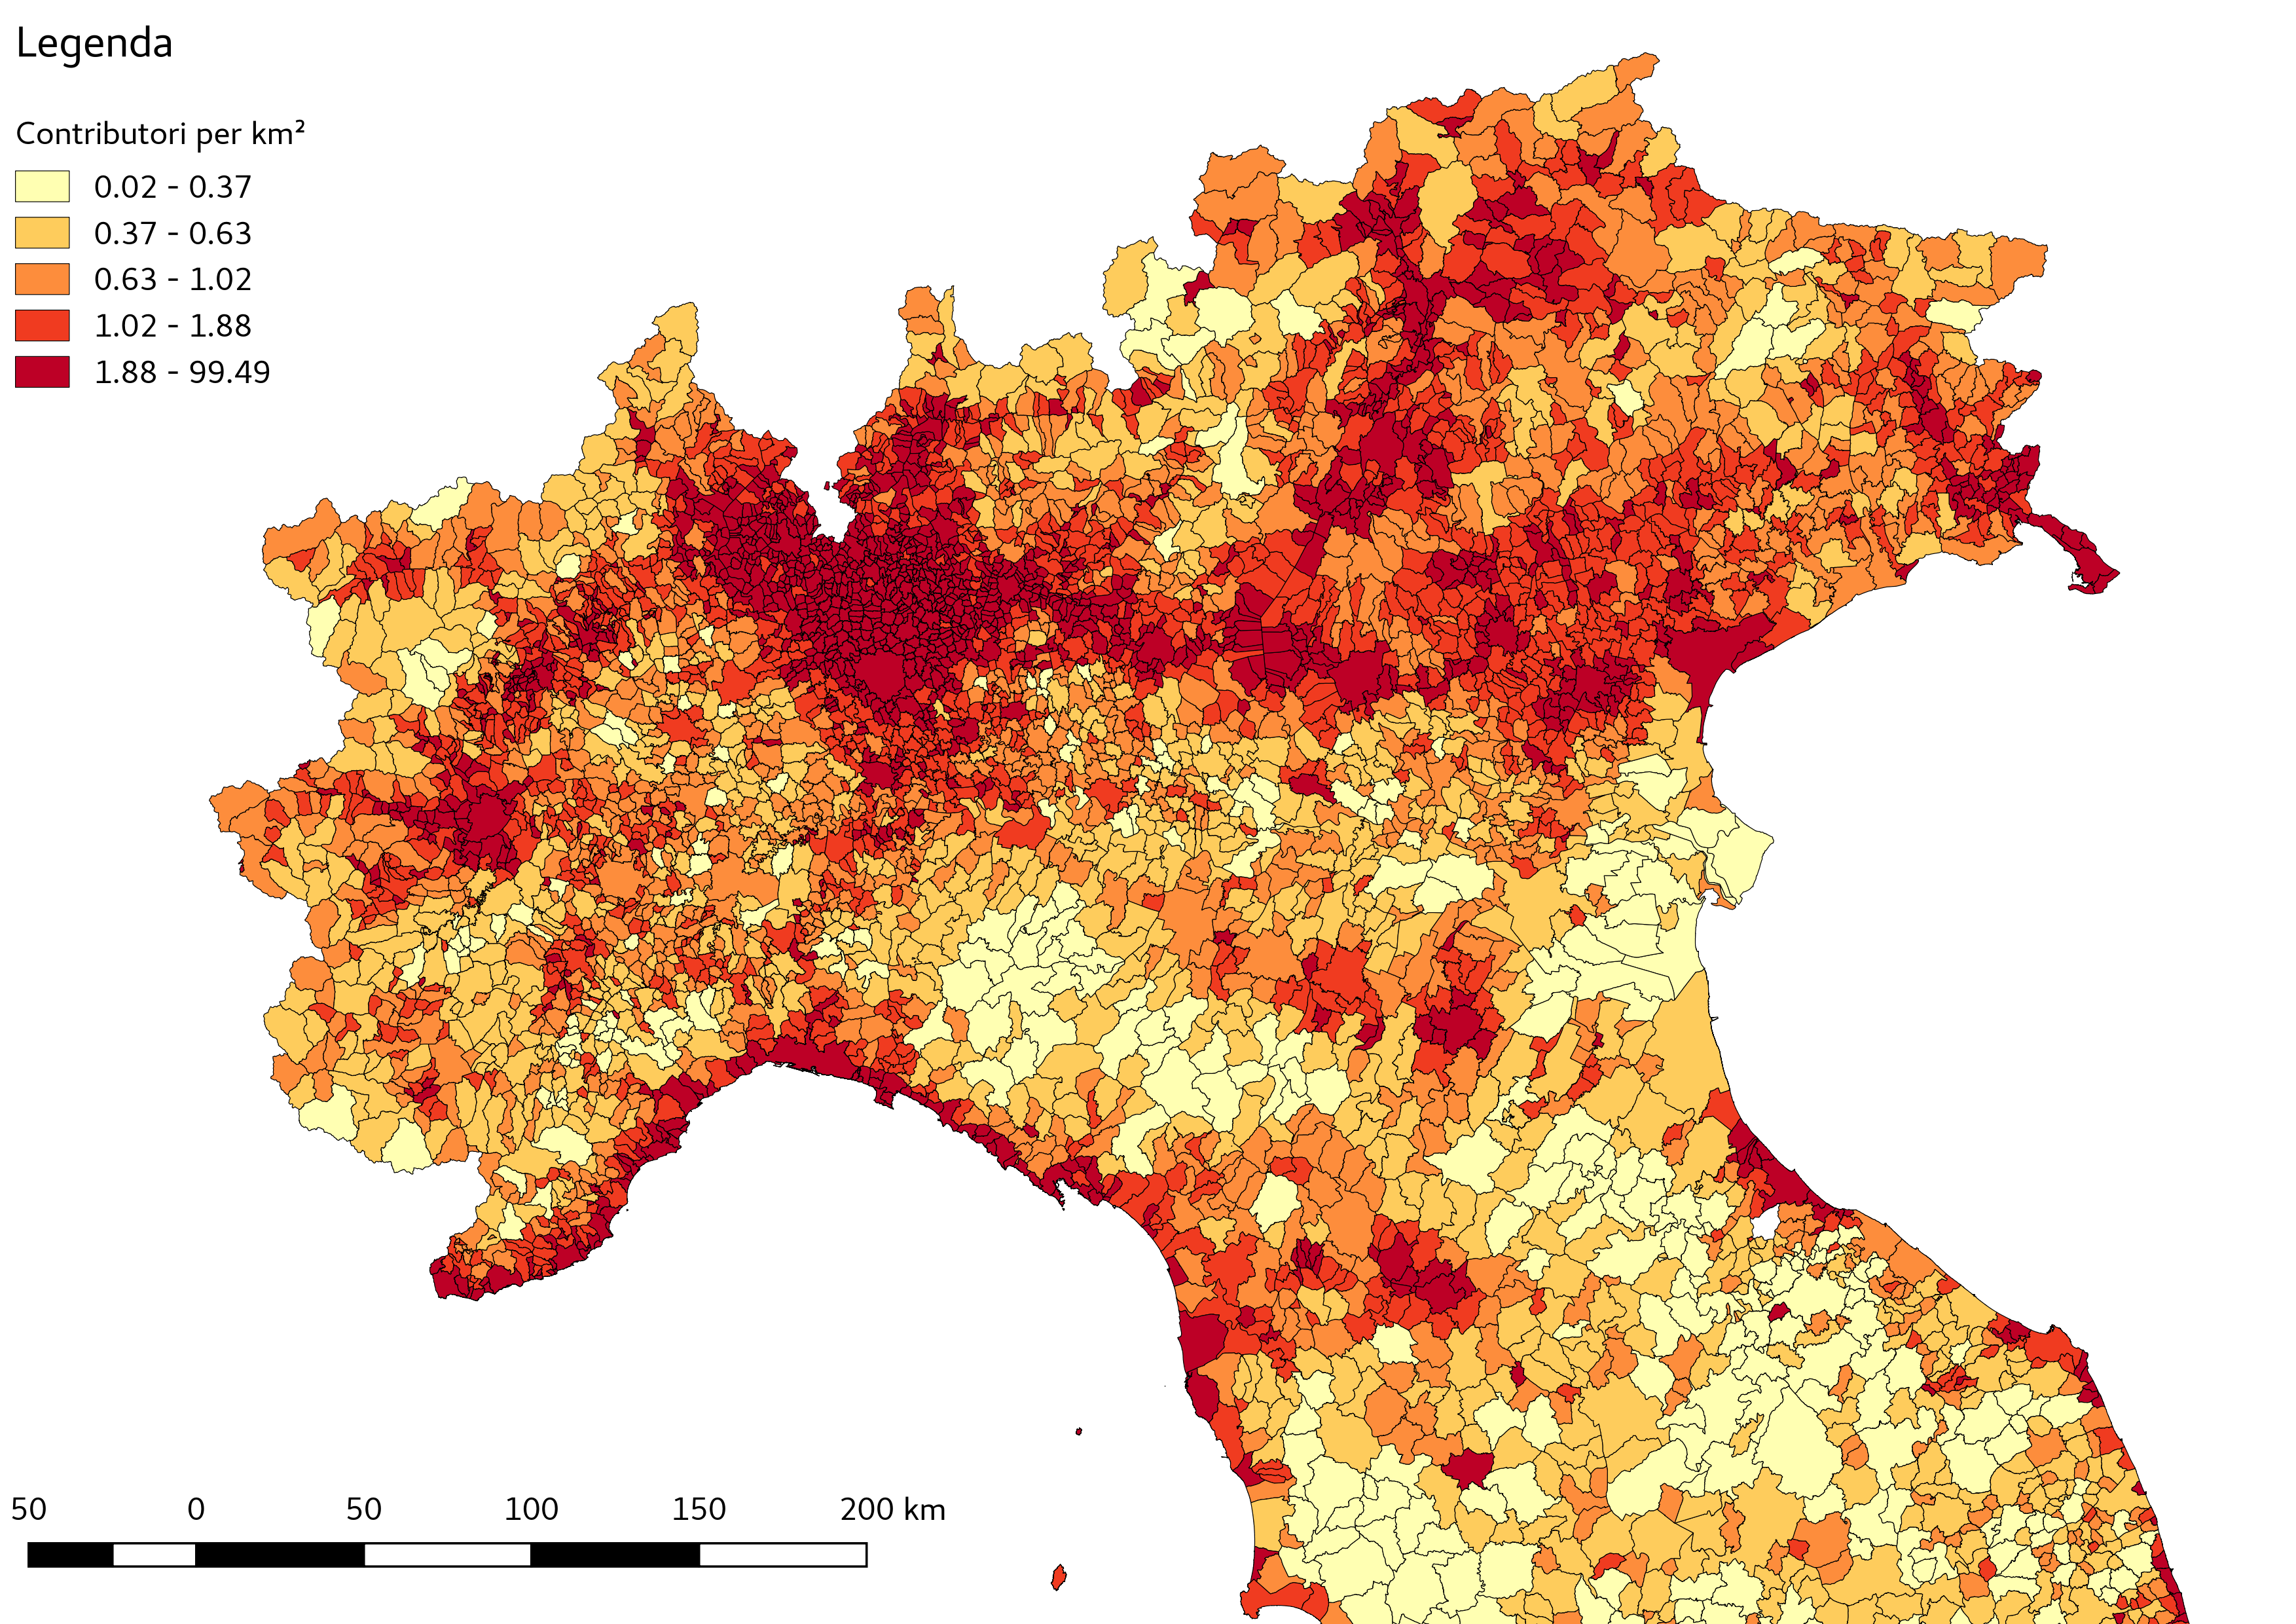
\includegraphics[width=1\textwidth]{Images/contributors_density_north.png}
    \caption{GFOSS day/Merge-IT 2018 – North Italy, contributor density}
    \label{fig:contributors_density_north}
\end{figure}

%\begin{figure}[ht]
%    \centering
%    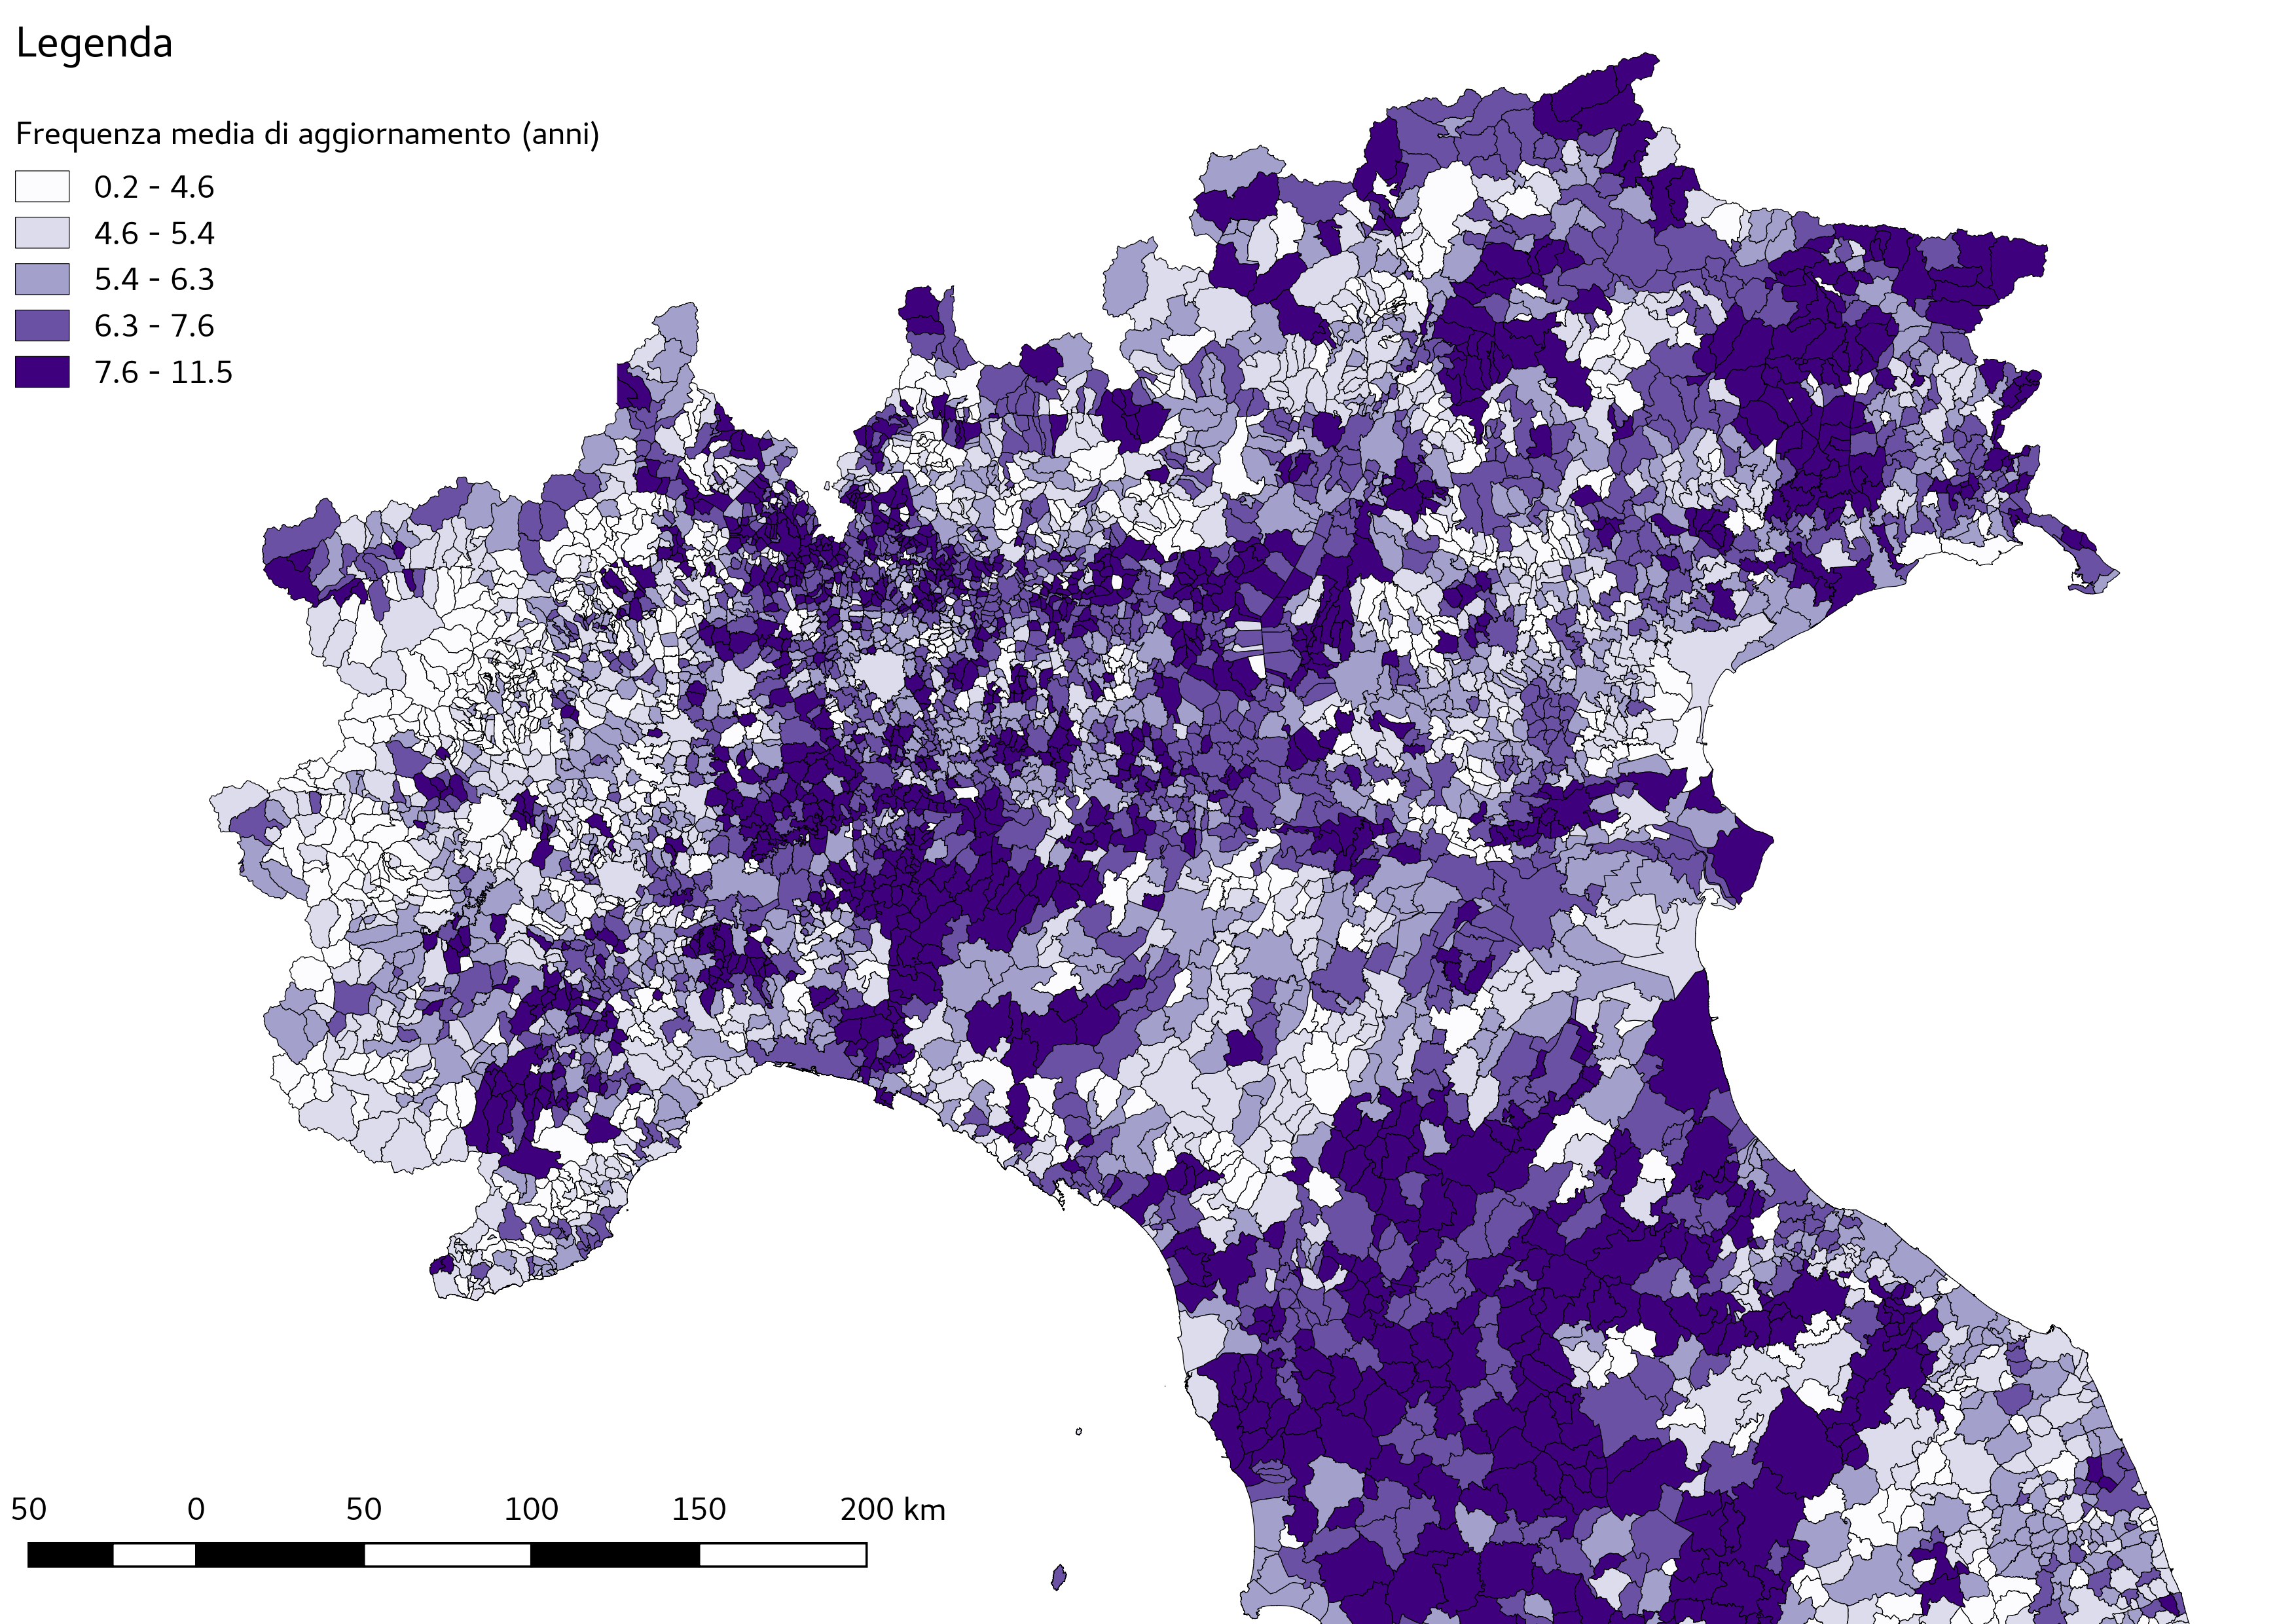
\includegraphics[width=1\textwidth]{Images/rate_avg_north.png}
%    \caption{GFOSS day/Merge-IT 2018 - North Italy, average update frequency}
%    \label{fig:rate_avg_north}
%\end{figure}

\subsubsection{FOSS4G 2018 – Dar es Salaam}

In June 2018, a quality assessment report of the Dar es Salaam area (Tanzania), which has been the venue for the FOSS4G 2018 conference, has been published, with the title: \textit{“An open source approach for the intrinsic assessment of the temporal accuracy, up-to-dateness and lineage of OpenStreetMap”}, by Marco Minghini, prof. Maria Antonia Brovelli and Francesco Frassinelli \cite{minghiniOpenSourceApproach2018}.

Such report shown the evolution of the mapping processes in the area, showing that the vast majority of nodes in the city centre of Dar es Salaam were created in 2015, when the Dar Ramani Huria project was initiated. The mapping activity then gradually continued towards the city outskirts in 2016, 2017 and 2018, the latter clearly showing an increased mapping attention on the northernmost area as well as on more or less isolated areas on the west/south-west side of Dar es Salaam. In particular, the set of cells departing along an almost horizontal line from the city centre to the west side of the city correspond to the location of the towers carrying electricity cables (tag \textit{power=tower}). The average date of last edit of nodes confirms the same trend. In fact, only a small portion of the nodes created before the end of 2015 was later updated, while mapping in 2018 focused almost exclusively on the peripheral areas.

7 different maps with aggregated data have been generated and described, using different criteria, such as node and contributor count, average of creation time, last edit, number of contributors, update frequency and versions.

The report has been cited 6 times, according to Google Scholar.

\begin{figure}[ht]
    \centering
    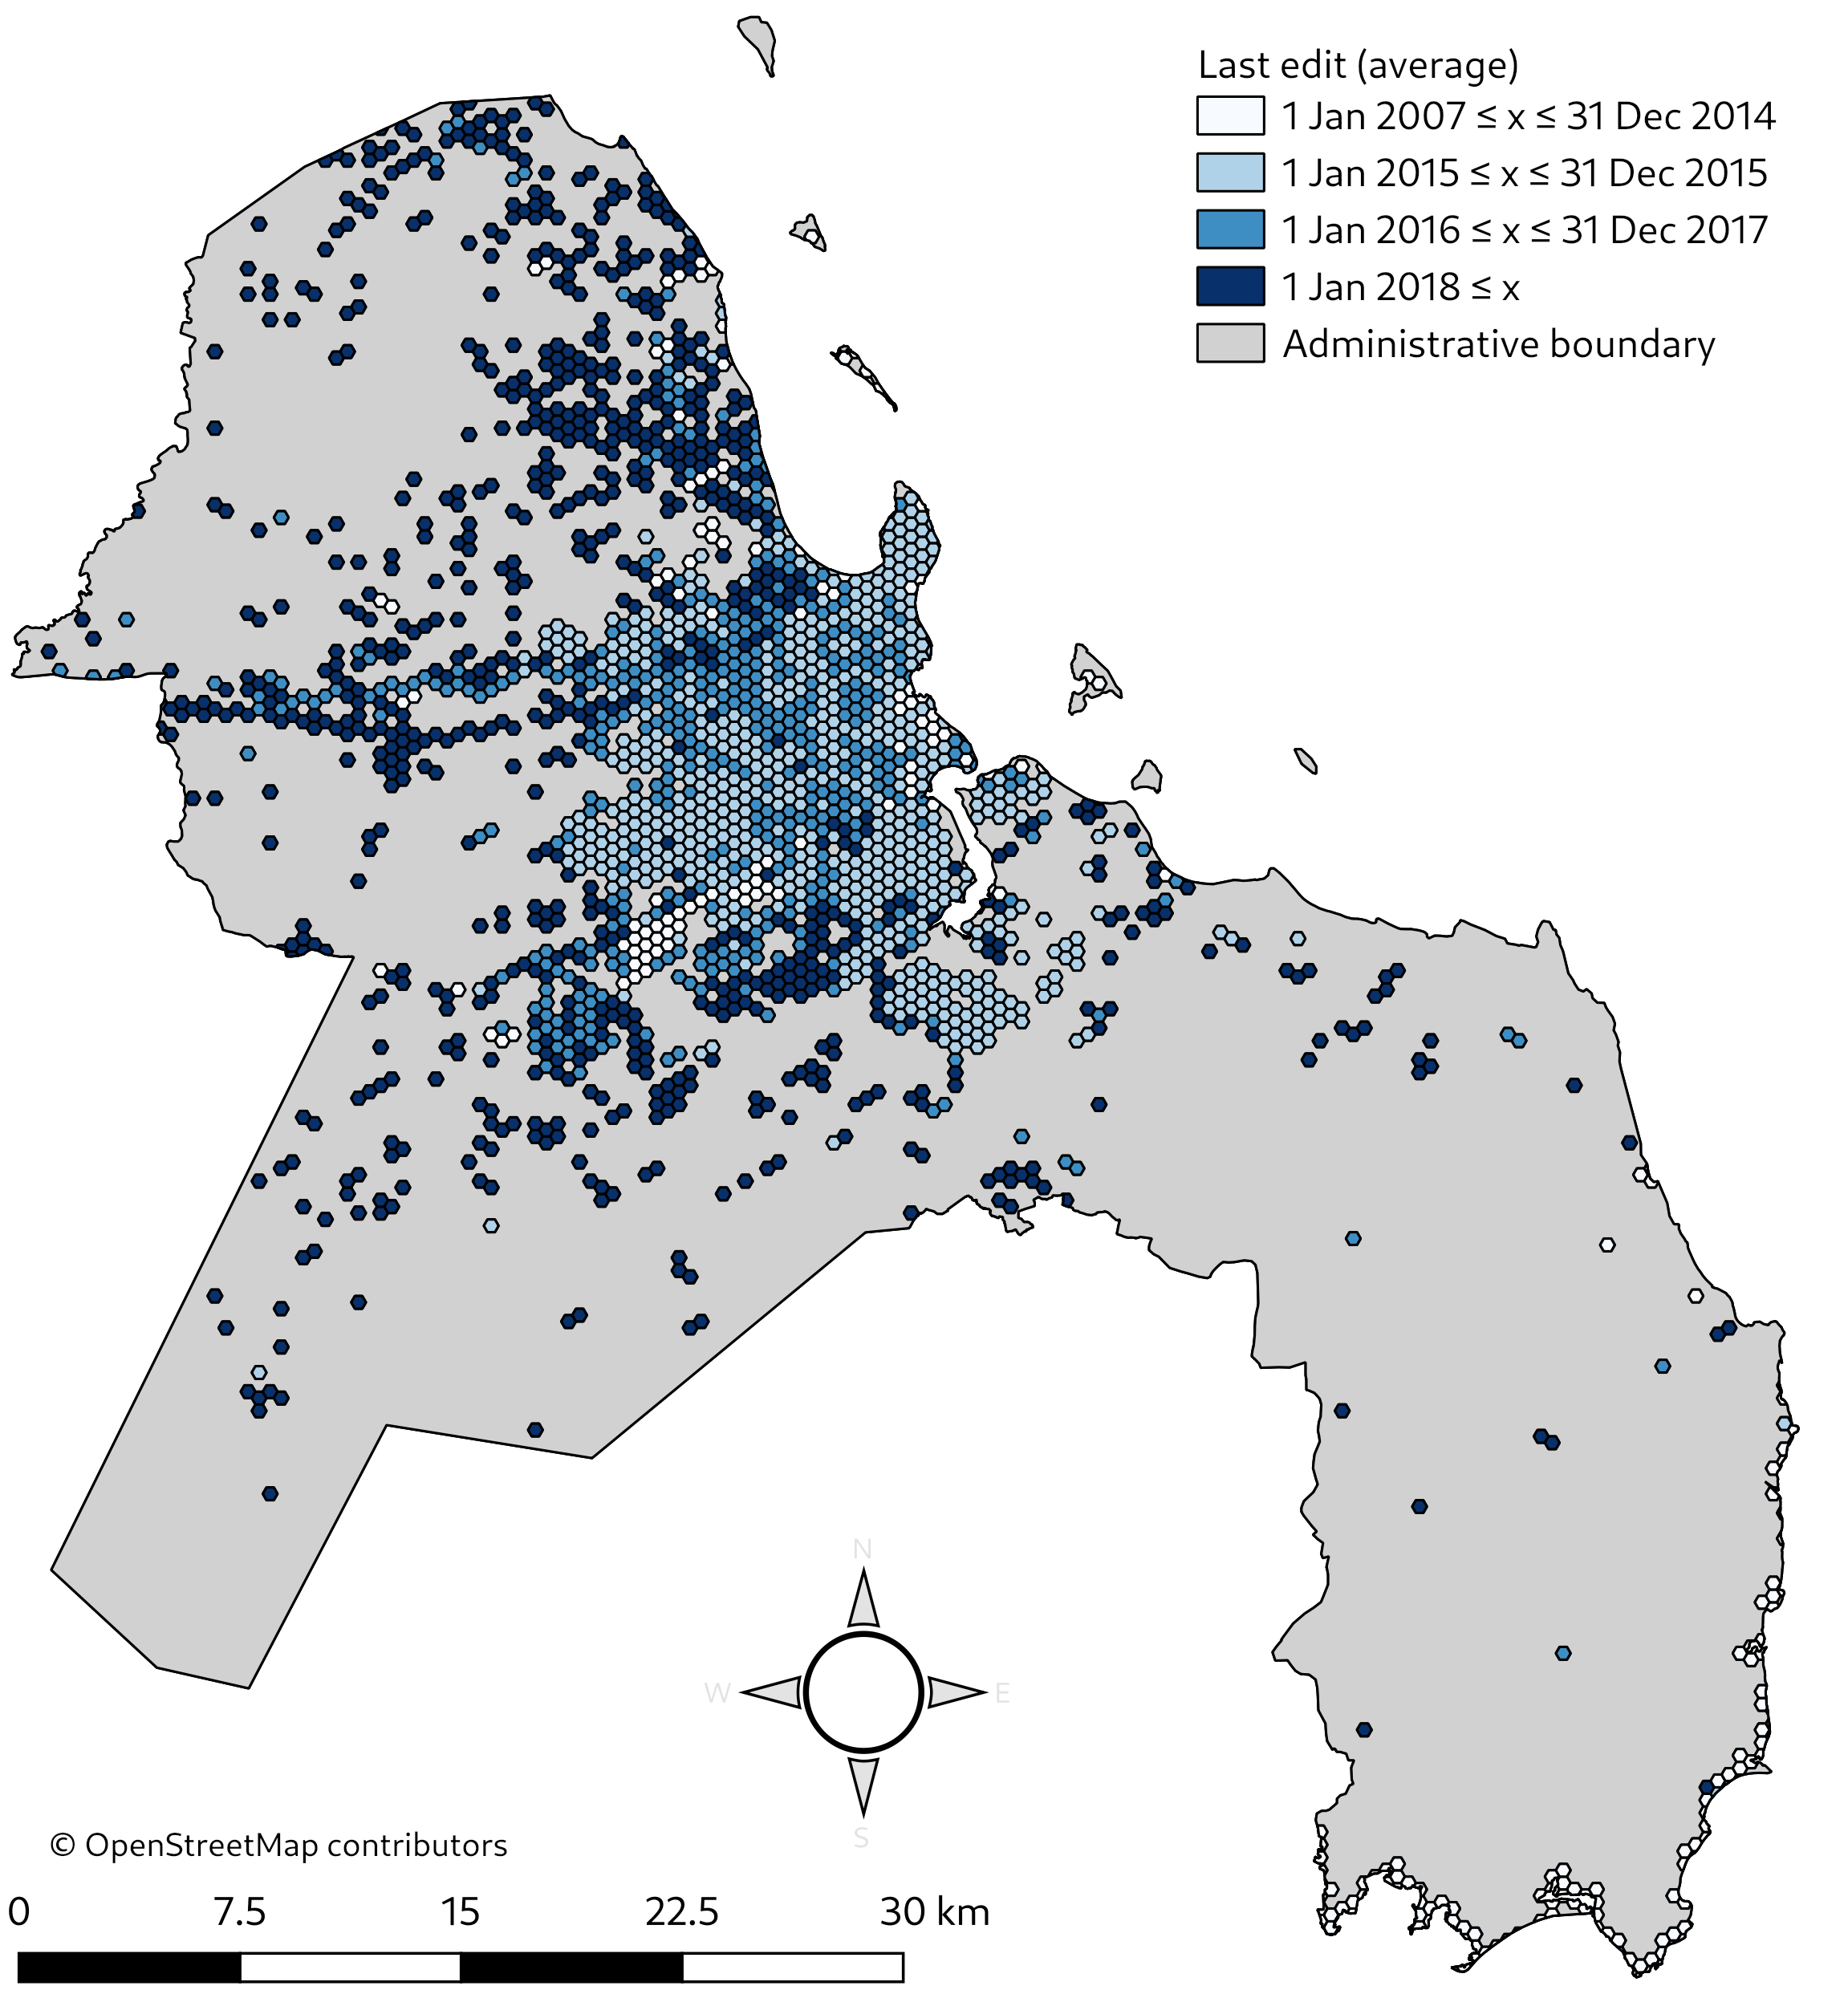
\includegraphics[width=0.8\textwidth]{Images/dar_es_salaam_lastedit.png}
    \caption{FOSS4G 2018 – Dar es Salaam, average last edit}
    \label{fig:dar_es_salaam_lastedit}
\end{figure}

The 31st August 2018, the result of the report has been presented at the FOSS4G conference in Dar es Salaam.

\subsubsection{SOTM 2018 and SOTM 2019}

The software has been adapted to analyse the city of Milan and the results have been shown at the academic track of the State of the Map conference (the annual international conference of the OpenStreetMap community) in Politecnico di Milano, the 29th of July. The presentation title was \textit{“Intrinsic assessment of the temporal accuracy, up-to-dateness, lineage and thematic accuracy of OpenStreetMap”}, presented by Francesco Frassinelli, co-authored by Marco Minghini and prof. Maria Antonia Brovelli \cite{frassinelliIntrinsicAssessmentTemporal2018}.

In such specific context, the personal knowledge of the examined area allowed to suppose various interpretations to the shown results. A strong correlation has been found between the number of revisions and busy roads, as well as high number of contributors in areas where mapping parties happened. It has also been observed that update frequency is mostly homogeneous across the city, with the suburbs being slightly more updated; that could hint that the city centre of Milan is mostly complete from a mapping perspective and new features are created in the suburbs, where there could be more features that still need to be added to the OSM database.

\begin{figure}[ht]
    \centering
    \includegraphics[width=0.9\textwidth]{Images/creation_average.png}
    \caption{SOTM 2018 – Milan, average creation time}
    \label{fig:creation_average}
\end{figure}

The data have then been further used to find spatial correlation patterns using QGIS Hotspot Analysis plugin; the results have been presented at the academic track of SOTM 2019 in Heidelberg, Germany, with a report named \textit{“Intrinsic assessment of OpenStreetMap contribution patterns through Exploratory Spatial Data Analysis”}, by Marco Minghini, Daniele Oxoli, Francesco Frassinelli and prof. Maria Antonia Brovelli \cite{minghiniIntrinsicAssessmentOpenStreetMap2019}.

\subsubsection{Peer-reviewed paper (September 2019)}

A peer-reviewed software paper titled \textit{“OpenStreetMap history for intrinsic quality assessment: Is OSM up-to-date?”}, by Marco Minghini and Francesco Frassinelli, has been published in “Open Geospatial Data, Software and Standards” \cite{minghiniOpenStreetMapHistoryIntrinsic2019}.

The paper reviewed the existing software for handling, showing and analysing OpenStreetMap history, comparing them to the \textit{Is OSM up-to-date?} application, and it has been cited 35 times, according to Google Scholar.

\section{Running aggregated analysis in real-time}

The final goal for this research was to make the web application converge with the methods used for aggregated analysis. This has proved to be a major technical challenge, as the needs of a web application (which is assumed to show results with little delay) and the ones of spatial analysis over larger areas (thus requiring way more data to fetch and handle) are in conflict.
Exploring different solutions and approaches, running benchmarks with different parameters and experimenting with different techniques allowed to move towards such result.

An important simplification can be splitting the globe into a grid, which is needed in case of pre-computed statistics, but can also make caching easier. A hexagonal grid would better represent reality, but is more complex to handle compared to a square grid, since APIs commonly used require a rectangular bounding box, and spatial operation usually simpler when using a square grid. 

\subsection{Evaluated options}

\subsubsection{Pre-computed statistics}

The idea behind pre-computed statistics is to have a long-running task which is executed regularly (like once every week or month), which stores just the result of the analysis for each cell or tile of the globe. Such approach is based on the following assumptions:

\begin{itemize}
\item the criteria and methods used satisfy the most common and interesting user needs, as the original non-aggregated data is discarded and additional statistics cannot be computed; for example, if no standard deviation has been computed in advance, there is no way to compute it afterwards, except by implementing a software change and run the computation again;
\item aggregation of aggregated data can be performed: it should be possible to group statistics together, to produce data to be displayed at lower scales; for example, aggregating two bounding boxes represented by the averaged revision number can be done if the information about the number of features within the two bounding boxes is stored; otherwise the total average cannot be computed.
\end{itemize}

By relying on square web tiles \cite{TiledWebMap2022}, it can be easily computed that the number of tiles that should be computed at a zoom level 18 (scale $ \approx 1 : 20 000 $\footnote{The scale of an individual varies when using different screens, resolutions or when the tile renders data at high latitudes, since the \textit{Web Mercator projection}, commonly identified as EPSG:3857, is a variant of the Mercator projection}) is large $ 4^{18} = 68 719 476 736 $ \cite{ZoomLevelsOpenStreetMap}. If we assume that the Earth surface 71\% covered by water and nodes with attributes on water are very rare, the number of tiles would drop to $ 4^{18} \times (1-71/100) \approx 20 000 000 000 $. The storage space needed to store 5 16-bit precision float numbers (4 bytes each) for all the terrestrial tiles would then be $ 20 000 000 000 \times 5 \times \SI{4}{bytes} \approx\SI{400}{GB} $ at least. This does not seem very efficient, since the whole OSM history is $ \approx\SI{100}{GB} $: four times smaller than such a hypothetical file containing pre-computed statistics. Such difference could be explained by the fact that wide areas of land in OSM have no data; it could be that the final result would be much smaller, if the data store in the resulting file are tightly packed.
Handling a regular update, conversion and indexing using a custom format could still require an important amount of computational resources when working on such a big dataset.

\subsubsection{Database conversion}

Storing the data in a Postgres/PostGIS database could be an alternative, but storage requirements are over 1 TB and the conversion require some days using osm2pgsql \cite{Osm2pgsqlBenchmarksOpenStreetMap}.
There are alternative methods to import data, such as using a Postgres Foreign Data Wrapper (FDW) for reading OSM PBF \cite{pikulikOSMPBFForeign2022}, but storage requirements are assumed to be similar. 
Conversion of PBF files to a database is also made by OSHDB \cite{raiferOSHDBOpenStreetMapHistory2021}, which powers Ohsome.
Avoiding conversion of planet files (PBF or BZIP2-compressed XML) in the first place would greatly help, but as they do not have a spatial index, this should be generated first. As there is no ready available solution for that and the development of such system would require an additional effort, such solution has then been discarded.

\subsubsection{Cloud services}

AWS Athena \cite{AmazonAthenaServerless} is a service provided by Amazon. It has been evaluated to see if it could have been a viable solution. Amazon also has a copy of the OSM planet history file, which can be used for queries. Running joins is not efficient (probably due to not having indexes), and running complex queries require splitting the database into multiple pieces, which seems impractical for the given purpose, so it has been discarded.

\subsubsection{Fetching data from external public API}

Benchmarks between the different methods to retrieve historical data on a larger scale from publicly available APIs have been performed. The area considered is centred across “Città Studi” in Milan and is $ \SI{1}{KM^2} $ wide.
Over such area, Overpass with batched queries needs 3 minutes, OSM API + HTTP 1.1 pipelining 30 seconds, while Ohsome API just 5 seconds. Ohsome would be much slower in case the tags of the previous versions are requested or ways and relations are fetched too, but as the focus of the current research does not focus on these aspects, Ohsome seemed the most promising solution. Ohsome API can also return a GeoJSON object, which could be fetched directly from the browser, but the computation would require more time, as the load would be put on the client instead of an intermediate server. The result could not be cached and shared across multiple clients.

Techniques such as caching, parsing and processing while fetching, and data compression can be hugely beneficial, as the data should be retrieved over the network.

\subsection{Chosen option}

Ohsome has been then chosen as data source for aggregated analysis from version 1.6, combined with a caching mechanism from version 2.0, to further improve performances and reduce the load on the Ohsome API server.

\subsubsection{Displaying data efficiently}

The software initially displayed all the nodes as different features on a map. This approach does not work when hundreds of nodes are displayed on the screen, for two reasons: nodes overlapping and client performances (both bandwidth and rendering). 

The problem has been initially addressed in version 1.8, by using a popular extension for Leaflet, called \textit{Leaflet.markercluster} \cite{LeafletMarkercluster2022}, which shows a single circle for each group of close nodes. The colour of such circle varies from green, to yellow and orange, based on the number of nodes in the group. This is useful for a heatmap-like visualization, but it clashes against how colours are used in the web app, as colours represent a quality indicator. Altering how the colour is assigned to group, it is possible to use the same criteria.

Using Leaflet.markercluster is acceptable until thousands of nodes are shown on the screen. It has been tested the possibility of generating PNG images, each representing a group of nodes, and serve them as tiles, following the common Tiled Web Map convention \cite{TiledWebMap2022}. Such a test ended successfully, so the approach has been adopted to aggregate data on a larger scale.

\subsubsection{Serving data efficiently}

The software moved away from using Hug \cite{HugapiHug2022}, due to the inability to stream data, and adopted uwsgi \cite{unbitUnbitUwsgi2022} with Flask \cite{Flask2022}. That allowed serving static files independently of the Python version and run multiple Python processes and threads.

During the development of version 2.0, which added support for tiles, this approach shown some limitations, as each tile is generated from a different HTTP request, so dozens of concurrent requests are produced by a single client. Since it is not possible to have many threads without incurring in performance penalties due to the Python global interpreter lock and memory usage scales linearly with the number of processes spawned, the software stack for the server had to change again.

Version 2.0 and above use aiohttp \cite{AsyncHttpClient2022} combined with gunicorn \cite{GunicornPythonWSGI}, which allowed to fetch and serve many tiles concurrently with a lower latency and resources.

\chapter{Final solution}
\label{ch:final_solution}%

The main result of this research has been the development of the \textit{Is OSM up-to-date?} \cite{OSMUptodate,frassinelliOSMUptodate2022}, as well as its deployment as a publicly available service over the web for free, maintained, updated and developed for almost 5 years.

\section{Usage}

The software consists can be used with its web interface or by connecting a GIS software to it. In the latter scenario, an external software can further analyse and process the GeoJSON produced by fetching the historical data over a defined bounding box using the available API, or by relying on the ability of the software to produce raster tiles.

\subsection{Web interface}

The web interface is made by a map and a bar. Data is automatically loaded when the user lands on the page for the first time, and it is updated when the boundaries or the settings changes.

\begin{figure}[ht]
    \centering
    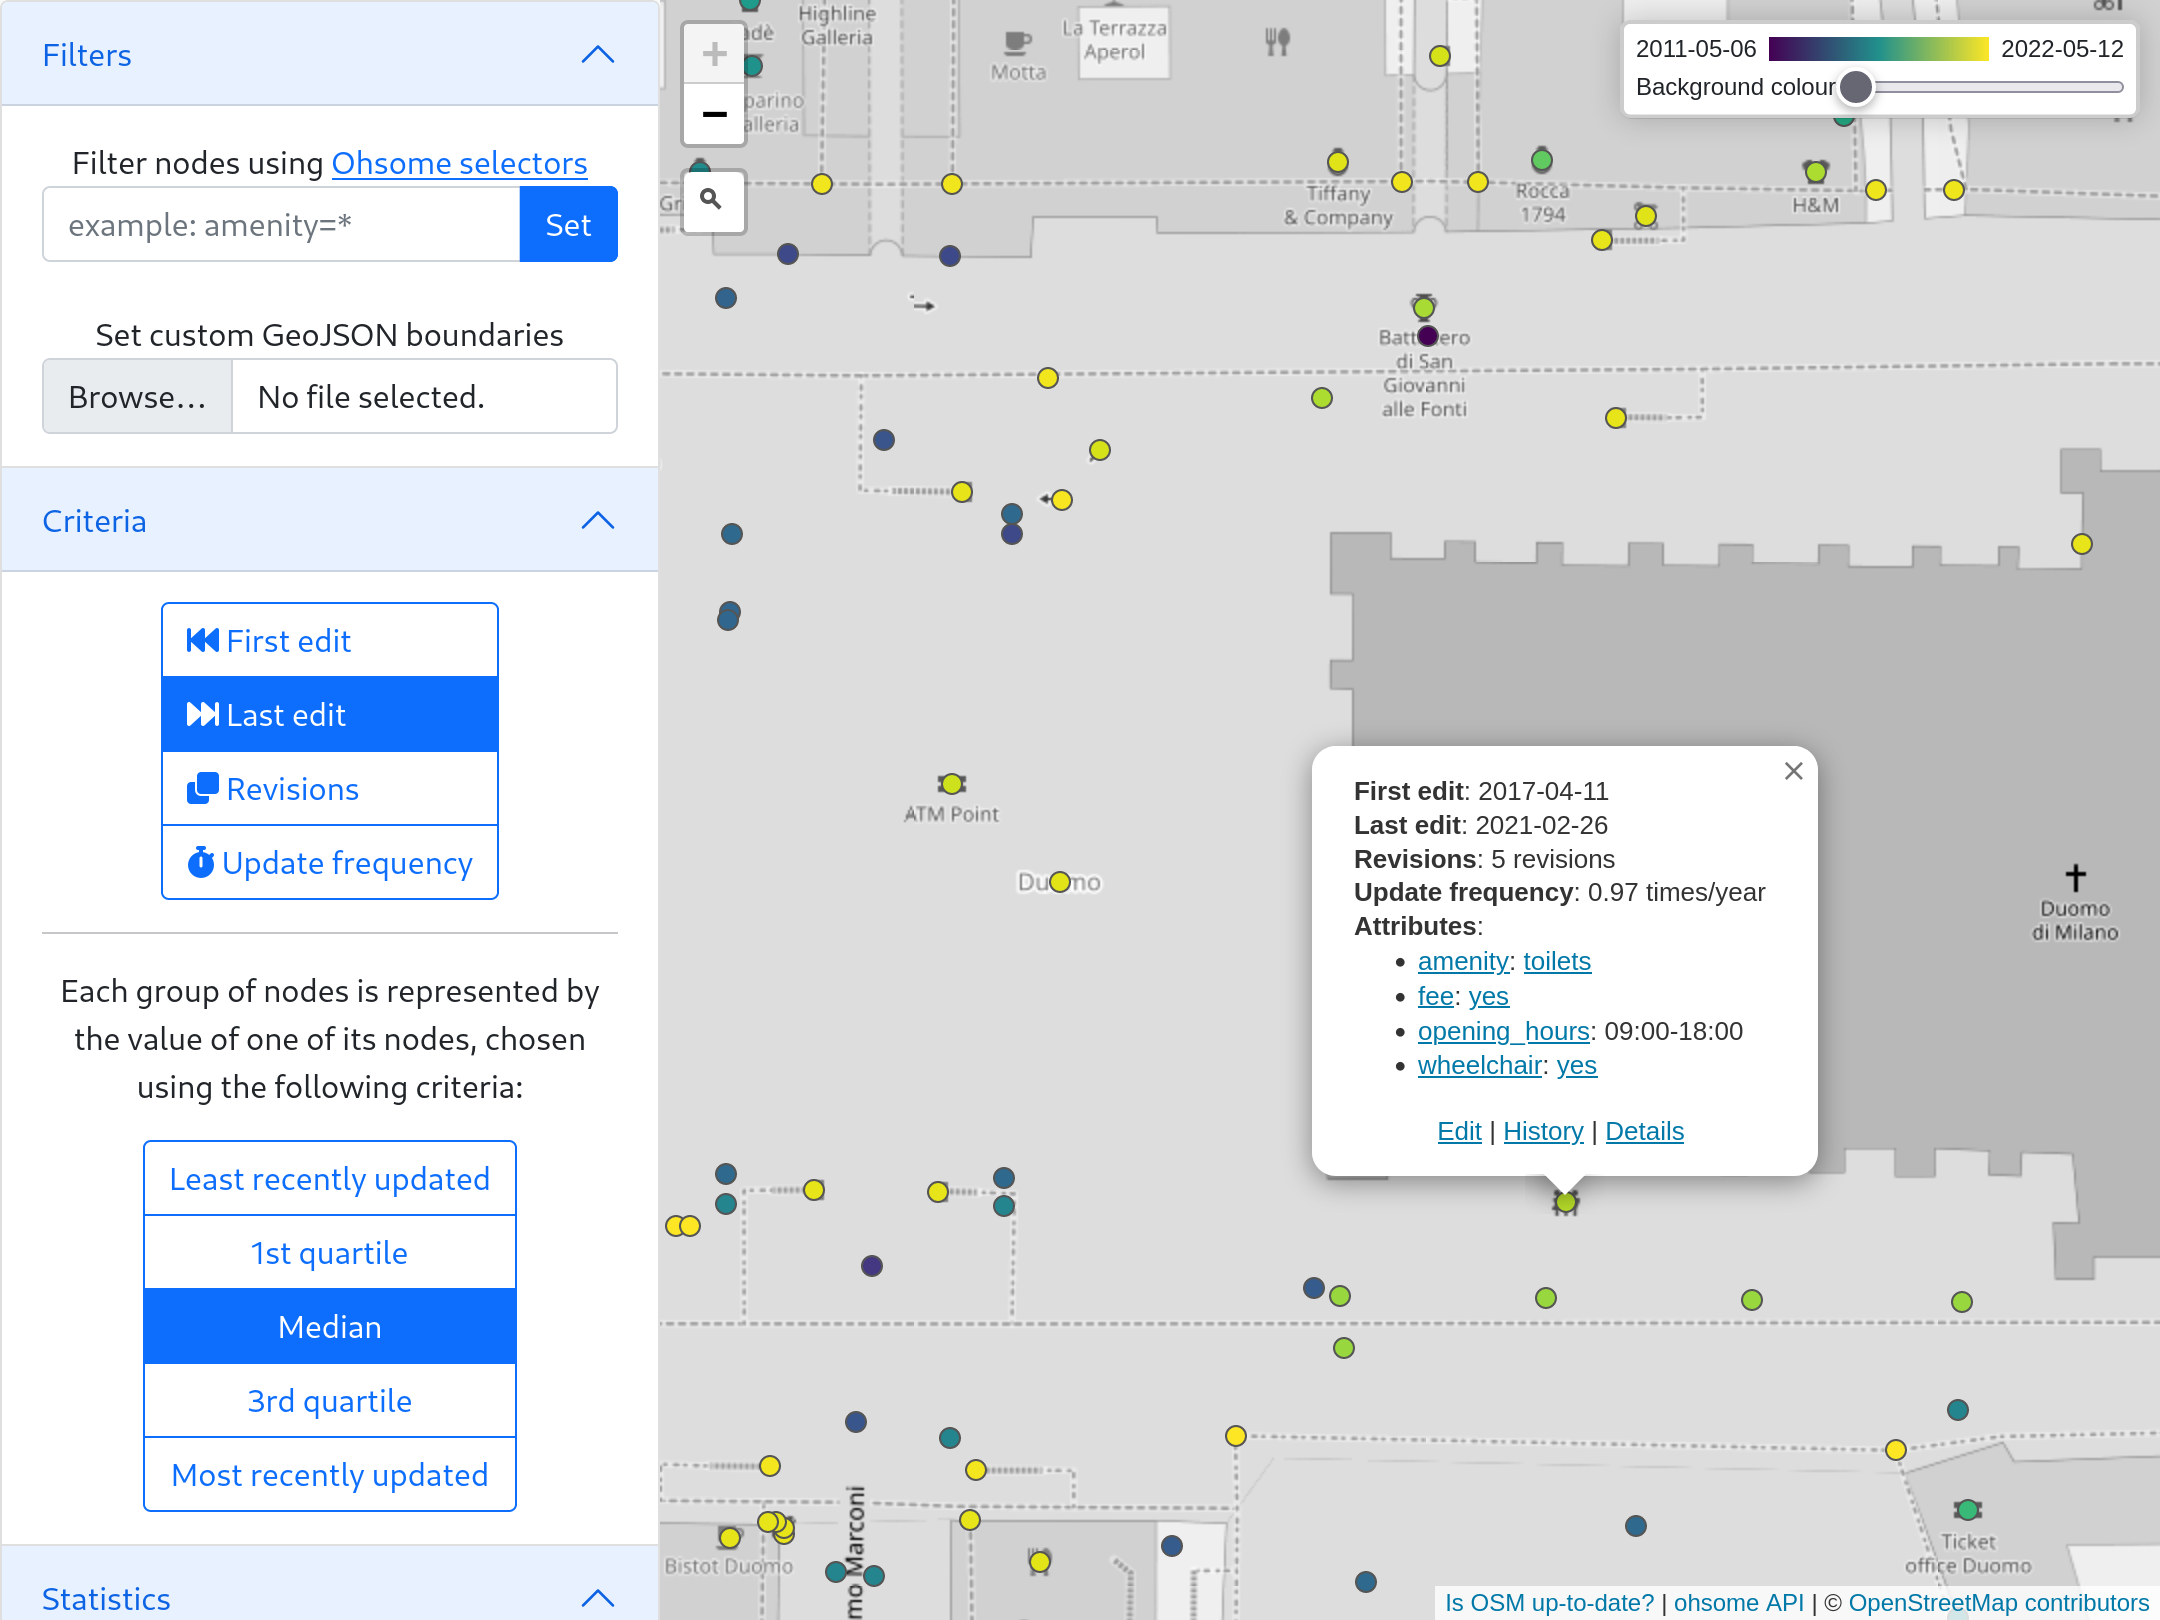
\includegraphics[width=1\textwidth]{Images/level19_popup.png}
    \caption{Web app – Zoom level 19, individual nodes with pop-up}
    \label{fig:level19_popup}
\end{figure}

\subsubsection{Map}

The map shows the current area of interest, and it is made by:
\begin{itemize}
    \item the standard OpenStreetMap \textbf{base map};
    \item the \textbf{nodes} (if any), rendered individually as coloured circles at zoom level 19 (figure \ref{fig:level19_popup}), or as group between level 17 and 18 (figure \ref{fig:level17}), or as tile between level 12 and 16 (figure \ref{fig:level16});
    \item the \textbf{legend}, placed in the top-right corner, constituted by:
    \begin{itemize}
        \item a \textbf{colour bar} representing the colour range, with the minimum and maximum values placed at its extremes;
        \item a \textbf{slider} to convert the base map to greyscale, which is meant to increase the contrast between the nodes and the background; the position of the slider defines the proportion of the conversion, which goes from full greyscale (default setting) to full colour;
    \end{itemize}
    \item \textbf{zoom controls}, placed in the top-left corner;
    \item \textbf{search button}, placed below the zoom controls, which opens a search bar with autocompletion when pressed/clicked;
    \item an animated \textbf{loading spinner}, which appears when the map is updating;
    \item \textbf{attribution}, mentioning OpenStreetMap contributors, the Ohsome project and \textit{Is OSM up-to-date?}, linked to its GitHub repository.
\end{itemize}

Clicking or tapping on a node opens a pop-up, shows the computed values of the node (first edit, last edit, revisions, update frequency) as well as the node attributes (fetched asynchronously from OpenStreetMap API). Links to the OpenStreetMap wiki portal are automatically generated for all the keys and values; a regex is used to avoid creating links to uncommon values that are not expected to have their page in the wiki.

The pop-up also has links to the web OpenStreetMap website, to make changes using the editor, get the full history of the node, or get more details.

\begin{figure}[ht]
    \centering
    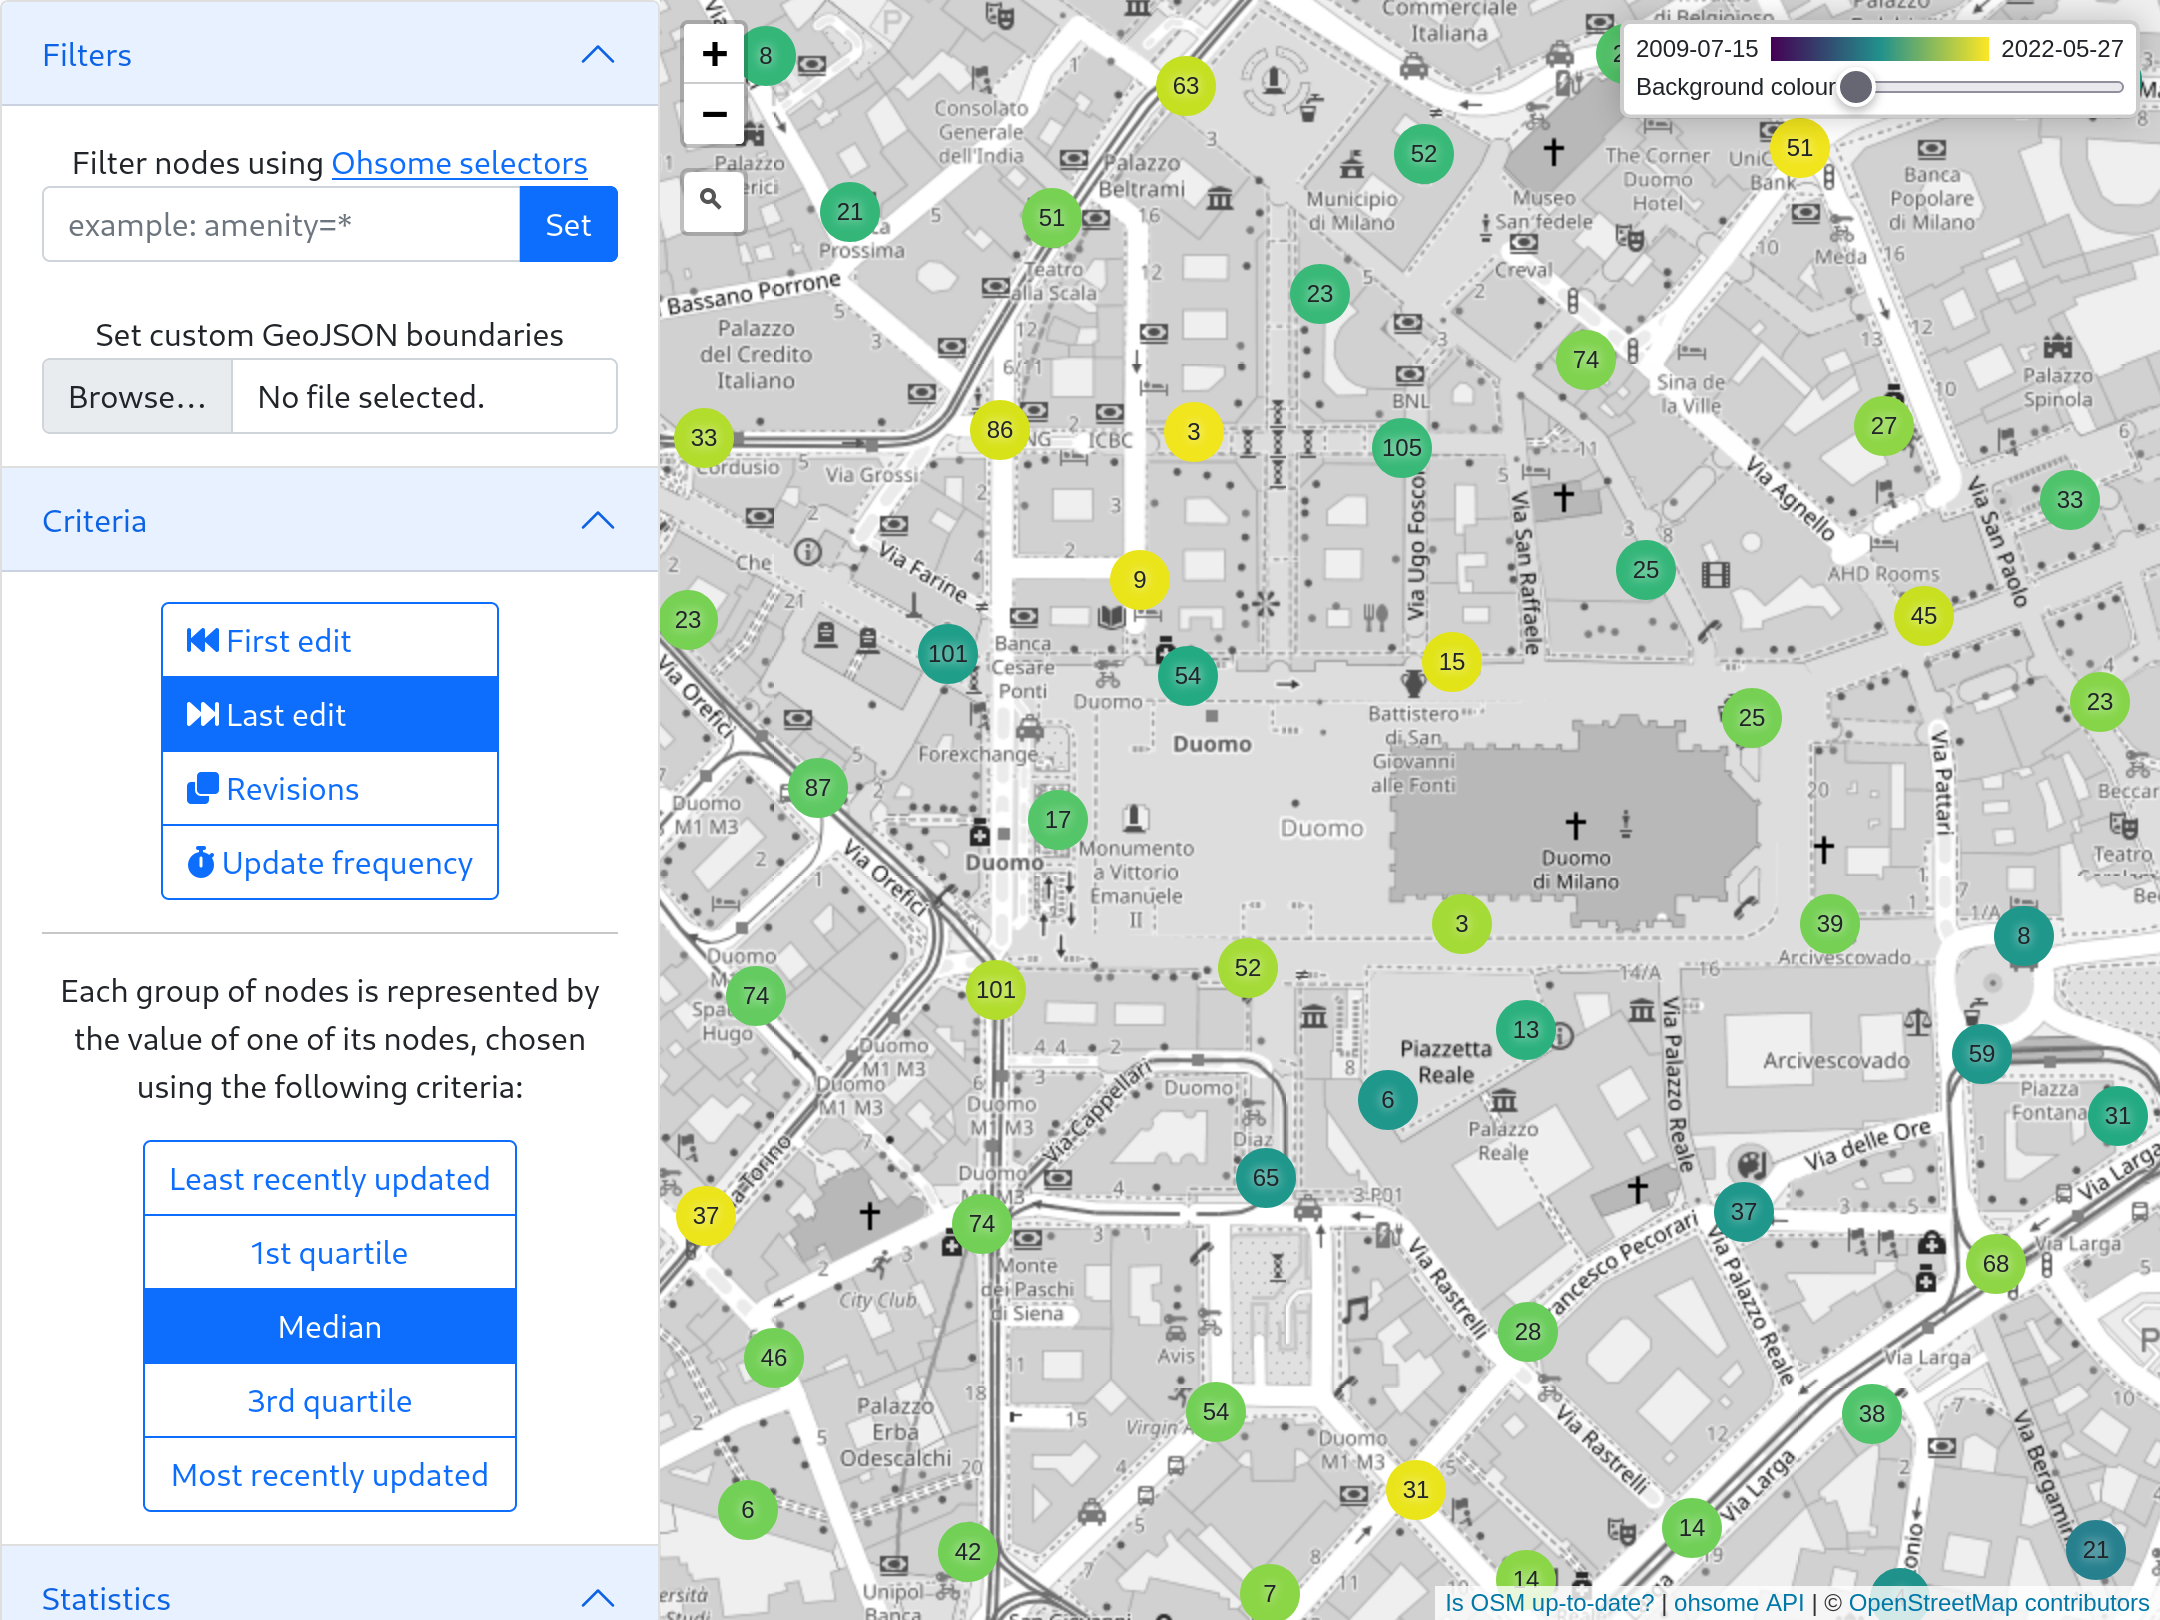
\includegraphics[width=1\textwidth]{Images/level17.png}
    \caption{Web app – Zoom level 17, clustered nodes}
    \label{fig:level17}
\end{figure}

\begin{figure}[ht]
    \centering
    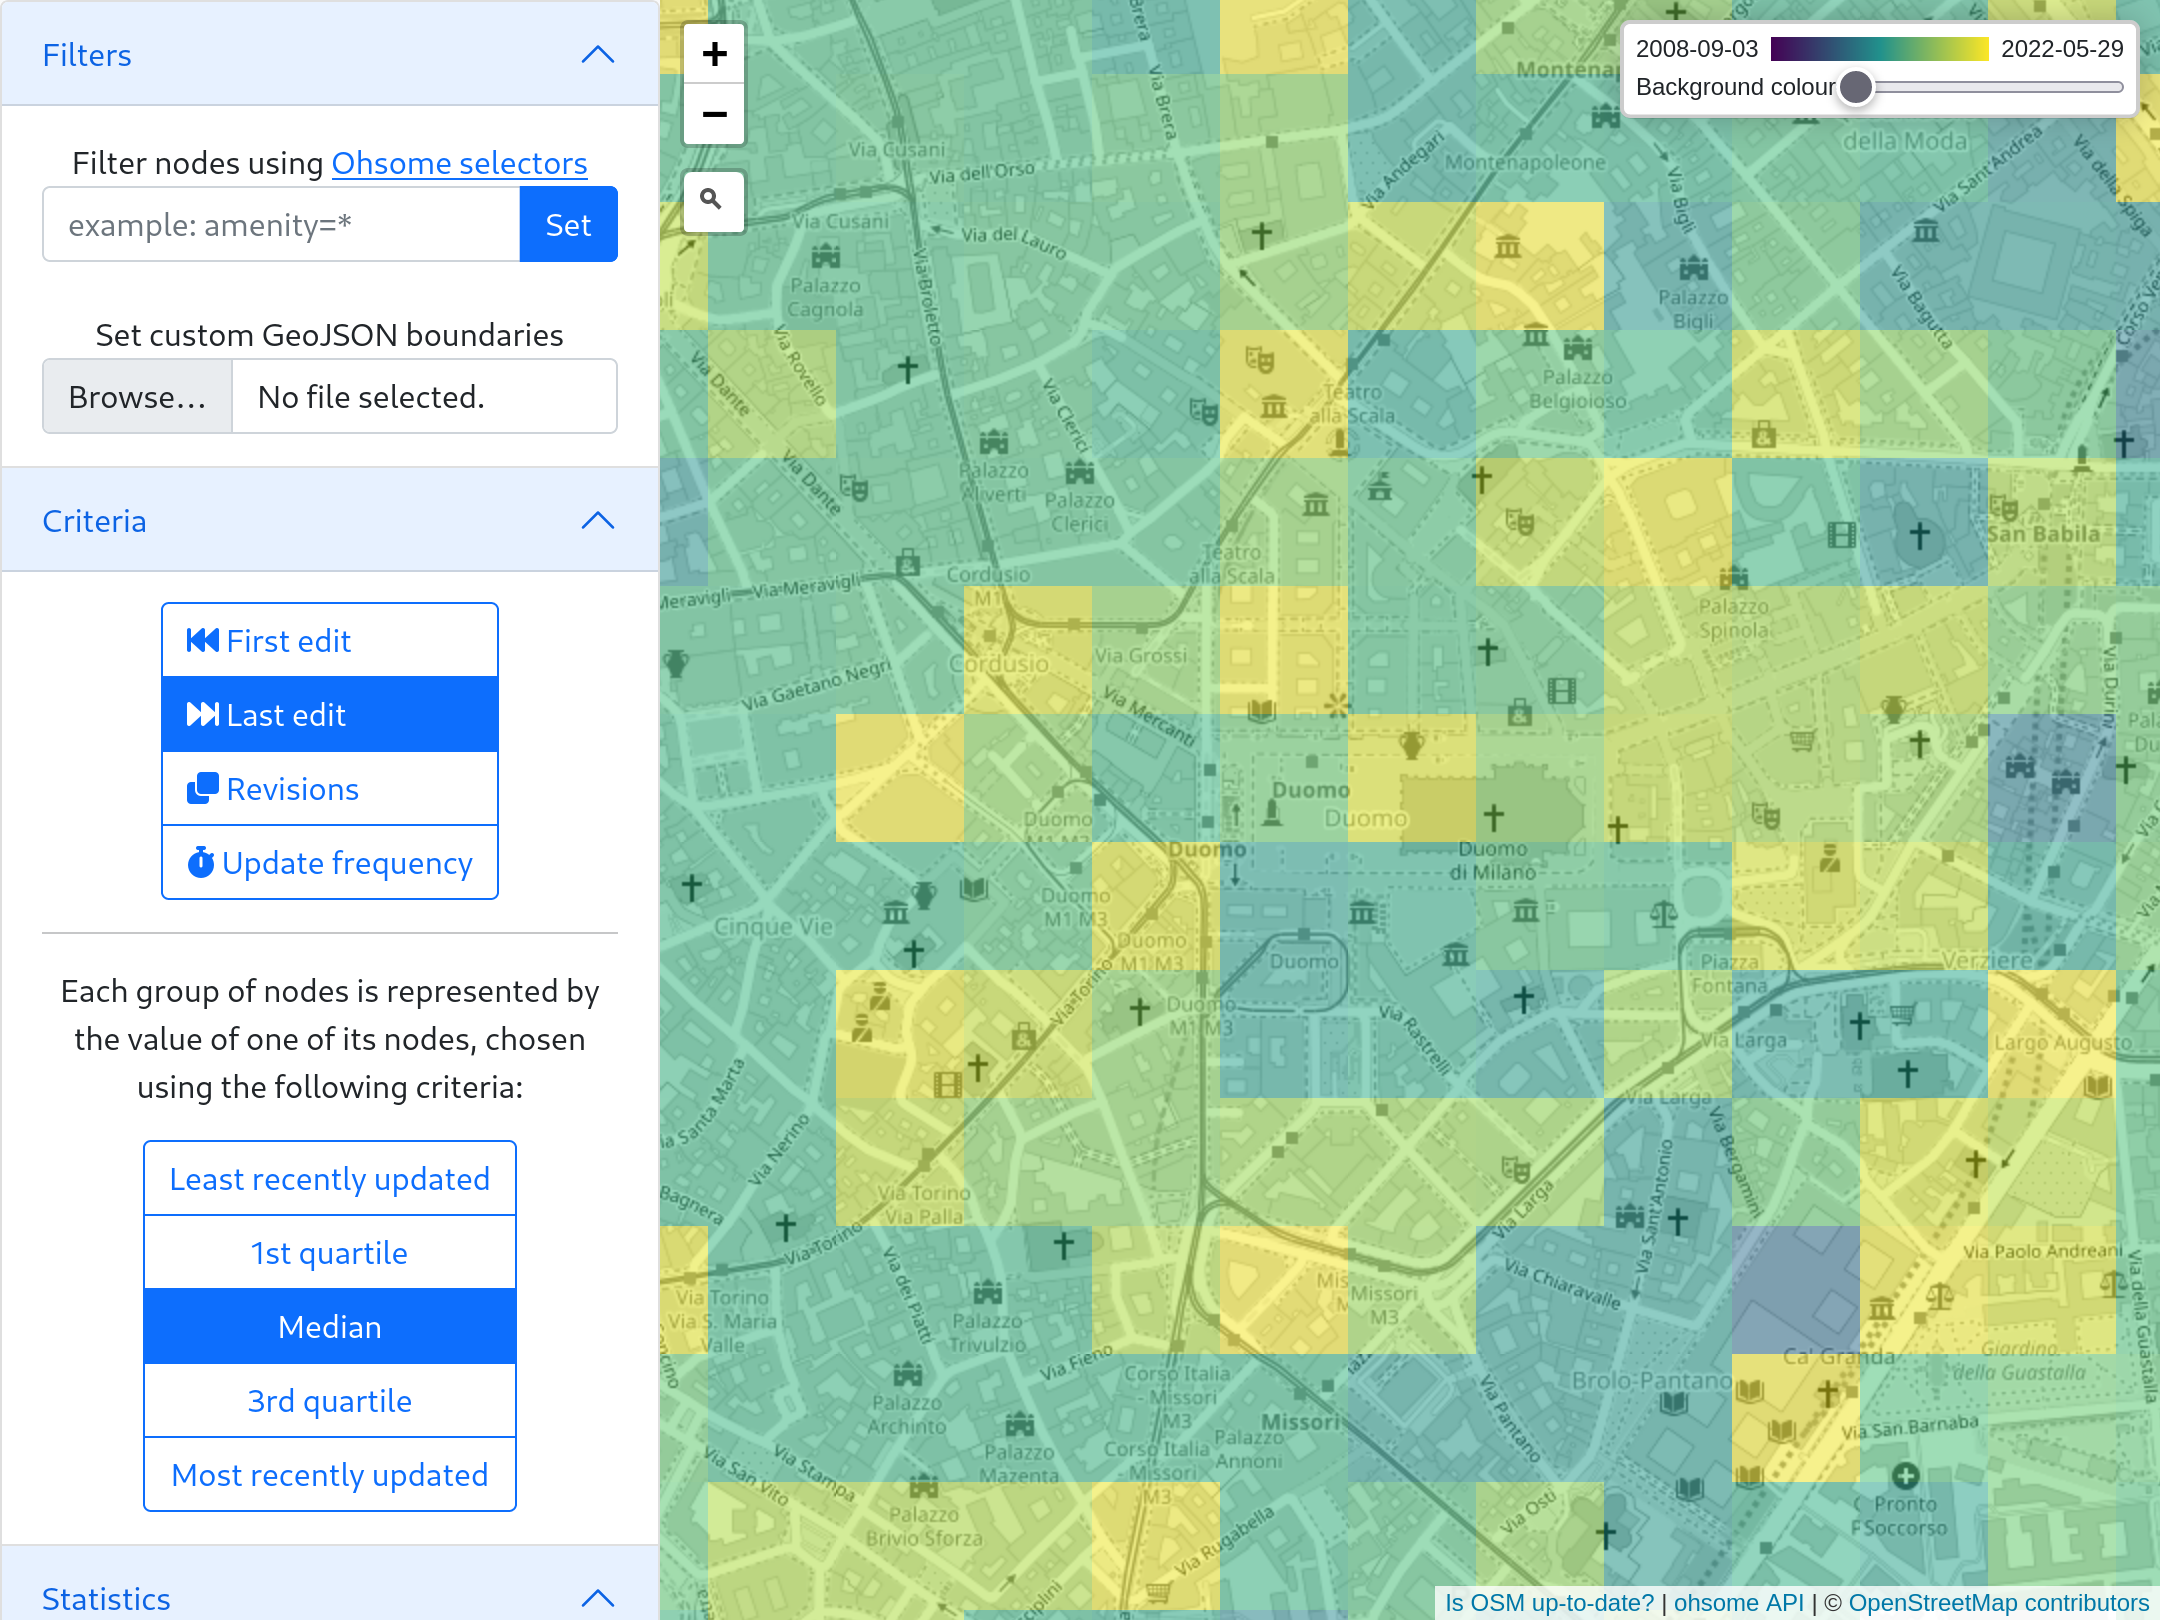
\includegraphics[width=1\textwidth]{Images/level16.png}
    \caption{Web app – Zoom level 16, tiles}
    \label{fig:level16}
\end{figure}

\subsubsection{Left bar}

The left bar is composed by different section that can collapse (expanded by default). These are:

\begin{itemize}
    \item \textbf{Filters}, used to reduce the number of nodes considered, using two mechanisms:
    \begin{itemize}
        \item tag filters, that rely on Ohsome selectors, allowing the user to select only certain keys or values using different criteria;
        \item GeoJSON boundaries, specified with a file input field, which allow the user uploading a set of geometries delimiting the area to be analysed (figure \ref{fig:level12_milano_geojson_shops});
    \end{itemize}
    \item \textbf{Criteria}, split in two sections:
    \begin{itemize}
        \item \textbf{gparameter} to be evaluated, as previously described (see \ref{subsec:criteria_historical}), with the exclusion of the user count (due to Ohsome limitations);
        \item \textbf{grouping criteria}, based on quartiles, which provides five choices:
        \begin{itemize}
            \item minimum value, which is labelled differently based on the criteria that has been selected, so the minimum value button contains the text \textit{Least recently updated} when \textit{Last edit} is chosen as criteria;
            \item 1st quartile;
            \item median (default choice);
            \item 3rd quartile;
            \item maximum value, which is labelled using the same mechanism used for the minimum value, so the minimum value button contains the text \textit{Most recently updated} when \textit{Last edit} is chosen as criteria;
        \end{itemize}
    \end{itemize}
    \item \textbf{Statistics}, which list the values of the quartiles used by the grouping criteria, with the addition of the node count;
    \item \textbf{Save}, to download all the data, included the computed properties, as GeoJSON, and the statistics, as JSON file.
\end{itemize}

\begin{figure}[ht]
    \centering
    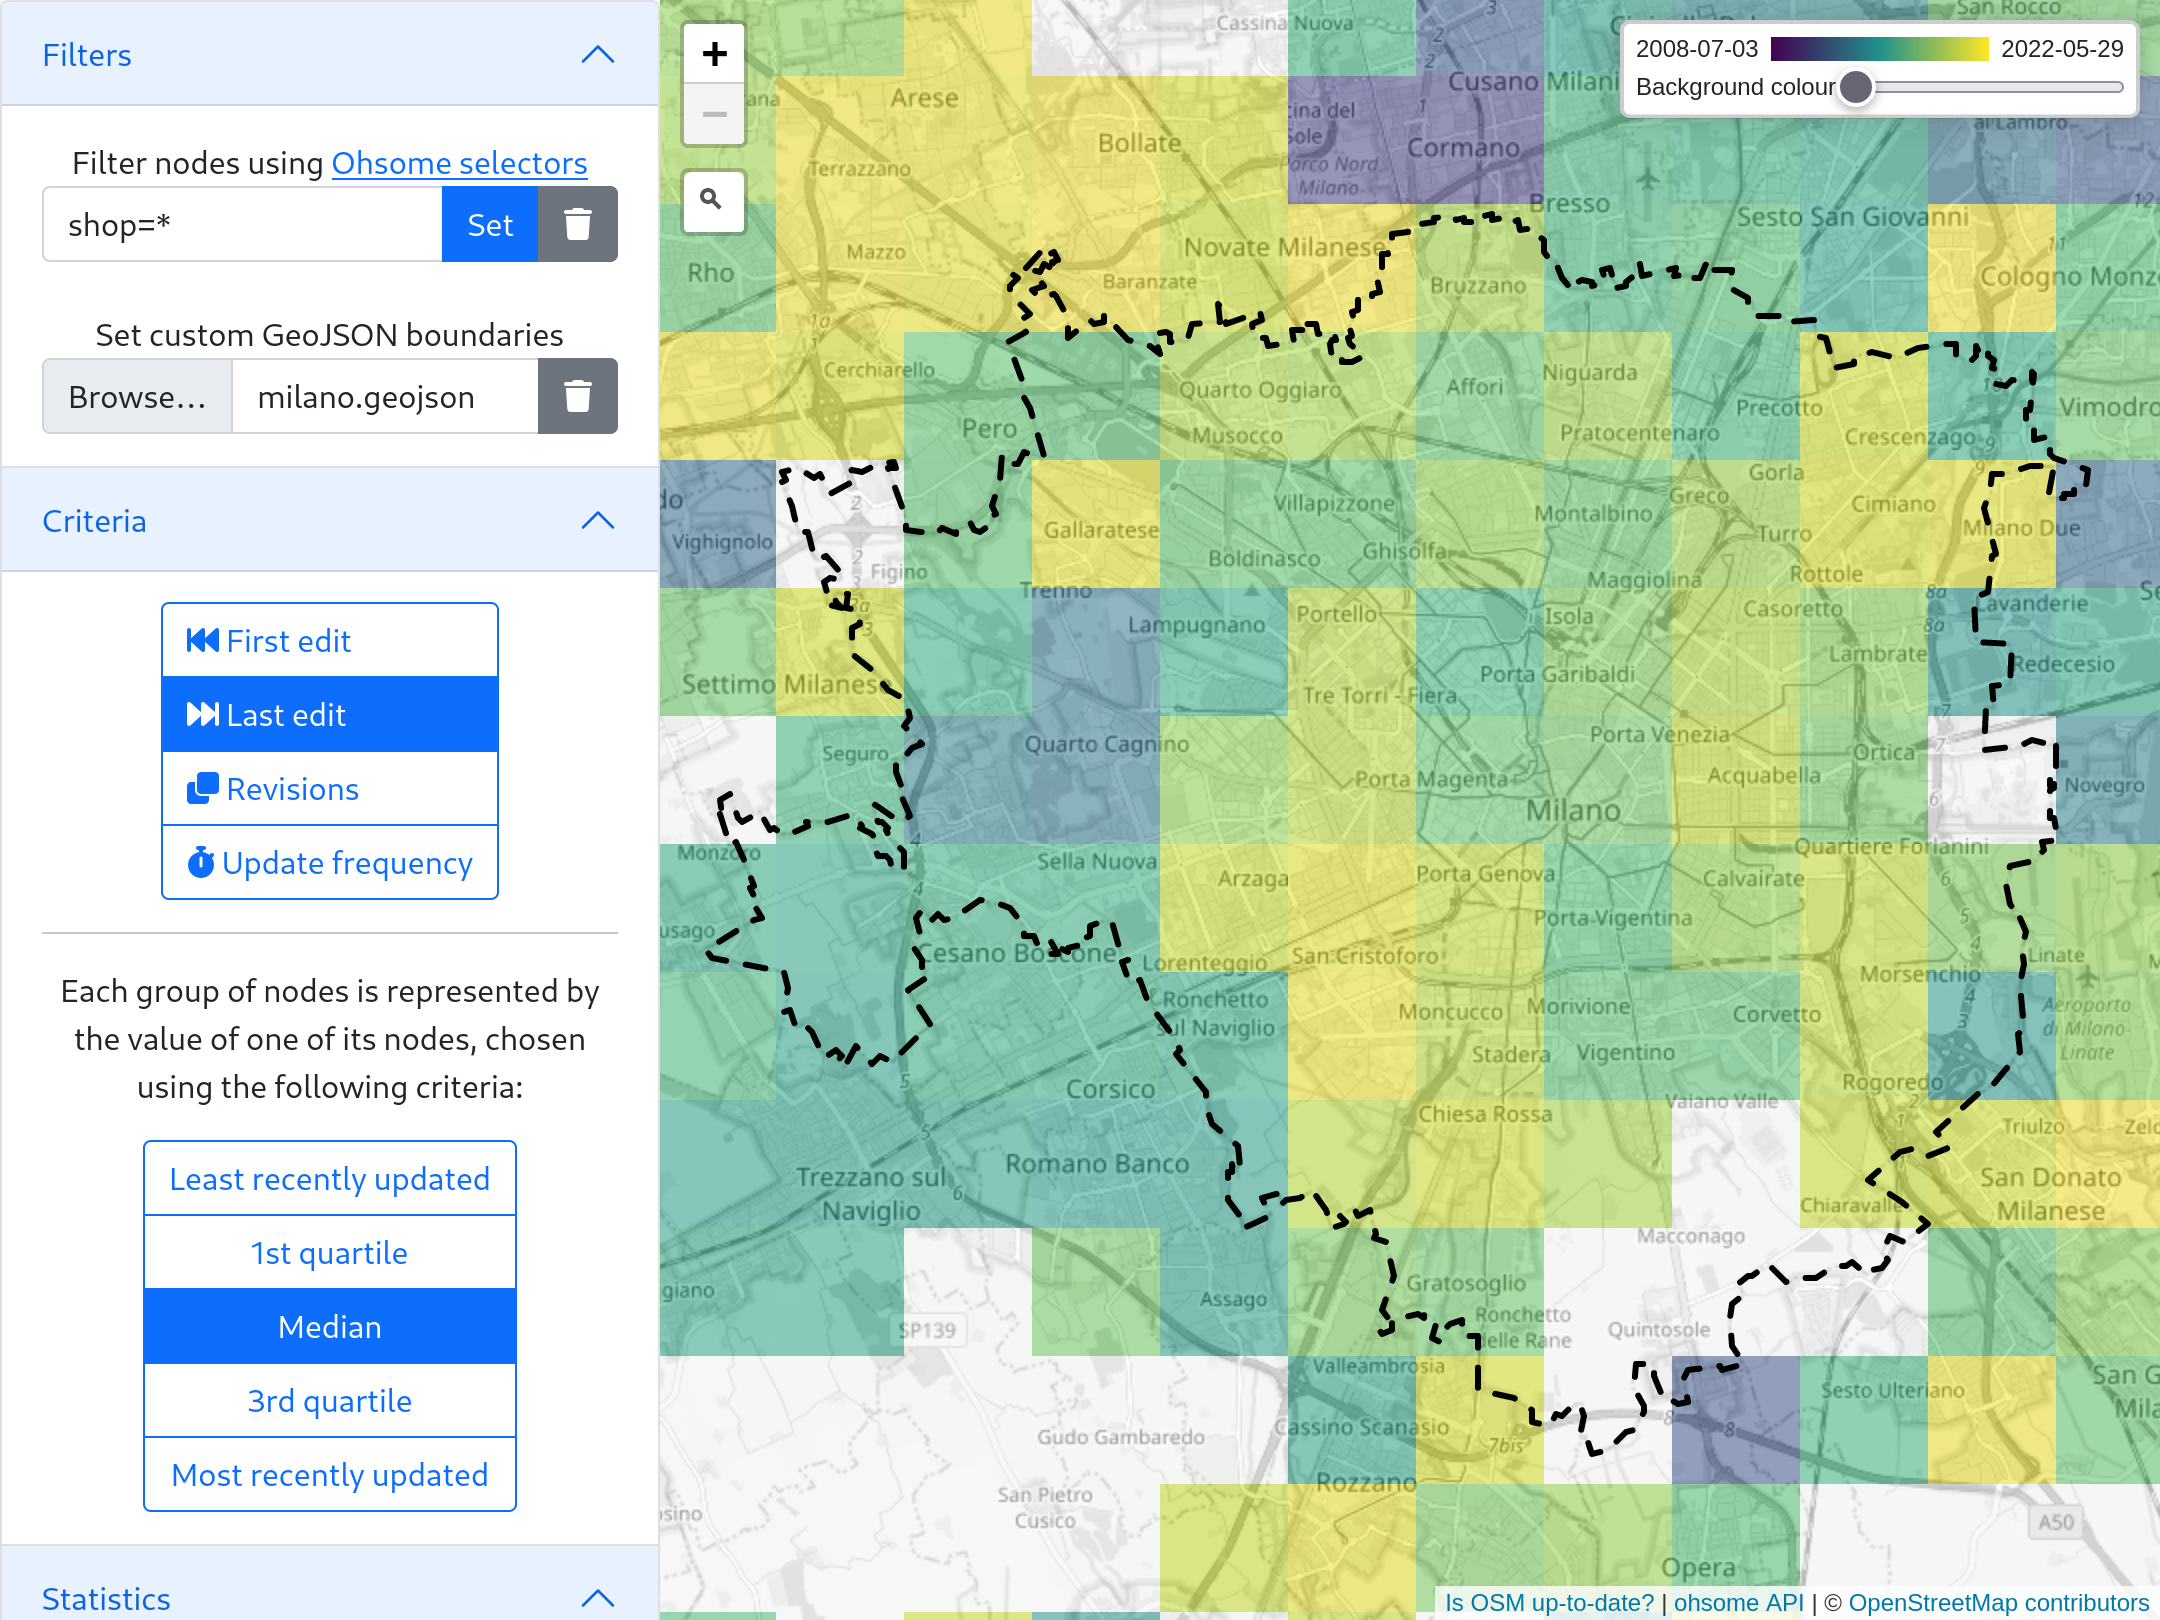
\includegraphics[width=1\textwidth]{Images/level12_milano_geojson_shops.png}
    \caption{Web app – Shops within Milano administrative boundary}
    \label{fig:level12_milano_geojson_shops}
\end{figure}

\begin{figure}[ht]
    \centering
    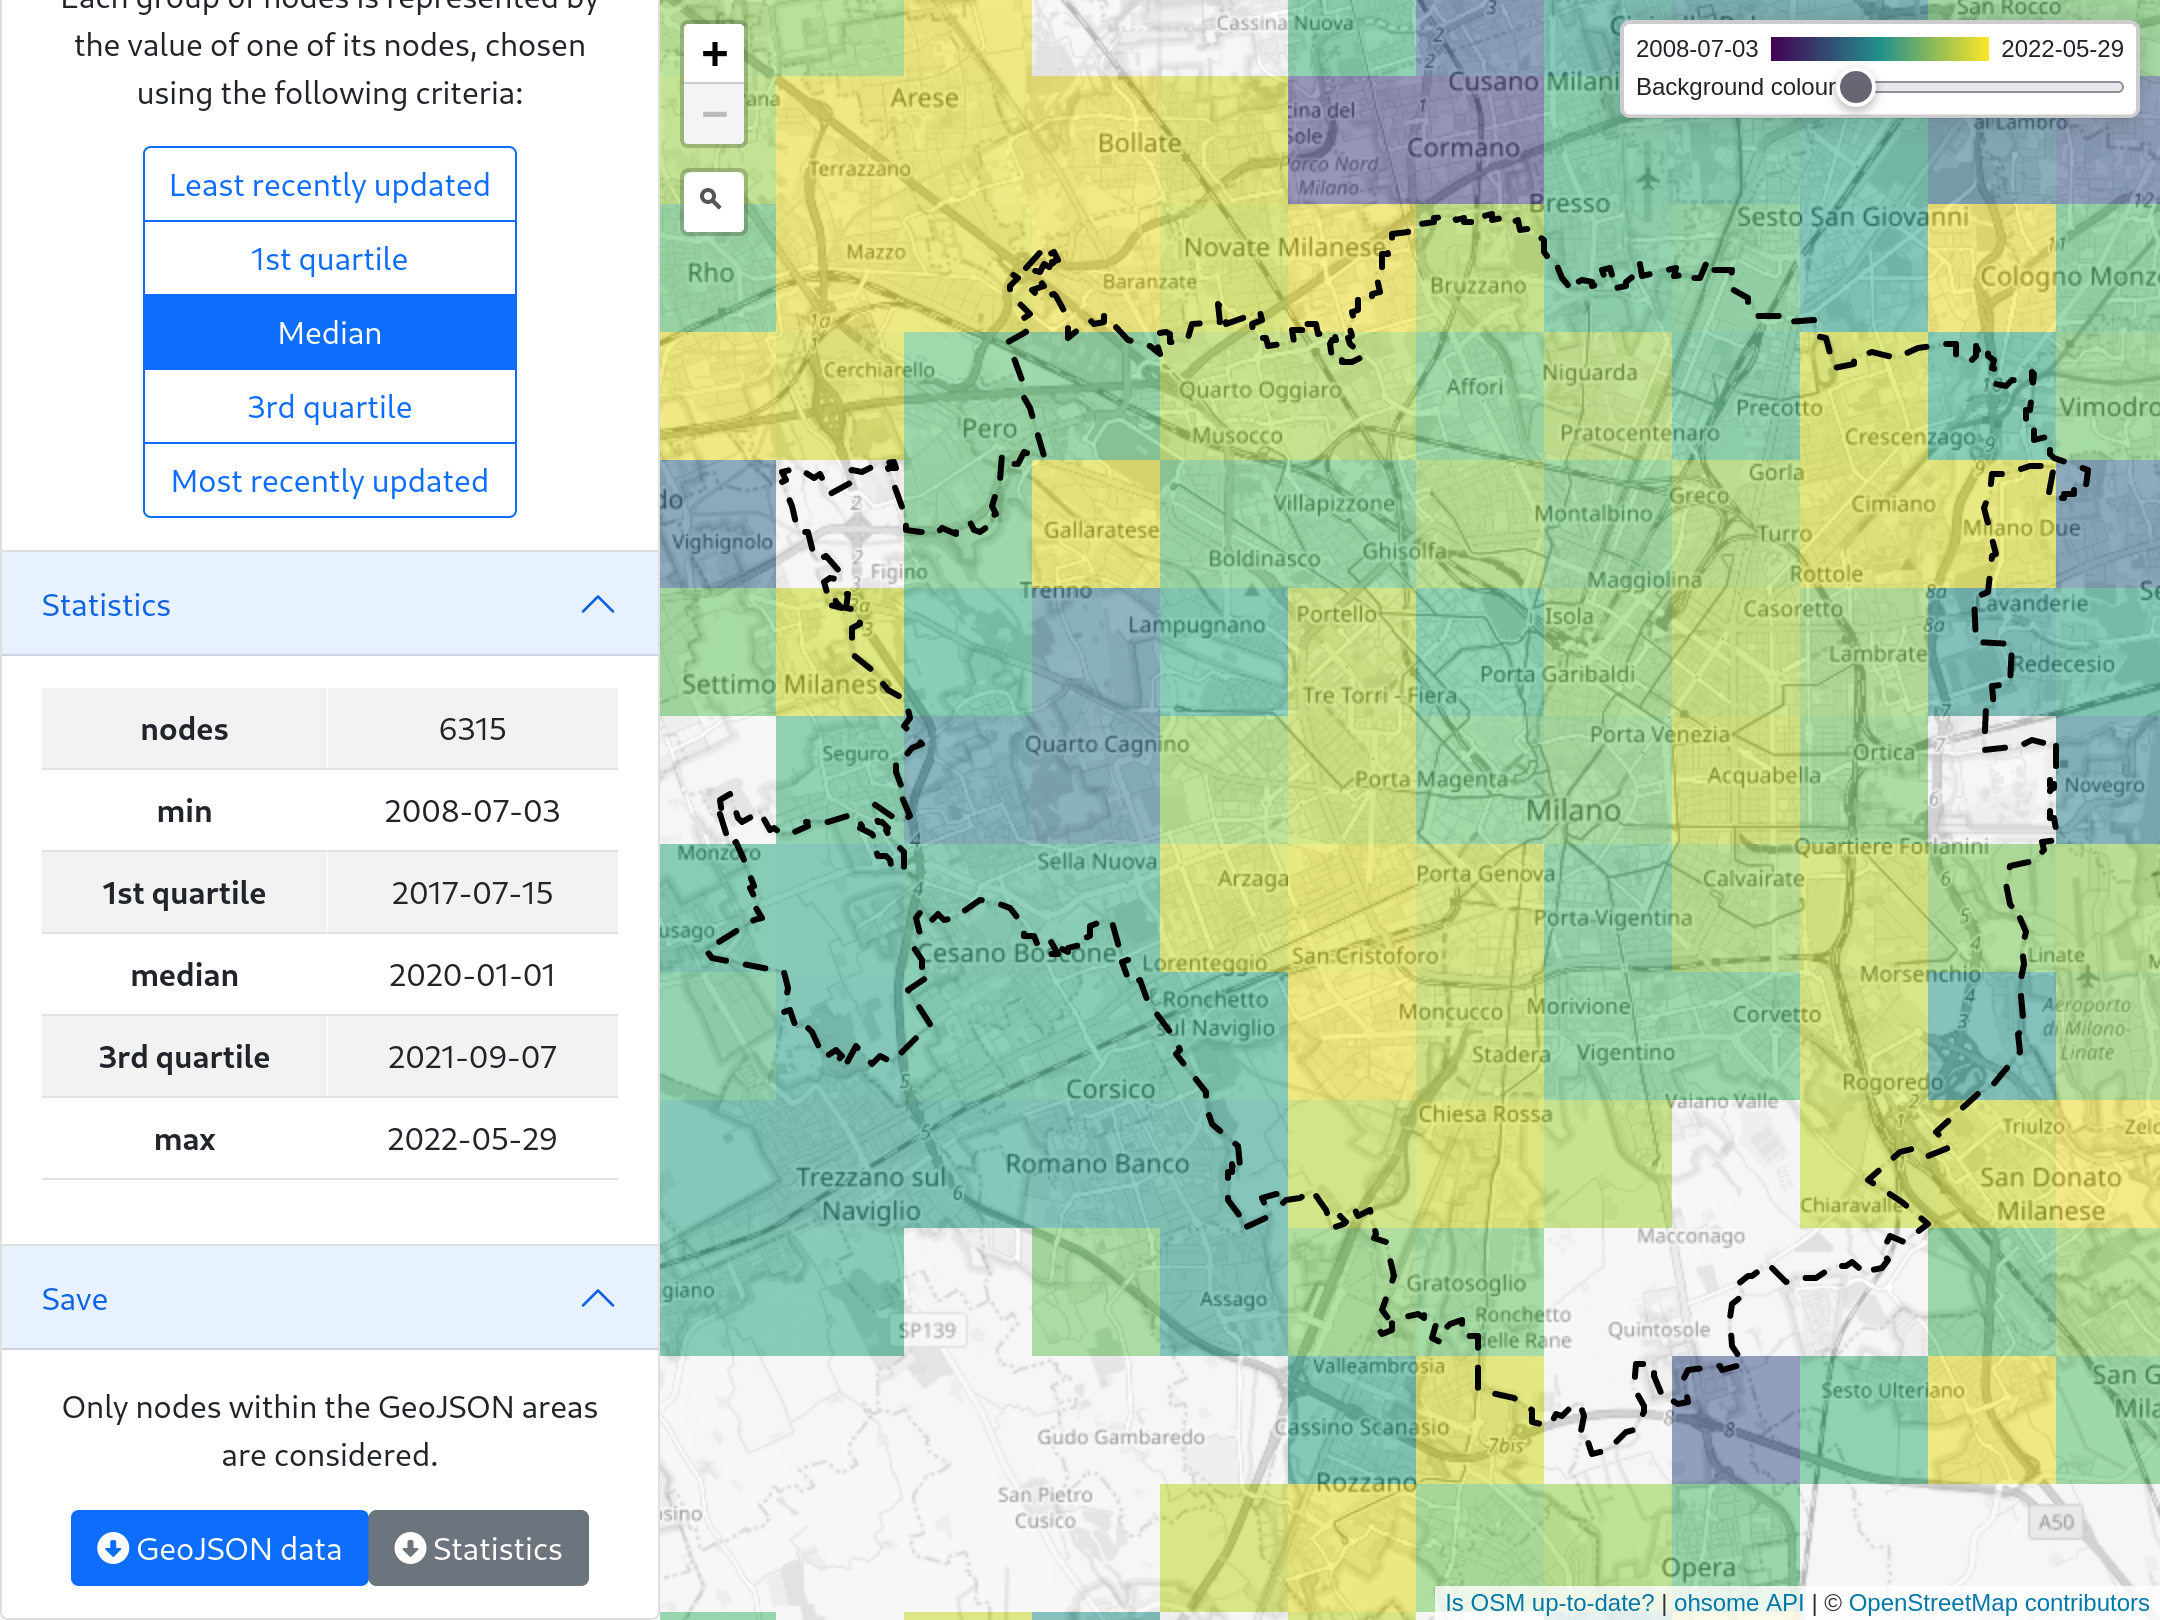
\includegraphics[width=1\textwidth]{Images/level12_milano_geojson_shops_scroll.png}
    \caption[Web app – Shops within Milano administrative boundary, scrolled down]{Web app – Shops within Milano administrative boundary, scrolled down to show Statistics and Save sections}
    \label{fig:level12_milano_geojson_shops_scroll}
\end{figure}

\subsection{Command line}

The software initially provided a command line interface (also called \textit{CLI}), in addition to the HTTP API, by relying on the Hug library. As the focus shifted more on the web capabilities of the software and Hug was posing some technical limitations (such as the inability of streamed responses, which is useful for large data transfers), the CLI has been removed, but the user can still avoid using a browser by using software like the popular curl \cite{CurlCurl2022} or wget \cite{WgetGNUProject}, or some more task-specific tool, like httpie \cite{HTTPieHumanfriendlyCLI2022}.

\noindent Here is an example of data fetching within a bounding box using httpie as client:

\begin{minipage}{\linewidth}
\begin{lstlisting}[language=bash]
$ https --download is-osm-uptodate.frafra.eu/api/getData \
    minx==9.2249536 miny==45.4767138 \
    maxx==9.2301893 maxy==45.4796778
\end{lstlisting}
\end{minipage}

\noindent Expected output (some values might differ):

%\begin{minipage}{\linewidth}
\begin{lstlisting}
HTTP/1.1 200 OK
content-disposition: attachment; filename="is-osm-uptodate_20071008T00_20220619T20.geojson"
content-type: application/json
date: Sun, 26 Jun 2022 10:54:34 GMT
fly-cache-status: MISS
fly-request-id: 01G6FTH4P52H1H51C7PTBK263Y-fra
server: Fly/9ece5bcd (2022-06-21)
transfer-encoding: chunked
via: 1.1 fly.io

Downloading to is-osm-uptodate_20071008T00_20220619T20.geojson
Done. 228.6 kB in 00:1.32045 (173.1 kB/s)
\end{lstlisting}
%\end{minipage}

\noindent Here is an example of statistics computation within a bounding box:

\begin{minipage}{\linewidth}
\begin{lstlisting}[language=bash]
$ https --download is-osm-uptodate.frafra.eu/api/getStats \
    minx==9.2249536 miny==45.4767138 \
    maxx==9.2301893 maxy==45.4796778
\end{lstlisting}
\end{minipage}

\noindent The produced file is listed below (some values might differ):

%\begin{minipage}{\linewidth}
\begin{lstlisting}[language=json]
{
    "creation": {
        "1st quartile": 1395486054.5,
        "3rd quartile": 1646904811.0,
        "max": 1655371562.0,
        "median": 1508604198.0,
        "min": 1191801600.0,
        "nodes": 1007
    },
    "frequency": {
        "1st quartile": 0.3442313737818296,
        "3rd quartile": 3.4433962264150946,
        "max": 73.0,
        "median": 0.4955872369314324,
        "min": 0.0720063128822253,
        "nodes": 1007
    },
    "lastedit": {
        "1st quartile": 1519998699.0,
        "3rd quartile": 1646904811.0,
        "max": 1655451567.0,
        "median": 1646904811.0,
        "min": 1218060291.0,
        "nodes": 1007
    },
    "revisions": {
        "1st quartile": 1.0,
        "3rd quartile": 3.0,
        "max": 22,
        "median": 2.0,
        "min": 1,
        "nodes": 1007
    }
}
\end{lstlisting}
%\end{minipage}

\subsection{GIS software}

GeoJSON is a widely used format, supported by GDAL \cite{GeoJSONGDALDocumentation}, which is used by the popular open-source GIS called QGIS \cite{QgisQGIS2022}, which supports GeoJSON. That makes it possible to open the data downloaded from the web interface, easy available on QGIS for further analysis.

Tiles can be used in QGIS too, starting from version 2.2. Such release includes safe zoom limits to prevent the server from being overloaded, a mechanism to upscale the resolution of the tiles (since QGIS interpolates the default low-resolution tiles to make them less grainy, which is an undesired mechanism in this scenario), and a brief documentation in the README file as well.

QGIS users should define a new XYZ Tile layer, with a minimum layer set to 11 and a maxim layer set to 19, and set the following URL:

\begin{lstlisting}
https://is-osm-uptodate.frafra.eu/tiles/{z}/{x}/{y}.png?upscale=512
\end{lstlisting}

The \textit{upscale} parameter is used to set the resolution of each tile, but it does not affect how many blocks the tile is divided into. This value is hardcoded, and is set to $ 8 \times 8 = 64 $.

Other parameter that can be set are:
\begin{itemize}
\item \textbf{mode}, the criteria used for the classification (default: \textit{lastedit});
\item \textbf{filter}, the Ohsome selector used to analyse some keys or values;
\item \textbf{percentile}, the percentile which should be shown when grouping nodes (default: 50; range $ [0; 100] $);
\item \textbf{scalemin}, the value associated to the coldest colour (optional);
\item \textbf{scalemax}, the value associated to the warmest colour (optional).
\end{itemize}

Every parameter is optional, including \textit{scalemin} and \textit{scalemax}, which default values are set by the server to some reasonable defaults. The \textit{getStats} function can be used to better tune these values.

\begin{figure}[H]
    \centering
    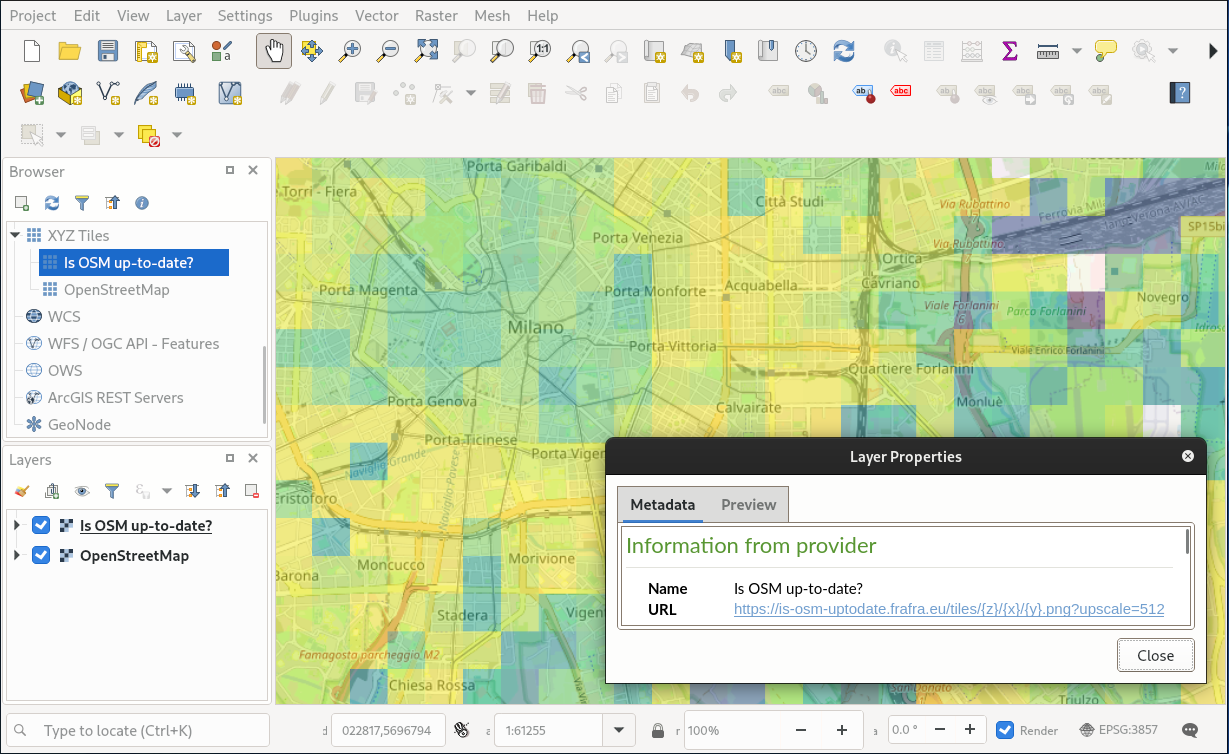
\includegraphics[width=1\textwidth]{Images/QGIS.png}
    \caption{QGIS showing \textit{Is OSM up-to-date?} tile layer}
    \label{fig:QGIS}
\end{figure}

\section{Code}

The software consists of approximately 50 files and 2300 lines of code\footnote{\Verb+cloc --vcs=git --not-match-f '[.-]lock'+}, underwent 370 revisions\footnote{\Verb+git rev-list --count v2.2.0+}, and 13 releases\footnote{\Verb+git tag | grep ^v | wc -l+}. $ \approx 8000 $ lines have been added and $ \approx 5000 $ have been deleted since the first prototype\footnote{
\Verb_git log --pretty=tformat: --numstat -- ':!:*[-.]lock*' |_\newline
\Verb_    awk '{a+=$1; d+=$2} END {print a, d}'_
}, excluding automatically generated files (such as lock files to pinpoint dependencies).

The code has been released under the AGPLv3 license \cite{GNUAfferoGeneral}, which is a copyleft license endorsed by the Free Software Foundation. AGPL licenses impose, in addition to the requirements of the popular GNU GPL license) to keep the software and its modifications open even when such software is not shipped as binary, but provided as a service.

\begin{graph}[ht]
    \centering
    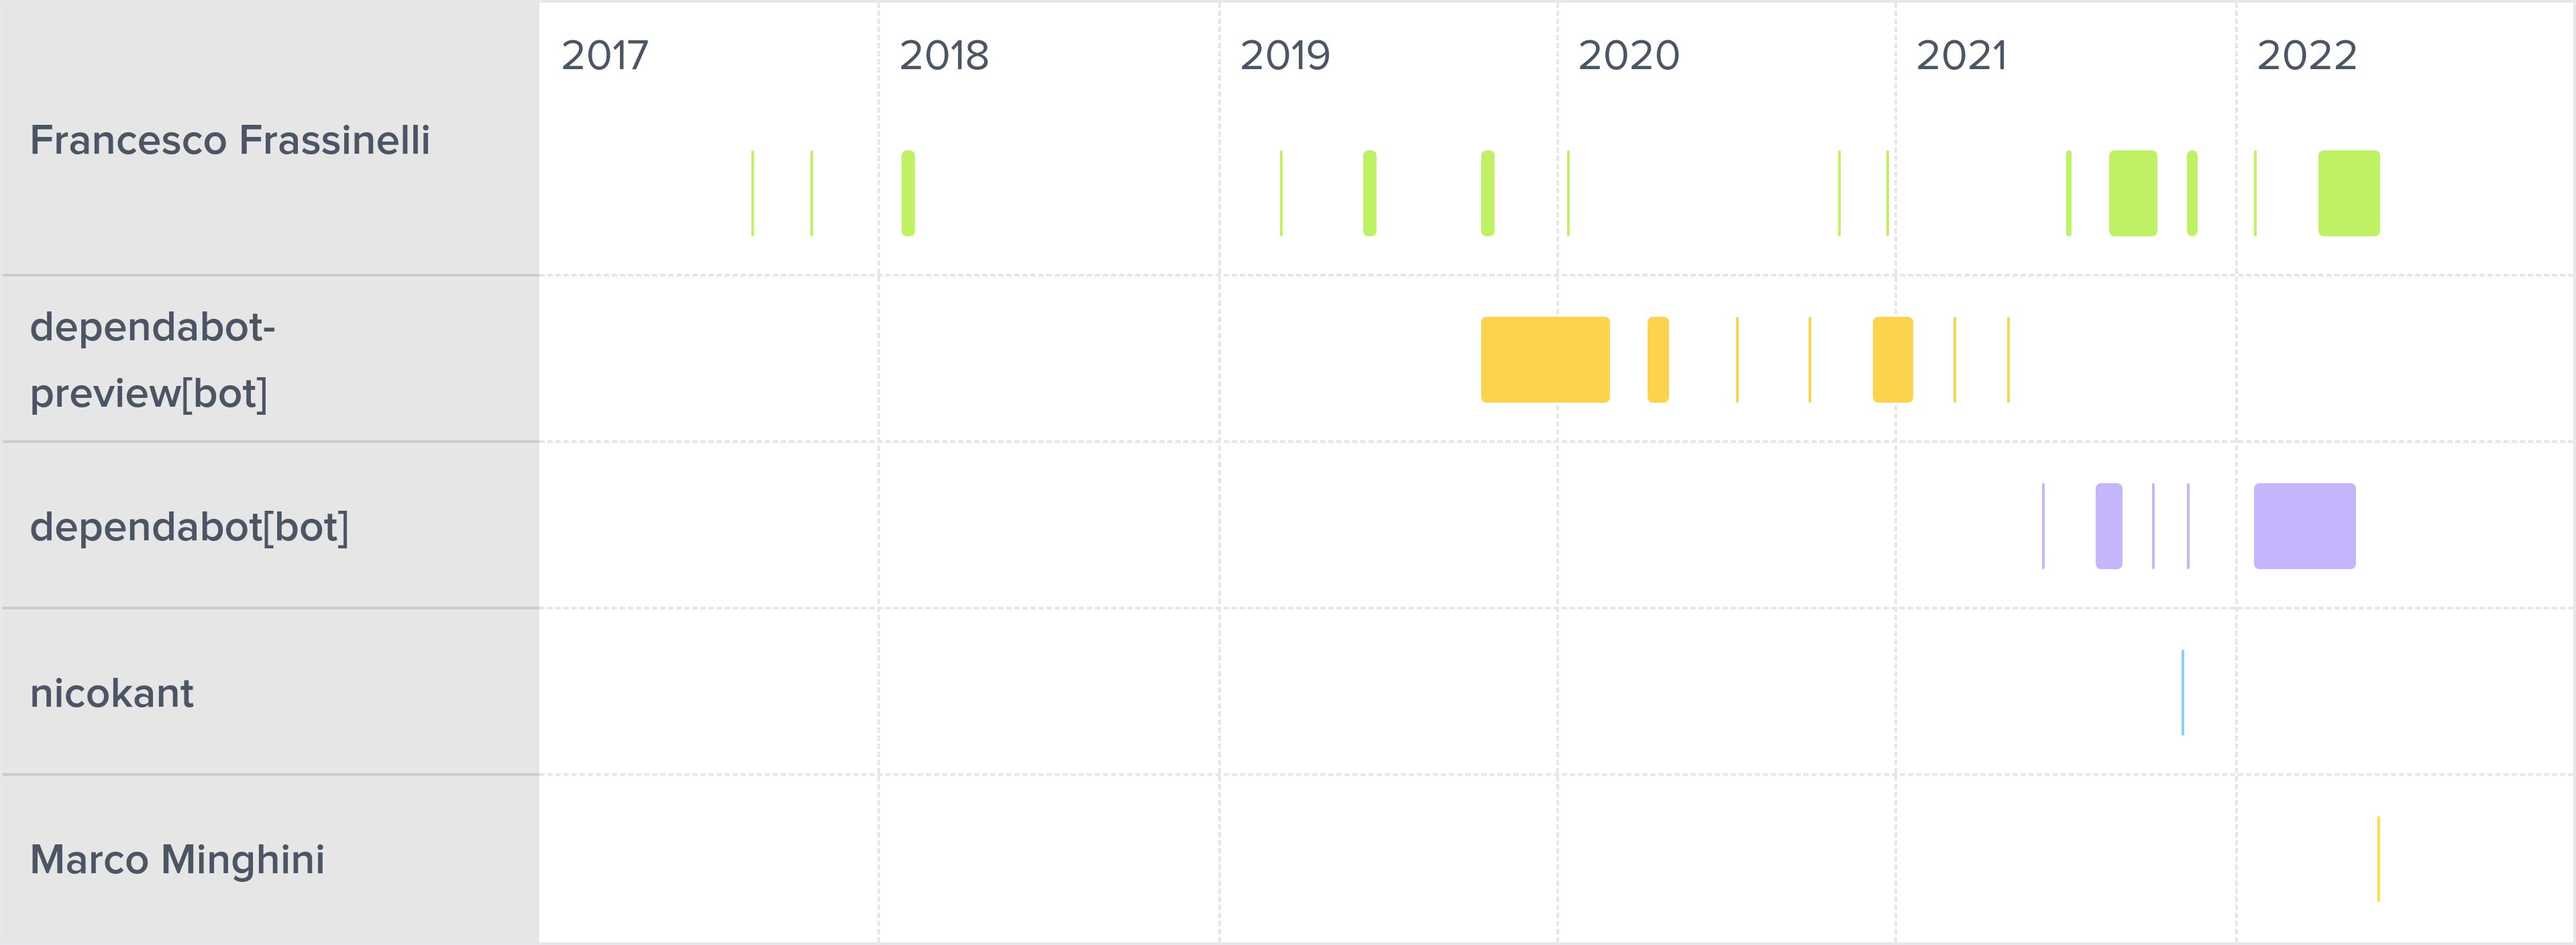
\includegraphics[width=1\textwidth]{Images/development_contributors.png}
    \caption[Development timeline]{Development timeline generated using \textit{Preceden} \cite{IsosmuptodatePreceden}}
    \label{graph:development_contributors}
\end{graph}

\begin{graph}[ht]
    \centering
    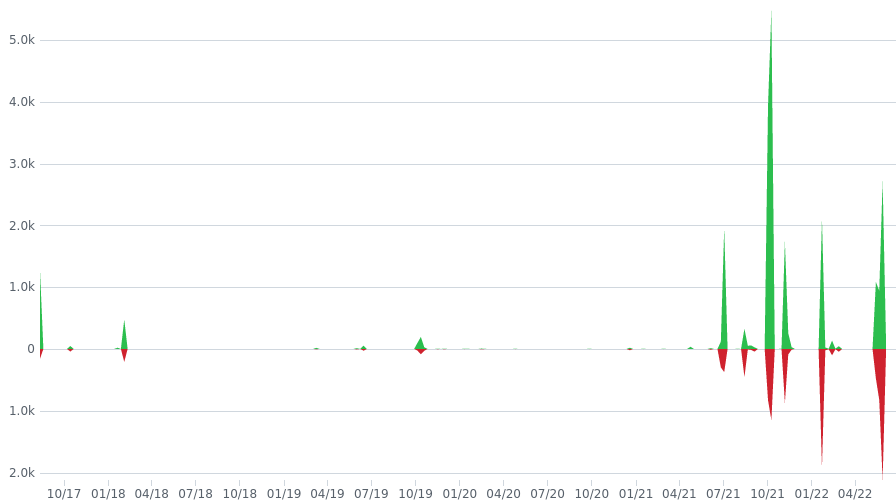
\includegraphics[width=1\textwidth]{Images/code_frequency.png}
    \caption[Line added and removed, by week]{Line added and removed, by week \cite{CommitActivityFrafra}}
    \label{graph:code_frequency}
\end{graph}

\begin{table}[ht]
    \centering
    \begin{tabular}{r|l|r|r|r}
files & language & blank & comment & code \\
\hline
9 & JavaScript & 74 & 24 & 1039 \\
14 & Python & 100 & 6 & 575 \\
5 & YAML & 13 & 16 & 206 \\
2 & Markdown & 55 & 0 & 107 \\
3 & CSS & 15 & 0 & 105 \\
3 & TOML & 24 & 3 & 97 \\
3 & JSON & 0 & 0 & 91 \\
3 & Dockerfile & 8 & 0 & 58 \\
1 & HTML & 0 & 0 & 13 \\
\hline
43 & SUM & 289 & 49 & 2291 \\
    \end{tabular}
    \caption{Lines of code, by language and type}
    \label{tab:loc}
\end{table}
% git ls-files -- '*' ':!:*[-.]lock*' | cloc --csv --list-file=- 2>/dev/null | awk -F, '{OFS=" & "} NR>4 { print $1, $2, $3, $4, $5." \\\\" }'

\subsection{GitHub repository}

The source code of such software is made available as a Git repository hosted on GitHub \cite{frassinelliOSMUptodate2022}. Two-thirds of the commits made by the main developer, Francesco Frassinelli, almost a third created by bots proposing version upgrades and triggering pipeline tests which have been manually verified and merged, and just one single commit by an external developer which extended the documentation.

The development is followed by 3 GitHub users, and the repository has been starred by 16 users.

\subsection{Code quality}

pre-commit \cite{PrecommitPrecommit2022} runs code formatting tools and checks before a commit is generated, to improve the overall code quality and consistency. In the case of \textit{Is OSM up-to-date?}, pre-commit is configured to rely on black \cite{PsfBlack2022} (the most known Python code formatter), isort \cite{PyCQAIsort2022} (which rearranges import statements) and flake8 \cite{PyCQAFlake82022} to enforce a consistent code style and respect of common Python guidelines. eslint \cite{ESLint2022} is used to maintain consistency across the JavaScript assets.

In addition to that, LGTM \cite{LGTMContinuousSecurity} is executed automatically each time new code is linked to a pull request or pushed to the repository, looking for potential code vulnerabilities and errors.

Tests are defined using \textit{pytest} \cite{PytestdevPytest2022} and \textit{seleniumbase} \cite{SeleniumbaseSeleniumBase2022} (which relies on Selenium \cite{Selenium}), to spot major regressions, both from  CircleCI \cite{ContinuousIntegrationDelivery} is used to run a pipeline executing the tests and report the results by storing logs and automatic browser screenshots as artefacts.

\subsection{Dependency management}

A proper dependency management is crucial in today software development, even in simple codebases, as a single web applications can have hundreds if not thousands of dependencies, if indirect dependencies are considered. For that reason, it is crucial to pinpoint all the dependencies with their version, to improve reproducibility and avoid regressions.

Dependencies for the frontend are reported using the common solution of \textit{package.json} for ranged dependencies and \textit{package-lock.json} for pinned dependencies, using npm \cite{NpmJavaScriptPackage2022} as package manager.

Dependencies for the backend are specified using the newer \textit{pyproject.toml} \cite{PEP621Storing} and \textit{pdm.lock} instead of the more common \textit{requirements.txt}. \textit{pdm} \cite{PDMPythonDevelopment2022} is a relatively new dependency manager for Python, which adopted some recently approved Python Enhancement Proposals (PEPs) \cite{PEP621Storing, PEP517Buildsystem} and even some that are still under evaluation \cite{PEP582Python}. One of the advantages of pdm over other mechanisms (such as \textit{Poetry} \cite{PoetryDependencyManagement2022} or \textit{pip-compile} \cite{JazzbandPiptools2022}) is its speed and the ability to take into consideration the required Python version when solving the dependencies.

In order to keep the dependencies up-to-date, the service \textit{depend-a-bot} \cite{Dependabot} has been used since the end of 2019, just after it has been acquired by GitHub in 2019, when it was still in beta.
Such service opens pull requests automatically when a new version of a library or software referenced in the repository is released. A typical pull request contains an update of the pinned version of the software, as well as a recap of the most relevant changes. This mechanism triggers the test and build pipelines, and the results of these procedures are then reported in the pull request, giving a useful and immediate insight on the potential compatibility of the proposed update.

\subsection{Docker}

Container technology\footnote{Containers are a popular method to bundle a generic application together with its dependencies, which is meant to be run in a sandboxed ephemeral environment} has been adopted early in the project, as it greatly simplify reproducibility, deployment and development of heterogeneous and complex environments, with Docker \cite{HomeDocker2022} being the most popular solution to run containers. \textit{docker compose} \cite{DockerComposeV22022}, a plugin of the CLI tool \textit{docker} \cite{DockerCLI2022}, is used to define different profiles, which cover the entire application lifecycle: development, testing and production. Being able to run containerized tests locally reduce the load on the continuous integration servers, and it is quicker, usually. Having a containerized development environment is greatly beneficial to use different Python versions and to have consistent results between development and production. The development environment is also configured with automatic reload trigger when the code change, so there is usually no need to rebuild the containers while making changes to it. Tests are defined in a different Dockerfile, so that the test container can be executed against different containers and servers.

Good practices, such as multi-stage builds, compose profiles, YAML anchors, and per-directory caching (powered by BuildKit \cite{BuildKit2022}) are used, defining a complete environment while being concise and keeping the build times and disk usage at minimum.

\subsection{Monitoring}
\label{subsec:monitoring}

Sentry \cite{ApplicationMonitoringError} is used to detect and collect errors and slow operations on both the web app and the server when the software is deployed in production. This helped to detect some corner case conditions and fix them. Such automatic mechanism is greatly beneficial, since the users are not often capable of producing high-quality bug reports with reproducible conditions, or they do not even notice minor bugs or glitches.

\section{Performances}
% jq -rc '[[.results.getData.elapsed|sort][][]] | @tsv' report_step3_rep3_fly.jsonl | tr '\t' '\n' | xargs -L6 echo

Four different areas have been chosen to measure the API endpoints perform in different scenarios. The software has been tested on a test server, which has the same technical characteristics as the one deployed in the production environment. The test environment consists of two virtual private servers on fly.io running Docker images on Firecracker. Each of them has 256 MB of RAM and a shared virtual CPU; the first hosts the main application, while the latter runs Redis \cite{RedisInternals2022}, which act as cache. Both instances run in the same datacenter, in Frankfurt, Germany. Such location is the closest to the Ohsome servers currently available\footnote{Ohsome servers are located in the area around Heidelberg and Stuttgart (Germany), within a radius of $ \SI{200}{KM} $ from Frankfurt}.

The functionalities that have been tested and timed are:
\begin{itemize}
\item \textbf{statistics} are going to be read from the \textit{/api/getStats} endpoint: it consists in a small JSON file which is transmitted after computing some basic statistics, which require the server to allocate enough memory to store all the features at once;
\item \textbf{GeoJSON} is going to be downloaded from the \textit{/api/getData} endpoint while being processed: since it contains all the features, performances can be reduced by the client network bandwidth;
\item \textbf{tiles} are going to be generated from the \textit{/tiles/\{z\}/\{x\}/\{y\}} endpoint: many requests are sent in parallel and the features, which can produce a higher load on the server, but the data being sent is actually very small: an 8 by 8 pixel PNG image.
\end{itemize}

Each endpoint has been tested with an empty cache and with an already populated cache, and each measurement is executed three times. The mean value is displayed, as well as the minimum and the maximum, both rendered in the graphs using an error bar.

Tiles have been generated with a zoom level $ z = 12 $, which is the same size used by the caching mechanism. The criteria used for the tiles is \textit{lastedit} (the default). Each tile render all the data included in its bounding box.

The software used to perform the benchmark has been published in the \textbf{benchmark} branch of the repository.

\subsection{Piazza del Duomo, Milano}

The first area is \textit{Piazza del Duomo}, in Milan. The OSM feature representing it\footnote{OSM way ID 463529462} covers an area of $ \SI{45163}{m^2} $ and contains just 152 nodes with tags.

\begin{figure}[ht]
    \centering
    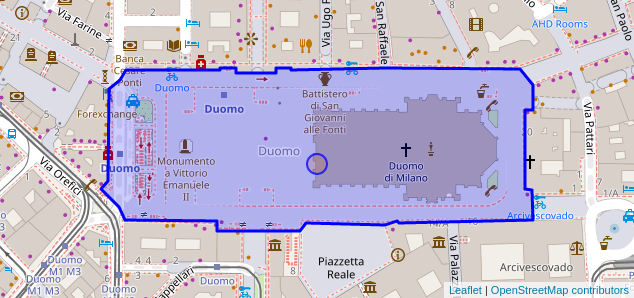
\includegraphics[width=1\textwidth]{Images/duomo.png}
    \caption{\textit{Piazza del Duomo, Milano} shown by Nominatim}
    \label{fig:duomo}
\end{figure}

\begin{filecontents}[overwrite]{\jobname-benchmark_duomo.tikz}
\benchmarkgraph{benchmarks/duomo.dat}
\end{filecontents}
\begin{graph}[H]
  \includegraphics[width=\linewidth]{\jobname-benchmark_duomo}
  \caption{Software performances for \textit{Piazza del Duomo, Milano}}
  \label{graph:benchmark_duomo}
\end{graph}

As it can be seen, there is no such of a difference between the various endpoints. The software is 7 to 8 times slower when the cache is empty, when computing the statistics or returning the nodes as a GeoJSON. This is because the area requested to Ohsome is way bigger than the one requested, to get better performance in the future requests, as it is more efficient to request a bigger area than requesting subdivision of such area.

\subsection{Municipio 1, Milano}

\textit{Municipio 1} is a subdivision of Milan, which can be considered the historical city centre. The OSM feature representing it\footnote{OSM relation ID 3952986} covers an area of $ \SI{9,4}{km^2} $ and contains $ 27547 $ nodes with tags.

\begin{figure}[ht]
    \centering
    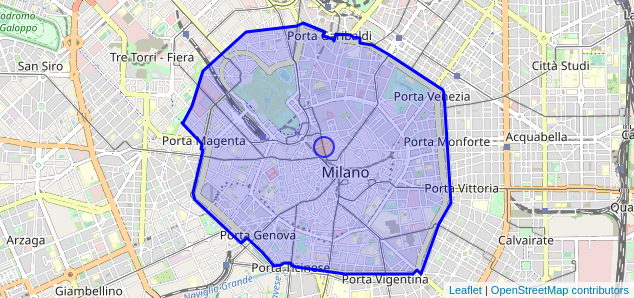
\includegraphics[width=1\textwidth]{Images/municipio1.png}
    \caption{\textit{Municipio 1, Milano} shown by Nominatim}
    \label{fig:municipio1}
\end{figure}

\begin{filecontents}[overwrite]{\jobname-benchmark_municipio1.tikz}
\benchmarkgraph{benchmarks/municipio1.dat}
\end{filecontents}
\begin{graph}[H]
  \includegraphics[width=\linewidth]{\jobname-benchmark_municipio1}
  \caption{Software performances for \textit{Municipio 1, Milano}}
  \label{graph:benchmark_municipio1}
\end{graph}

\subsection{Milano}

The OSM feature representing the \textit{city of Milan}\footnote{OSM relation ID 44915} covers an area of $ \SI{182}{km^2} $ and contains $ 149283 $ nodes with tags.

\begin{figure}[ht]
    \centering
    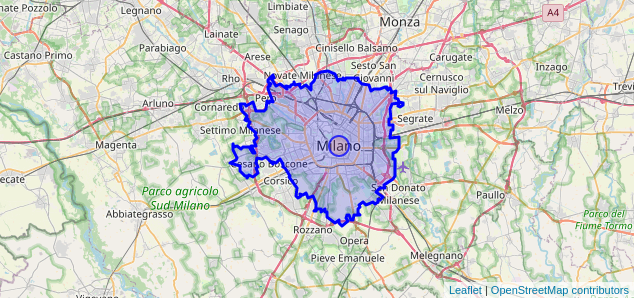
\includegraphics[width=1\textwidth]{Images/milano.png}
    \caption{\textit{Milano}, shown by Nominatim}
    \label{fig:milano}
\end{figure}

\begin{filecontents}[overwrite]{\jobname-benchmark_milano.tikz}
\benchmarkgraph{benchmarks/milano.dat}
\end{filecontents}
\begin{graph}[H]
  \includegraphics[width=\linewidth]{\jobname-benchmark_milano}
  \caption{Software performances for \textit{Milano} city}
  \label{graph:benchmark_milano}
\end{graph}

\subsection{Città Metropolitana di Milano}

The OSM feature representing \textit{Città Metropolitana di Milano}\footnote{OSM relation ID 44881}, which is an administrative boundary of level 6 in OSM, covers an area of $ \SI{1577}{km^2} $ and contains $ 334418 $ nodes with tags.

Such entity has an exclave. As a result, the boundary consists in a multipolygon, which is handled as well by the application. A quite unique peculiarity of such exclave is that it is quite far from the main polygon. The software can avoid downloading the features located between the two polygons, as they are not needed for the analysis.

\begin{figure}[ht]
    \centering
    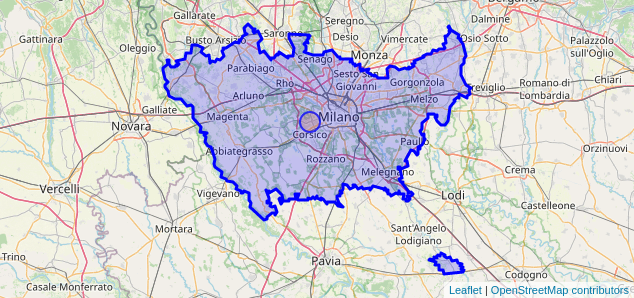
\includegraphics[width=1\textwidth]{Images/cittametropolitana.png}
    \caption{\textit{Città Metropolitana di Milano}, shown by Nominatim}
    \label{fig:cittametropolitana}
\end{figure}

During the test phase, it has been discovered that Fly.io terminates inactive connections which last more than $ \SI{60}{s} $, so this last test has been executed locally. It is still comparable to the previous tests, as differences between running the software locally or on a server have been found to be negligible for this comparison, showing that the main bottleneck is the data retrieval from Ohsome.

\begin{filecontents}[overwrite]{\jobname-benchmark_cittametropolitana.tikz}
\benchmarkgraph{benchmarks/cittametropolitana.dat}
\end{filecontents}
\begin{graph}[H]
  \includegraphics[width=\linewidth]{\jobname-benchmark_cittametropolitana}
  \caption{Software performances for \textit{Città Metropolitana di Milano}}
  \label{graph:benchmark_cittametropolitana}
\end{graph}

\section{Architecture}

The software consists of a web app, which sends requests to the backend, which relies on OpenStreetMap to provide details on specific nodes, and on Ohsome API to get historical data, which are then processed to produce statistics, tiles and GeoJSON output, where all nodes have some computed properties.

Requests to Ohsome are mediated by a caching mechanism powered by Redis, which is also used for locking, to coordinate requests to the Ohsome API across different threads, processes, or even instances.

% [rectangle, rounded corners, minimum width=3cm, minimum height=1cm,text centered, draw=black] 
\begin{graph}[H]
    \centering
    \begin{tikzpicture}[rectangle, rounded corners, node distance=4cm]
        \node (client) {Web browser};
        \node (assets) [right of=client] {Static assets};
        \node (basemap) [below left of=client] {Base map};
        \node (backend) [below of=client] {Backend};
        \node (nominatim) [below right of=client] {Nominatim};
        \node (ohsome) [below left of=backend] {Ohsome};
        \node (cache) [below of=backend] {Redis};
        \node (osm_api) [below right of=backend] {OpenStreetMap API};
        
        \path[->]
            (client) edge node {} (assets)
            (client) edge node [left] {\tiny tiles} (basemap)
            (client) edge node [fill=white] {\tiny statistics/GeoJSON/tiles} (backend)
            (client) edge node [right] {\tiny find place} (nominatim)
            (backend) edge node [left] {\tiny tiled requests} (ohsome)
            (backend) edge node [fill=white] {\tiny caching/locking} (cache)
            (backend) edge node [right] {\tiny node details} (osm_api)
        ;
    \end{tikzpicture}
    \caption{Software architecture, conceptual map}
    \label{graph:architecture}
\end{graph}

\subsection{Frontend}

The web app has been initially written as a monolithic JavaScript file, using Leaflet \cite{LeafletLeaflet2022} and Bootstrap \cite{TwbsBootstrap2022} and Font Awesome \cite{FontAwesome} are used to produce a consistent and pleasant interface

The web application has been rewritten using the popular React \cite{React2022} for version 1.8, and a complete UI redesign for version 1.9. Such choices have been made to handle the growing complexity of the interface, as well as and making it easier for other developers to approach the software in the future and contribute to it.
\textit{L.markercluster} \cite{LeafletMarkercluster2022}, with the addition of the clustering extension adapted for React named \textit{react-leaflet-markercluster} \cite{uzhvaReactLeafletMarkercluster2022}, which does not seem to be maintained at the moment, so some open bugs forced to create a forked version containing some fixes needed for \textit{Is OSM up-to-date?}, which have been proposed to be merged back \cite{IssuesYuzhvaReactleafletmarkercluster}.

Webpack \cite{Webpack2022} is used to bundle and optimize the assets, as well as for the live-reloading capabilities used during the development.

\subsection{Backend}

The software adapted aiohttp \cite{AsyncHttpClient2022} combined with gunicorn \cite{GunicornPythonWSGI}, which allowed to fetch and serve many tiles concurrently with a lower latency and resources.

To further reduce the memory usage, the software takes advantage of a streaming JSON parser called jsonslicer \cite{marakasovJsonslicerStreamJSON2022}, which relies on the fast C JSON parser YAJL \cite{hilaielLloydYajl2022}, as well as some memory-saving Python techniques as the usage of the yield statement whenever possible.

The mercantile \cite{Mercantile2022} library is used to compute tiles and the bounding boxes for cached data, while pygeos and shapely have been added in version 2.2 to handle arbitrary GeoJSON boundaries.

GeoJSON boundaries are parsed and applied using Shapely \cite{Shapely2022} and PyGEOS \cite{PyGEOS2022}.

\subsection{Caching}

Caching the response to arbitrary bounding box requests makes caching useless, as each of the requests can have a different bounding box, even if slightly. To address this issue, each bounding box is normalized into a set of one or more bounding boxes belonging to a known grid, which is defined as a standard regular tile grid at a specific zoom level.
Each of the resulting bounding box tiles are encoded as quadkey \cite{rbrundrittBingMapsTile}, which is an efficient method to encode a tile using a single number. Quadkeys has also been chosen as fetching a tile composed by many can be done by requesting all the tiles that share as prefix the quadkey of the wider tile\footnote{For example, the data of the tile having 124 as quadkey can be computed by aggregating the data of tiles starting with 1; the list of these tiles can be obtained by executing \verb+KEYS 124*+  in Redis}.

The software then checks if the desired areas as already been cached by looking at the Redis database. If the data is not there, a lock is created on the tile, to signal that the tile is in the process of being requested to the Ohsome API, so other requests of the same tiles are going to wait, and duplicate requests are avoided; the software then stores the results and removes the lock so that all requests can be satisfied. If the data is in the cache, there is no need to fetch data or to use locks. The access to Redis is mediated by walrus \cite{leiferColeiferWalrus2022}, which provides some useful abstraction and safety, like its locking mechanism.

Each tile has a TTL (Time-To-Live) of a month, before it gets discarded automatically. To prevent the cache from getting full, a soft-limit of $ \SI{800}{MB} $ is enforced using a LFU (Least Frequently Used) policy, so that when such limit is reached, Redis stats to automatically drop the least popular tiles. This mechanism has proved to be very effective and flexible to different setups, as the software can easily take advantage of the available memory of the system.

Redis also has some spatial capabilities, but they are not considered to be useful, since no TTL or cache eviction policy can be specified on the members of a geometry set. 

\section{Limitations}

\subsection{Area of study}

The web app is locked on a minimum zoom level of $ 12 $ due to performance limitations, which means that the tiles are loaded with $ z = 11 $; such limit is also enforced for requests coming from other clients (such as GIS software). It is possible to use the \textit{getData} for wider areas, thanks to its streaming capabilities, but it has not been extensively tested. \textit{getStats} could take too much time to start giving a reply (since it needs to load all the data first) and the connection could be terminated before the computation ends, while using too much memory on the server.

\subsection{Relation to GIS software}

The web app is not a full-fledged GIS software, nor it aims to be one. Its features are limited to the scope of evaluating OSM uptodateness. There is also the risk of wasting time and resources by trying to reimplement features already available on popular GIS solutions. This is the reason GeoJSON and web tiles has been used: to provide standard interfaces that could be used by external tools. The integration with GIS software is limited and could be greatly improved.

\chapter{Reception from the community}
\label{ch:reception_from_the_community}

A survey targeting version 2.2 \cite{SurveySondaggioFrafra} has been shared with people involved with OpenStreetMap (both mapping and research activities), to evaluate how the software is perceived and if it is considered useful. It has been asked to test the software first and fill the form afterwards. The survey has been made available in both English and Italian. Instead of sharing a direct link to the survey, a dedicated wiki page on the GitHub repository has been created, which contains the links to the survey in both languages and their results.

The software used for the survey is \textit{CryptPad} \cite{CryptPad2022}, an open-source web application focused on user privacy, with end-to-end encryption.

The survey has been shared within the following communities:
\begin{itemize}
\item @OpenStreetMapItalia group chat on Telegram;
\item @Polimappers group chat on Telegram;
\item science@openstreetmap.org mailing list;
\item talk-it@openstreetma.org mailing list.
\end{itemize}

The survey has also been shared by some users on Twitter and by email.

All the answers provided in Italian have been translated to English for consistency.

\section{Respondents}

23 people filled the form, and they replied to the question “\textit{Which user case fits you the most?}” (which allowed multiple answers) by describing themselves as OSM contributor in 16 cases, researchers or students in 5 cases and just one as user. 2 selected the option "\textit{Other}". 

\section{Features}

It has been asked to each respondent to give a score for each feature, ranging from \textit{terrible} to \textit{great}, using \textit{bad}, \textit{average}, and \textit{good} as intermediate options. The question has been formulated as the following: “\textit{How would you rate these features of is-osm-uptodate?}”.

Two users replied with a different scale, using stars instead of text, from 1 (minimum) to 5 (maximum). It has been found that a user gave almost exclusively 1 and 2 stars, while still providing a positive final overall comment on the solution. It has been assumed that the question has been misunderstood, as the user could have it interpreted as a request of rating the features based on their importance, not on how bad or well they have been implemented, or the user could be not familiar with the paradigm of the stars as paradigm to express a vote.
The scores given by such user have been ignored in this section, and the survey has been improved to avoid this potential confusion, by using textual labels.

Few other responses have been excluded, as a user wrote: “\textit{My “terrible” answers above can be ignored. I did not try, so I needed a “no idea” option}”. The software used for the survey allow seeing non-aggregated data, which made it possible to fix the results as requested.

\pgfplotstableread[
    col sep=tab,
]{survey/features.dat}\featurestables

\begin{filecontents}[overwrite]{\jobname-survey_features.tikz}
\begin{tikzpicture}
\begin{axis}[
    ytick={data},
    yticklabels from table=\featurestables{Question},
    xbar,
    xmin=0,
    xmax=100,
    xtick distance=10,
    xtick pos=both,
    xticklabel={\pgfmathprintnumber{\tick}\%},
    xmajorgrids=true,
    height=15cm,
    bar width=22pt,
    y dir=reverse,
    bar shift=0pt,
    legend style={at={(0.5,-0.1)},anchor=north},
    reverse legend,
    legend columns=5,
]
\addplot+ [
    black,
    fill=clr5!,
] table [
    y=Index,
    x=Terrible,
    col sep=tab,
] {\featurestables};
\addplot+ [
    black,
    fill=clr4!,
] table [
    y=Index,
    x=Bad,
] {\featurestables};
\addplot+ [
    black,
    fill=clr3!,
] table [
    y=Index,
    x=Average,
] {\featurestables};
\addplot+ [
    black,
    fill=clr2!,
] table [
    y=Index,
    x=Good,
] {\featurestables};
\addplot+ [
    black,
    fill=clr1!,
] table [
    y=Index,
    x=Great,
] {\featurestables};
\legend{Terrible,Bad,Average,Good,Great}
\end{axis}
\end{tikzpicture}
\end{filecontents}

\begin{graph}
  \includegraphics[width=\linewidth]{\jobname-survey_features}
  \caption{Scores users gave to each feature}
  \label{graph:survey_features}
\end{graph}

\subsubsection{Easy to use}

The software seems relatively easy to use for most of the user, which can be a good result for such a usual software, with some unique patterns of interactions, but there is still room for improvements.

\subsubsection{Processing speed}

The processing speed seems to be the area where the software got the worst scores. This could be due to different reasons:

\begin{enumerate}
\item Two \textit{terrible} votes have been cast while the software was experiencing a technical issue: the Redis database has been unreachable by the main application, which has no retry mechanism, since it has not been taken into account connectivity issues. Such a scenario has never been seen before, as both services have been executed on the same machine, in an ordered manner. \textit{fly.io}, which is the service that has been recently used to deploy the application, starts two virtual machines independently of their statuses or availability. A restart of the Redis database could cause a network failure. The mechanism to restart containers based on health checks failed too. The services have been restarted manually few days after.
\item Some users tried to reach a location by dragging the map around repeatedly instead of using the search function, which results in a lot of calls to the server and higher waiting times. Previous versions of the software did not load the data on each boundary change, but they relied on a button to fetch the data. This is an effective method to avoid loading unnecessary data, but it reduces the usability of the platform. A potential solution could be to revert to the previous behaviour and adding a keyboard shortcut for users that needs to fetch data repeatedly, as well as some mechanism to avoid loading new tiles automatically.
\item Some users could have very high expectations on how quickly such a system could be able to fetch and process the data, even if the solution is based on Ohsome (which is the fastest public API for fetching historical OSM data) and it can be even noticeably faster than it when the data has been cached.
\end{enumerate}

\subsubsection{Parameters and filters}

Parameters and filters seems relatively good, but the service disruption could have had an effect on this question too. Even when excluding the worst score, it looks like a user does not feel comfortable enough with the given filters. It could be due to not being familiar with the concept such quantiles, or by the syntax used by Ohsome to specify tag filters. A help text with a link has been added afterwards, but the interface could be further improved to assist the user in defining tags.

\subsubsection{GeoJSON download}

The mechanism to download the data as GeoJSON is rather simple: the user needs to click a button and the download starts immediately. This simple question further suggest that the outlier could be due to a temporary and technical fault of the solution which affected almost all of its functionalities.

\subsubsection{Statistics}

Statistics got a good score. They are consistent with the criteria, and they can be downloaded too, which seems what the users expected by a relatively simple, yet important, functionality.

\subsubsection{Search function}

The search functionality relies on a very common Leaflet widget, so the results were in line with the expectations.

One user gave the lowest score possible, but such user could not find the search button. Other users had the same problem, so the appearance of the search widget should be changed.

\subsubsection{Clustering/grouping}

The clustering/grouping feature received a good score, which seems to confirm the development direction taken during the last year. The \textit{bad} vote could be due to suboptimal performances (some mobile devices can lag when using the clustering feature on many nodes) or to a not-so-intuitive subdivision of the areas containing the clustered nodes (such areas are visible only when hovering the mouse over a clustered node). These areas could be made visible all the time or a Vonoroi diagram (consistent with the clustering method) could be generated and shown as an additional layer, to better represent how the space is subdivided. The \textit{terrible} vote could be linked to bad performances on some low powered devices, such as smartphones.

\subsubsection{Tiles}

What could be considered as the best result came with the last question, which shows that the recent addition of the tiles as a method to aggregate data has proven to be an effective and intuitive method. Tiles received less average and negative votes compared to the usual clustering.

Such a final result suggests that regular tiling should be considered as the main (and potentially the only) method to group nodes.

\section{General questions}

Almost half of the respondents have used the software before. All of them agreed that the software improved recently.

\begin{graph}[H]
  \surveygraph{43/Yes, 9/I don't recall, 48/No}{clr7!,clr8!,clr6!}
  \caption{Survey – Have you tried it before?}
  \label{graph:survey_first_time}
\end{graph}

\begin{graph}[H]
  \surveygraph{40/Yes; a lot, 60/Yes; a bit}{clr1!,clr2!}
  \caption{Survey – Do you think it has been improved recently?}
  \label{graph:survey_improved}
\end{graph}

“\textit{No; it is slightly worse}” or “\textit{No; it got a lot worse}” have not been selected by anyone.

It has then been asked to the respondents if they like the software, if they intend using it in the future, and for which purpose.

\begin{graph}[H]
  \surveygraph{18/Very useful, 74/Quite useful, 4/Not so useful, 4/Useless; I am not interested}{clr1!,clr2!,clr3!,clr4!}
  \caption{Survey – Is it useful?}
  \label{graph:survey_useful}
\end{graph}

No one replied “\textit{Useless; I'd rather rely on other tools or services}”.
Such result could be considered as a final score on the software, which is a positive one. One user is not interested in the software, but is not willing to consider other solutions, which could hint at the fact that such user is not the target of \textit{Is OSM up-to-date}.

\begin{graph}[H]
  \surveygraph{57/Yes, 39/Maybe, 4/No}{clr1!,clr3!,clr5!}
  \caption{Survey – Would you use it in the future?}
  \label{graph:survey_future_use}
\end{graph}

Respondents are almost equally split between the ones that are going to use the software again, and the ones that are not sure about that. The only negative result came from the user that is not interested at all in this kind of tools.
Improving the most critical aspects that have been highlighted in the survey could increase the user retention and make the software more popular in the community.

\section{Possible usages}

The respondents would use the software for improving OpenStreetMap data in 13 cases (it is reasonable to assume that these users would do data gardening, mostly), and for doing research or analysis in 8 cases. 2 respondents also checked the option "\textit{Other}", suggesting other ways to use the tool. Multiple choices were allowed.

Just 2 respondents that did not qualify themselves as researchers or students, replied to the question “\textit{For which purposes are you going to use it?}” suggesting that the software could be interesting to explain “\textit{[…] OSM data quality to potential users}” and to check “\textit{[…] the contribution trend in my interest area}”.

Almost all respondents that qualify themselves as researchers or students, replied to the question “\textit{Which kind of research or analysis are you thinking to do with it?}”.

\subsection{Practical applications}

A first group of answers have in common the focus on figuring out which areas need to be mapped or updated first:
\begin{itemize}
\item “\textit{Combine with data from Disaster Ninja to get \underline{prioritize} area to map.}”
\item “\textit{Research on \underline{prioritization} of areas or types of elements in updating information in OSM. Connection between presence of users (and how many or expert/new) and frequency of updates.}”
\item “\textit{\underline{Automatic identification} of areas where OSM might need updates}”
\end{itemize}

Another answer is still focused on practical applications, but more on monitoring instead of mapping: “\textit{[…] I am thinking about a \underline{rapid data quality monitoring} tool of critical infrastructures in global south, where the OSM contributions are intensive and quickly updated}”.

Having researchers considering the tool in such scenarios is a valuable feedback, suggesting that the software could have a positive impact on various areas of the world, especially if further improved.

%\subsection{General research projects}

A smaller group of answers is more focused on the research aspects:

\begin{itemize}
\item “\textit{As an academic project to \underline{quantify various statements} made on the use and validity of OSM}”
\item “\textit{Data \underline{quality analysis}, extent of interaction with the data}”
\end{itemize}

One respondent, instead, is going to “\textit{[use] this for \underline{student assignments}.}”.

These answers hint that the software could be used as starting point for future research projects regarding OpenStreetMap temporal accuracy and up-to-dateness.

\section{Additional comments}
\label{sc:additional_comments}

Some respondents left a final comment, that could be worth discussing.

Comments are mostly exclusively positive, such as “\textit{great tool!}”, “\textit{Great work, congratulations!}” and similar, or more articulated ones, like “\textit{Definitely a nice attempt to explore OSM intrinsic data indicators}”, or “\textit{this is an interesting tool and I think it can be useful for both mappers and data users!}”.

Various users noticed technical issues, glitches or difficulties in using the interface. For example, some of them failed to spot the search icon to find and move to the desired location, or they triggered the loading of so many data during their movements on the map that the load times grew too much.
Most of the discovered limitations were known already, but it has been valuable to know which ones have been hit the users the most and how.

Some improvements have been suggested, such as:
\begin{itemize}
    \item remove the restriction on the minimum zoom level while avoiding the tile loading on even wider areas: that would allow users to roam freely around the globe, without having to rely on the search function;
    \item store the last location in a cookie, instead of the URL, so that the user would always land on the last visited location;
    \item allow setting a different colour range;
    \item add information about the software and how to use it within the application itself;
    \item show tag filters in the legend;
    \item hide the grouping criteria when data is not grouped;
    \item add tags data to the downloaded file;
    \item analyse ways too.
\end{itemize}

Just the last two suggestions would require a major change in how the software works, since more data would need to be fetched and the system would become too slow. This feature would then need to found an even better mechanism than fetching data from Ohsome APIs.

A discussion started on the Italian OSM mailing list called \textit{talk-it} \cite{frassinelliTalkitOSMUptodate2022}. 5 users wrote different comments and consideration that were not in the result of the survey.
Reaction were mixed: some users are puzzled by the software and its goals, and they would probably benefit from having a global quality index related to temporal accuracy, while others were very happy about the tools, or interested, and found it useful.
One of them also mentioned the \textit{check\_date} tag \cite{KeyCheckDate}, which can be used to specify when a feature has been checked, thus having a better understanding if a node hasn't been changed for a while because there was no need to update it or if it has been neglected. Such tag is not widely used \cite{CheckDateKeys}, and in case contributors start to use it more often, the software would still register a change of such tag as a new revision, thus improving its metric without any further change.

\chapter{Conclusions}
\label{ch:conclusions}

\section{Final considerations}

\textit{Is OSM-up-to-date?} proposes a new solution to analyse OSM history, providing to both contributors and researchers an additional tool with unique features to explore the data and perform their tasks, thus moving forward the estimation of the temporal intrinsic quality of OSM data.

The development of the software posed major difficulties, especially when moving from a working prototype to a production solution that could work efficiently on areas that are 3 orders of magnitude bigger, requiring to change the software stack multiple times, evaluating different approaches. However, the work proved that it is possible to run historical analysis on OSM data using modest resources within minutes across hundreds of thousands of nodes. Working on it and exploring different technical methods provided new insights on how this class of problems can be tackled.

The presentation of the intermediate results at different conferences and to the OSM communities resulted in interesting feedback and opportunities for improvement. Writing papers on the matter required to have a better understanding about the state of the art on the topic and brought the research to adhere to higher quality standards.

The feedback from the community has been mostly positive. In addition to the many OSM contributors interested in data gardening who found the tool interesting, there is an interest in the academic environment to use the software for scientific purposes. The technical evaluations, benchmarks, and trials made during its development could be considered a starting point for implementing more sophisticated solutions that could be even more appealing for a research-focused audience. The hope is that the research in this field can further progress and quality indexes for intrinsic temporal accuracy can be defined so that they can be implemented in \textit{Is OSM up-to-date?} and other software.

As a final result of this research and development process, a list of future work and research activities that could be done is shown in the following section.

\section{Future work}

\subsection{Research topics}

\subsubsection{Overall quality index}

This is probably the most important goal that is left from a research perspective: finding a formula or a method that could provide a quantitative estimation on the temporal accuracy of the OSM data, that goes beyond the computation of the average update frequency, last edit or number of revisions, capable of taking into account  tag classes and calibrating the result based on spatial trends.

\subsection{Features}

\subsubsection{Improved usability}

Usability would greatly benefit from the changes proposed by the respondents to the survey (see \ref{sc:additional_comments}).
Users' feedback demonstrated that it is crucial to find a different way to let the user search for a specific location. A horizontal bar to type the location could be used, but it would clash with the legend in the top-right corner on smaller screens; a set of CSS rules could be made to avoid such an issue.

Other improvements that have been proposed are linked to the map handling as well, like giving the user the freedom to zoom out as much as needed, without any limit, or store the last visited location.

\subsubsection{Custom boundary for tiles}

It is not possible to specify a custom GeoJSON boundary for tiles, which are always rendered without applying any spatial filter on the tags. It could be useful to crop data based on the boundary before computing the tile, but users could be puzzled when seeing non-transparent pixels placed over a boundary line: how would it be understood? The user might ask if the software has taken into consideration features just across the boundary as well.
This problem has been solved when producing hexagonal maps on QGIS by cropping the hexagons using the boundaries, which seems the optimal solution that should be implemented in the new software as well, but tiles are raster data, not vector, so a different API should be developed to produce vector tile-like data.
Another solution would be to upscale the raster before cropping it to match the boundary so that it would be less noticeable to the user that the graphical representation of the tile does entirely match with the boundary.

\subsubsection{Export area as GeoTIFF}

The software allows to download statistics and a GeoJSON representing all the features with their computed properties, but it does not allow to download a single GeoTIFF file of the area under analysis. While the tile layer allows having such a functionality outside of the software, by relying on specific tools or extensions to GIS software, providing to the user a single button would greatly improve the user experience. 

Such improvement would greatly benefit from the possibility to use custom boundaries on tiles.

\subsubsection{Better error handling}

The server catches various exceptions, but the current user interface lacks the capability to display errors in a meaningful way to the user. The service Sentry (see \ref{subsec:monitoring}) highlighted some rare errors as well, such as cache locking failures related to unexpected reboots or timeouts. Various errors are also triggered by the fact that the software relies on external services, which are not always available; users could attribute the cause of the issue they might experience to the software instead of the external API in some cases.

\subsubsection{Better GIS integration}

Another potential improvement would be to create a plugin to improve the integration between some popular GIS software and the application, by calibrating the raster scale based on statistics, for example, or by developing a user-friendly interface to configure the various parameters, or by providing some good presets or demo project that can be imported and used.

\subsection{Performances}

\subsubsection{Approximate statistics}

One of the main limitations of the \textit{getStats} endpoint is that the whole result is sent at the end, and the server temporarily stores all the features properties in memory at once, to compute that. A possible trade-off between accuracy and speed could come by computing approximated statistics while processing data as a stream, thus being allowed to reduce the memory usage while sending partial updates to the client. One of the most promising libraries is \textit{Apache DataSketches} \cite{ApacheDataSketchesCore2022}, which includes the \textit{KLL Sketch} algorithm \cite{karninOptimalQuantileApproximation2016}.

\subsubsection{Index planet files}

An alternative solution could be to create indexes on top of the existing exported OSM PBF files. It could be accomplished by further improving the OSM FDW project or realizing an SQLite Virtual Table to access OSM PBF files and creating ID, version and spatial index when scanning the file for the first time. Each index could then be shared publicly, and other clients could require specific portions of the planet file based on that (as the HTTP server serving the planet file with support for ranged requests, as well as the corresponding torrent). That solution could be a nice solution for lightweight analysis on low powered/low memory machines, but would require an important effort to be developed. Parsing PBF files directly could pave the way to doing analysis on users and tags too.

\subsubsection{Faster rendering}

Node clustering can make the browser slow when thousands of nodes are shown on the map. The company MapBox \cite{MapsGeocodingNavigation} developed innovative ways to represent big amount of data on a map quickly, by creating optimized libraries and/or relying on the capabilities of modern web browsers, such as vector tiles and WebGL \cite{WebGL2011}. Their most famous library is \textit{mapbox-gl-js} \cite{MapboxMapboxgljsInteractive}, which provides clustering and heatmaps generation. While its clustering capability is flexible enough to be used by \textit{Is OSM up-to-date?} (as it supports custom styling), its heatmap generation (which provides a smoother and more pleasant interaction) is not yet there, as there is partial support for using the node values instead of their density when colouring the heatmap \cite{ProposalHeatmapLayer}.

A different solution, compatible with the existing Leaflet map, would be to use a different MapBox library, called \textit{SuperCluster} \cite{Supercluster2022}, capable of rendering even millions of nodes.

The Leaflet community is also proposing to bring such type of capabilities to Leaflet itself, and adopting newer JavaScript standards and conventions \cite{ModernJavaScriptIssue}.

\subsubsection{Faster computation}

One of the possible future improvements that could bring better performances without any major code change would be the adoption of Python 3.11, which greatly reduces computational time under specific scenarios \cite{WhatNewPython}. There is no stable version at the time of writing, and it has not been possible to test the release candidate since the software relies on dependencies that are not yet compatible.

Code profiling has been used during development, to highlight the sections that required most of the processing time and resources, but it could also hint at possible computations that could be implemented outside Python, using languages such as C, C++ or Rust for example.

Computing and storing indexes along cached data could also provide a performance improvement when filtering the data using custom boundaries.

\subsection{Hosting}

\subsubsection{Availability improvements}

Even if caching reduces the impact of Ohsome API being down from time to time, it is worth thinking about ways to properly address this issue.

Since Ohsome can be hosted on premises, it would be greatly beneficial if another institution or community would host its replica because it would allow developing a load balancing mechanism and fallback when one of the instances is not available.

%-------------------------------------------------------------------------
%	BIBLIOGRAPHY
%-------------------------------------------------------------------------

\addtocontents{toc}{\vspace{2em}} % Add a gap in the Contents, for aesthetics
\printbibliography

%-------------------------------------------------------------------------
%	APPENDICES
%-------------------------------------------------------------------------

\cleardoublepage
\addtocontents{toc}{\vspace{2em}} % Add a gap in the Contents, for aesthetics
\appendix
%\chapter{Appendix A}
%If you need to include an appendix to support the research in your thesis, you can place it at the end of the manuscript.
%An appendix contains supplementary material (figures, tables, data, codes, mathematical proofs, surveys, \dots)
%which supplement the main results contained in the previous chapters.

%\chapter{Appendix B}
%It may be necessary to include another appendix to better organize the presentation of supplementary material.


% LIST OF FIGURES
\listoffigures

% LIST OF GRAPHS
\listofgraphs

% LIST OF TABLES
\listoftables

% LIST OF SYMBOLS
% Write out the List of Symbols in this page
%\chapter*{List of Symbols} % You have to include a chapter for your list of symbols (
%\begin{table}[H]
%    \centering
%    \begin{tabular}{lll}
%        \textbf{Variable} & \textbf{Description} & \textbf{SI unit} \\\hline\\[-9px]
%        $\bm{u}$ & solid displacement & m \\[2px]
%        $\bm{u}_f$ & fluid displacement & m \\[2px]
%    \end{tabular}
%\end{table}

% ACKNOWLEDGEMENTS
\chapter*{Acknowledgements}

Special thanks to professor Maria Brovelli and PhD Marco Minghini, as their contagious passion for geoinformatics and OpenStreetMap have been crucial in my choice to study geoinformatics engineering, which changed my life for the better.

Thanks should also go to my mother Daniela and my father Roberto, which supported me during all these years, and to my partner, Angelica.

\cleardoublepage

\end{document}